\chapter{Einleitung} % 1.8
	\todo{Einleitung}

	\section{Was ist ein Roboter?} % 1.9, 1.10, 1.11, 1.12, 1.13, 1.14
		\todo{Einleitung}
	% end

	\section{Was ist KI?} % 1.15, 1.16, 1.17, 1.18, 1.19
		\todo{Einleitung}
	% end

	\section{Was ist Robotik?} % 1.20, 1.21, 1.22
		\todo{Einleitung}
	% end

	\section{Sense -- Plan -- Act} % 1.27
		\todo{Einleitung}

		\paragraph{Act} % N/A
			\todo{Einleitung}

			\subparagraph{Kinematik} % 1.28, 1.29, 1.30, 1.31, 2.32, 1.33, 1.34, 1.35
				\todo{Einleitung}
			% end

			\subparagraph{Dynamik} % 1.36, 1.37
				\todo{Einleitung}
			% end

			\subparagraph{Steuerung} % 1.38, 1.39, 1.40, 1.41
				\todo{Einleitung}
			% end
		% end

		\paragraph{Sense} % N/A
			\todo{Einleitung}

			\subparagraph{Sensoren} % 1.42, 1.43, 1.44, 1.45
				\todo{Einleitung}
			% end
		% end

		\paragraph{Plan} % N/A
			\todo{Einleitung}

			\subparagraph{Lokalisierung, Kartographie, Navigation, Bahnplanung} % 1.46, 1.47, 1.48, 1.49
				\todo{Einleitung}
			% end
		% end
	% end

	\section{Geschichte der Robotik} % 1.50
		\todo{Einleitung}

		\subsection{Historische Entwicklung} % 1.51, 1.54, 1.55
			\todo{Einleitung}
		% end

		\subsection{Die drei Gebote der Robotik} % 1.52, 1.53
			\todo{Einleitung}
		% end

		\subsection{Autonome Fahrzeuge} % 1.59
			\todo{Einleitung}
		% end

		\subsection{Entwicklungstrend} % 1.60
			\todo{Einleitung}
		% end
	% end

	\section{Herausforderungen} % 1.61
		\todo{Einleitung}

		\subsection{Humanoide Bewegung} % 1.61, 1.61, 1.63, 1.64, 1.65, 1.66, 1.67, 1.68, 1.69
			\todo{Einleitung}
		% end

		\subsection{Roboter für menschliche Mobilität} % 1.112, 1.113, 1.114, 1.115, 1.116, 1.117, 1.118, 1.119, 1.120, 1.121, 1.122, 1.123
			\todo{Einleitung}
		% end

		\subsection{Roboter-Avatare} % 1.70
			\todo{Einleitung}

			\subsubsection{Beine} % 1.74, 1.75, 1.76, 1.77, 1.78, 1.79, 1.80, 1.81, 1.82, 1.83, 1.84
				\todo{Einleitung}
			% end

			\subsubsection{Katastrophenbewältigung und -hilfe} % 1.71, 1.72, 1.73, 1.87, 1.88, 1.89, 1.90, 1.91, 1.92, 1.93, 1.94
				\todo{Einleitung}
			% end

			\subsubsection{Objekt-Vorlagen} % 1.95, 1.96, 1.97, 1.98
				\todo{Einleitung}
			% end

			\subsubsection{Greifen und Manipulation} % 1.99, 1.100, 1.101, 1.102, 1.103, 1.104, 1.105, 1.106, 1.107, 1.108, 1.109
				\todo{Einleitung}
			% end
		% end

		\subsection{Die Robotik an sich} % 1.124, 1.125, 1.126, 1.127, 1.128
			\todo{Einleitung}
		% end
	% end
% end

\chapter{Räumliche Darstellungen und Transformationen}
	\section{Mathematische Grundlagen und Notation}
		\subsection{Vektoren}
			\begin{itemize}
				\item Vektor:                        \tabto{5.5cm} \( \vec{p} \) (fett)
				\item Nullvektor:                    \tabto{5.5cm} \( \vec{0} \)
				\item Transponierter Vektor:         \tabto{5.5cm} \( \vec{p}^T  \)
				\item Euklidische Norm eines Vektor: \tabto{5.5cm} \( \lVert \vec{p} \rVert \)
				\item Standard-Skalarprodukt:        \tabto{5.5cm} \( \vec{p} \circ \vec{r} \)
				\item Orthogonale Vektoren:          \tabto{5.5cm} \( \vec{p} \bot \vec{r} \)
				\item Winkel zwischen                \tabto{5.5cm} \(\vec{p}\), \(\vec{r}\): \( \phi \)
				\item Kreuzprodukt:                  \tabto{5.5cm} \( \vec{p} \times \vec{r} \)
				\item Euklidische Einheitsvektoren:  \tabto{5.5cm} \( \vec{e}_x \), \( \vec{e}_y \), \( \vec{e}_z \)
				\item Positionsvektor:               \tabto{5.5cm} \( \vec{p} = \begin{bmatrix} p_x & p_y & p_z \end{bmatrix}^T \)
			\end{itemize}
		% end

		\subsection{Matrizen}
			\begin{itemize}
				\item Matrix:               \tabto{4cm} \( \mat{R} \) (fett)
				\item Transponierte Matrix: \tabto{4cm} \( \mat{R}^T \)
				\item Einheitsmatrix:       \tabto{4cm} \( \mat{E} \)
				\item Nullmatrix:           \tabto{4cm} \( \mat{O} \)
				\item Inverse Matrix:       \tabto{4cm} \( \mat{R}^{-1} \)
			\end{itemize}
		% end
	% end

	\section{Klassische Transformationsbeziehungen}
		Darstellung von \( \cdot \) \bzgl einem Koordinatensystem \( S_a \): \( \inreferenceto{a}{\cdot} \).

		Klassische Transformationsbeziehung:
		\begin{equation*}
			\inreferenceto{a}{\vec{p}} = \inreferenceto{a}{\vec{r}}_b + \inreferenceto{a}{\mat{R}}_b \inreferenceto{b}{\vec{p}}
		\end{equation*}
		mit
		\begin{itemize}
			\item \( \inreferenceto{a}{\vec{p}} \):   \tabto{1cm} Koordinaten von Punkt \(P\) \bzgl \(S_a\),
			\item \( \inreferenceto{b}{\vec{p}} \):   \tabto{1cm} Koordinaten von Punkt \(P\) \bzgl \(S_b\),
			\item \( \inreferenceto{a}{\vec{r}}_b \): \tabto{1cm} Translationsvektor,
			\item \( \inreferenceto{a}{\mat{R}}_b \): \tabto{1cm} Rotationsmatrix zwischen \(S_a\) und \(S_b\).
		\end{itemize}
	% end

	\section{Rotation eines Koordinatensystems}
		\subsection{Rotationsmatrizen}
			Eigenschaften einer Rotationsmatrix \( \mat{R} \):
			\begin{itemize}
				\item Orthonormalität: \( \mat{R} \mat{R}^T = \mat{E} \)
				\item Orthonormale Spalten (\dh Einheitsvektoren und paarweise orthogonal).
			\end{itemize}

			\paragraph{Elementare Rotationsmatrizen}
				\begin{itemize}
					\item Rotation um \(x\)-Achse um \(\theta_x\):
				\end{itemize}
				\begin{equation*}
					\mat{R}(x; \theta_x) =
					\begin{bmatrix}
						1 & 0            & 0             \\
						0 & \cos\theta_x & -\sin\theta_x \\
						0 & \sin\theta_x & \cos\theta_x
					\end{bmatrix}
				\end{equation*}
				\begin{itemize}
					\item Rotation um \(y\)-Achse um \(\theta_y\):
				\end{itemize}
				\begin{equation*}
					\mat{R}(y; \theta_y) =
					\begin{bmatrix}
						\cos\theta_y  & 0 & \sin\theta_y \\
						0             & 1 & 0            \\
						-\sin\theta_y & 0 & \cos\theta_y
					\end{bmatrix}
				\end{equation*}
				\begin{itemize}
					\item Rotation um \(z\)-Achse um \(\theta_z\):
				\end{itemize}
				\begin{equation*}
					\mat{R}(z; \theta_z) =
					\begin{bmatrix}
						\cos\theta_z & -\sin\theta_z & 0 \\
						\sin\theta_z & \cos\theta_z  & 0 \\
						0            & 0             & 1
					\end{bmatrix}
				\end{equation*}
			% end
		% end

		\subsection{Verkettete Rotationen}
			Im Allgemeinen können mehrere Rotationen direkt hintereinander ausgeführt werden, wobei dafür die Rotationsmatrizen multipliziert werden. Dafür gibt es zwei mögliche Interpretationsmöglichkeiten:
			\begin{equation*}
				\inreferenceto{a}{\mat{R}}_b = \overrightarrow{\underleftarrow{\mat{R}_n \cdot \mat{R}_{n - 1} \cdots \mat{R}_2 \cdot \mat{R}_1}_\text{Nachmultiplikation}}^\text{Vormultiplikation}
			\end{equation*}
			\begin{itemize}
				\item \emph{Vormultiplikation} \\ Die Rotationen finden in der Reihenfolge \( 1, 2, \cdots, n \) statt und drehen das (momentane) \(S_b\)-System um die festen \(S_a\)-Achsen, das Bezugssystem ist immer \(S_a\).
				\item \emph{Nachmultiplikation} \\ Die Rotationen finden in der Reihenfolge \( n, n - 1, \cdots, 2, 1 \) statt und drehen das (momentane) \(S_b\)-System um die momentanen \(S_b\)-Achsen, das Bezugssystem ist immer das momentane \(S_b\).
			\end{itemize}
			Prinzipiell liefern beide Interpretationen jedoch die gleiche Endmatrix (da Matrixmultiplikation assoziativ ist).
		% end

		\subsection{Winkelparameter}
			Eine allgemeine Rotation um alle Achsen benötigt nur \(3\) Parameter (es existieren nur drei Freiheitsgrade). Dabei können die verketteten Rotationen in sechs verschiedenen Reihenfolgen um drei \bzw zwei unterschiedliche Achsen, also insgesamt auf zwölf Arten geschehen. Geläufige Winkelkonventionen sind \zB RPY- oder Euler-Winkel.

			\subsubsection{Kardan-Winkel}
				Bei \emph{Kardan-Winkeln} erfolgen die drei verketteten Rotationen um die Winkel \(\psi\) (Yaw), \(\theta\) (Pitch), \(\phi\) (Roll) in dieser Reihenfolge um die Achsen des festen Bezugssystems \(S_a\), \dh durch Vormultiplikation.

				Am häufigsten werden \emph{X-Y-Z-Winkel} (auch \emph{RPY-Winkel}) verwendet:
				\begin{align*}
					\inreferenceto{a}{\mat{R}}_b(\psi, \theta, \phi) & = \mat{R}(z; \phi) \cdot \big( \mat{R}(y; \theta) \cdot \mat{R}(x; \psi) \big) \\
					                                                 & =
					\begin{bmatrix}
						\cos\phi \cos\theta & -\sin\phi \cos\psi + \cos\phi \sin\theta \sin\psi & \sin\phi \sin\psi + \cos\phi \sin\theta \cos\psi  \\
						\sin\phi \cos\theta & \cos\phi \cos\psi + \sin\phi \sin\theta \sin\psi  & -\cos\phi \sin\psi + \sin\phi \sin\theta \cos\psi \\
						-\sin\theta         & \cos\theta \sin\psi                               & \cos\theta \cos\psi
					\end{bmatrix}
				\end{align*}
				Die inverse Umwandlung (von einer Rotationsmatrix zu RPY-Winkeln) kann dann wie folgt erfolgt:
				\begin{enumerate}
					\item Berechnung von \(\theta\) aus \( R_{31} \).
					\item Berechnung von \(\psi\) aus \( R_{23} \) oder \( R_{33} \).
					\item Berechnung von \(\psi\) aus einem der anderen Matrixelemente.
				\end{enumerate}
				Diese Umwandlung ist nicht immer eindeutig!
			% end

			\subsubsection{Euler-Winkel}
				Bei \emph{Euler-Winkeln} erfolgen die drei verketteten Rotationen um die Winkel \(\alpha\), \(\beta\), \(\gamma\) in dieser Reihenfolge um die Achsen des momentanen Bezugssystems \(S_b\), \dh durch Nachmultiplikation.

				Am häufigsten werden dabei \emph{Z-Y-Z-Winkel} verwendet:
				\begin{equation*}
					\inreferenceto{a}{\mat{R}}_b = \big( \mat{R}(z; \alpha) \cdot \mat{R}(y; \beta) \big) \cdot \mat{R}(z; \gamma)
				\end{equation*}
				Andere Möglichkeiten sind \zB \emph{X-Y-Z-Winkel}
				\begin{equation*}
					\inreferenceto{a}{\mat{R}}_b = \big( \mat{R}(z; \alpha) \cdot \mat{R}(y; \beta) \big) \cdot \mat{R}(x; \gamma)
				\end{equation*}
			% end
		% end
	% end

	\section{Homogene Transformationen} % S.24, S.25, S.26, 2.19, 2.37, 2.38, 2.39, 2.40, 2.41, 2.42, 2.43
		Die klassische Transformationsbeziehung
		\begin{equation*}
			\inreferenceto{a}{\vec{p}} = \inreferenceto{a}{\vec{r}}_b + \inreferenceto{a}{\mat{R}}_b \inreferenceto{b}{\vec{p}}
		\end{equation*}
		lässt sich durch \emph{homogene Transformationen} auch durch eine einzigen Matrixmultiplikation darstellen:
		\begin{equation*}
			\inreferenceto{a}{\hat{\vec{p}}} =
			\begin{bmatrix}
				\inreferenceto{a}{\vec{p}} \\
				1
			\end{bmatrix}
			=
			\begin{bmatrix}
				\inreferenceto{a}{\mat{R}}_b & \inreferenceto{a}{\vec{r}}_b \\
				\vec{0}^T                    & 1
			\end{bmatrix}
			\cdot
			\begin{bmatrix}
				\inreferenceto{b}{\vec{b}} \\
				1
			\end{bmatrix}
			= \inreferenceto{a}{\mat{T}}_b \cdot \inreferenceto{b}{\hat{\vec{p}}}
		\end{equation*}

		Somit lautet die inverse einer homogenen Transformationsmatrix:
		\begin{equation*}
			\big(\inreferenceto{a}{\mat{T}}_b\big)^{-1} =
			\begin{bmatrix}
				\big(\inreferenceto{a}{\mat{R}}_b\big)^T & -\big(\inreferenceto{a}{\mat{R}}_b\big)^T \cdot \inreferenceto{a}{\vec{r}}_b \\
				\vec{0}^T                                & 1
			\end{bmatrix}
		\end{equation*}
	% end
% end

\chapter{Roboterkinematik}
\section{Vorwärtskinematik}
Die Vorwärtskinematik \DIRKIN berechnet die Endeffektor-Position/-Orientierung aus den Gelenkstellungen.

\subsection{Kinematische Ketten}
	Der Roboter wird dabei als \emph{offene kinematische Kette} betrachtet, \dh die
	\begin{itemize}
		\item Schub- (mit Ausfahrweite \( d_i \)) und
		\item Drehgelenke (mit Rotation \( \theta_i \))
	\end{itemize}
	als auch die Glieder werden als starr-, massen- sowie schleifenlos betrachtet.

	Dabei hat jedes Gelenk einen Freiheitsgrad (Degree of Freedom, DOF). Ein Manipulator mit \(n\) Gelenken hat somit \(n\) DOF, wobei
	\begin{enumerate}
		\item die Gelenke von \(1\) bis \(n\) nummeriert werden und
		\item das Gelenk \(i\) die Glieder \(i - 1\) und \(i\) verbindet.
	\end{enumerate}
	Es gibt also \(n + 1\) Glieder wobei Glied \(0\) die Basis ist und Glied \(n\) den Endeffektor trägt.
% end

\subsection{Kinematische Modellbildung}
	Mit jedem Glied \(i\) wird am Gelenk \(i + 1\) ein gliedfestes Koordinatensystem \(S_i\) befestigt, wobei zusätzlich das Basiskoordinatensystem \(S_0\) und das Endeffektorkoordinatensystem \(S_n\) definiert wird. Ein Manipulator wird also durch \( n + 1 \) Koordinatensysteme beschrieben.

	Ziel ist es nun, eine kinematische Modellstruktur
	\begin{equation*}
		\inreferenceto{0}{\mat{T}}_n = \inreferenceto{0}{\mat{T}}_1 \cdot \inreferenceto{1}{\mat{T}}_2 \cdots \inreferenceto{n - 2}{\mat{T}}_{n - 1} \cdot \inreferenceto{n - 1}{\mat{T}}_{n} = \prod_{i = 1}^{n} \inreferenceto{i - 1}{\mat{T}}_i
	\end{equation*}
	wobei die homogene Transformationsmatrix \( \inreferenceto{0}{\mat{T}}_n = \inreferenceto{0}{\mat{T}}_n(\vec{q}, \vec{f}) \) eine Funktion der verallgemeinerten Gelenkvariablen \( \vec{q} \) (mit \( q_i = \theta_i \) für ein Drehgelenk und \( q_i = d_i \) für ein Schubgelenk) und der geometrischen Parameter \( \vec{f} \) ist.
% end

\subsection{Denavit-Hartenberg (DH) Konventionen}
Die Denavit-Hartenberg Konventionen (DH-Konventionen) ist ein internationaler, formaler Standard zur Festlegung der Koordinatensysteme. Einige der Basiseigenschaften von per DH-Konvention festgelegten Koordinatensystemen sind:
\begin{itemize}
	\item Die Koordinatensysteme liegen in den jeweiligen Bewegungsachsen.
	\item Die \( z_{i - 1} \)-Achse liegt entlang der Bewegungsachse des \(i\)-ten Gelenks.
	\item Die \(x_i\)-Achse steht senkrecht zur \(z_{i - 1}\)-Achse und zeigt von ihr weg.
	\item Die \(x_i\)-Achse und die \(z_{i - 1}\)-Achse haben einen Schnittpunkt.
\end{itemize}

\subsubsection{Pseudo-Algorithmus zur Festlegung der Koordinatensysteme}
Voraussetzung: Der Manipulator befindet sich in allen \(n\) Gelenken in Nullstellung (\zB ausgestreckt nach oben).

Legt der folgende Algorithmus in einzelnen Schritten nicht eindeutig sein, so ist zuerst die Einhaltung der DH-Eigenschaften zu gewährleisten und ansonsten die Wahl einer Lösung mit möglichst geringer Komplexität der Transformationen zu bevorzugen.

\paragraph{Schritt 1}
\subparagraph{Schritt 1a}
Nummerierung der Glieder von \(0\) (Basis) bis \(n\).

\subparagraph{Schritt 1b (für \( i = 0, \cdots, n - 1 \))}
	Festlegung der \(z_i\)-Achsen als koinzident mit der Bewegungsachse des \( (i + 1) \)-ten Gelenks:
	\begin{itemize}
		\item Bei Schubgelenken in Richtung weg von Gelenk \(i + 1\).
		\item Bei Drehgelenken als Rotationsachse in Richtung positiver Drehwinkel (wird festgelegt).
	\end{itemize}
% end

\paragraph{Schritt 2}
	Festlegung von \(S_0\) mit Ursprung auf der \(z_0\)-Achse, sodass sich ein Rechtskoordinatensystem ergibt (oft werden \(x_0\) und \(y_0\) parallel zum Welt-Koordinatensystem gewählt).
% end

\paragraph{Schritt 3 (für \( i = 1, \cdots, n - 1 \))}
	Festlegung des Ursprungs von \(S_i\):
	\begin{itemize}
		\item Falls \(z_{i - 1}\) und \(z_i\) sich schneiden: \\ Schnittpunkt wird der Ursprung.
		\item Falls \(z_{i - 1}\) und \(z_i\) parallel sind: \\ Festlegung auf der \(z_i\)-Achse am Gelenk \(i + 1\).
		\item Sonst (\(z_{i - 1}\) und \(z_i\) windschief): \\ Bilde eine gemeinsame Normale zu \(z_i\) und \(z_{i - 1}\), Schnittpunkt der Normalen mit \(z_i\) wird der Ursprung.
	\end{itemize}

	\subparagraph{Kurzschreibweise}
		\begin{equation*}
			S_i =
			\begin{cases*}
				z_{i - 1} \cap z_i                                           & falls \( \lvert z_{i - 1} \cap z_i \rvert = 1 \) \\
				z_i \cap \text{Gelenk}_{i + 1}                               & falls \( z_{i - 1} \parallel z_i \)              \\
				z_i \cap \big(\raisebox{-1pt}{\(\bot\)}(z_i, z_{i - 1})\big) & sonst
			\end{cases*}
		\end{equation*}
	% end

	\paragraph{Schritt 4 (für \( i = 1, \cdots, n - 1 \))}
		Festlegung der \(x_i\)-Achse:
		\begin{itemize}
			\item Falls \(z_{i - 1}\) und \(z_i\) sich schneiden: \\ \( x_i = z_{i - 1} \times z_i \) oder \( x_i = z_i \times z_{i - 1} \) (unter Berücksichtigung der DH-Eigenschaften!).
			\item Sonst (\(z_{i - 1}\) und \(z_i\) parallel oder windschief): \\ \(x_i\)-Achse in Richtung der gemeinsamen Normalen von \(z_{i - 1}\) und \(z_i\), sodass sich \(x_i\) und \(z_{i - 1}\) schneiden.
		\end{itemize}

		\subparagraph{Kurzschreibweise}
			\begin{equation*}
				x_i =
				\begin{cases*}
					x_i \in \big\{\, z_{i - 1} \times z_i,\, z_i \times z_{i - 1} \,\big\} & falls \( \lvert z_{i - 1} \cap z_i \rvert = 1 \) \\
					\raisebox{-1pt}{\(\bot\)}(z_{i - 1},\, z_i)                            & sonst
				\end{cases*}
			\end{equation*}
		% end

		\paragraph{Schritt 5 (für \( i = 1, \cdots, n - 1 \))}
			Festlegung der \(y_i\)-Achse, sodass \( x_i, y_i, z_i \) ein Rechtskoordinatensystem bilden (\dh \( z_i = x_i \times z_i \), Rechte-Hand-Regel!).

			\subparagraph{Kurzschreibweise}
				\begin{equation*}
					z_i \overset{!}{=} x_i \times y_i
				\end{equation*}
			% end

			\paragraph{Schritt 6}
				Festlegung des Endeffektor-Koordinatensystems \(S_n\): Der Ursprung wird meistens in den Tool-Center-Point (TCP) gelegt.
				\begin{itemize}
					\item Liegen keine besonderen Bedingungen vor: \\ Erstellung einer möglichst einfachen Transformation (häufig eine reine Translation).
					\item Ist der Endeffektor ein einfacher Greifer: \\ Meist eine solche Festlegung, dass Yaw-, Pitch- und Roll-Winkel verwendet werden können.
				\end{itemize}
			% end

			\paragraph{Schritt 7 (für \( i = 1, \cdots, n \))}
				Erstellen einer Tabelle von Gliedparametern \( \theta_i, d_i, a_i, \alpha_i \):
				\begin{itemize}
					\item[\(\theta_i\)] Winkel zwischen \(x_{i - 1}\) und \(x_i\), gemessen um \(z_{i - 1}\). Variabel, falls \(i\) ein Drehgelenk ist.
					\item[\(d_i\)] Entfernung vom \(S_{i - 1}\)-Ursprung entlang \(z_{i - 1}\) zum Schnittpunkt mit \(x_i\). Variablen, falls \(i\) ein Schubgelenk ist.
					\item[\(a_i\)] Entfernung vom Schnittpunkt von \(z_{i - 1}\) und \(x_i\) entlang \(x_i\) zum \(S_i\)-Ursprung. Je nach Orientierung von \(x_i\) kann \(a_i\) auch negativ sein.
					\item[\(\alpha_i\)] Winkel zwischen \( z_{i - 1} \) und \(z_i\), gemessen um \(x_i\).
				\end{itemize}

				\subparagraph{Kurzschreibweise}
					\begin{align*}
						\theta_i & \coloneqq x_{i - 1} \,\angle_{z_{i - 1}}\, x_i                                     \\
						d_i      & \coloneqq \big\lvert\, S_{i - 1} \to_{z_{i - 1}} (z_{i - 1} \cap x_i) \,\big\rvert \\
						a_i      & \coloneqq \big\lvert\, (z_{i - 1} \cap x_i) \to_{x_i} S_i \,\big\rvert             \\
						\alpha_i & \coloneqq z_{i - 1} \,\angle_{x_i}\, z_i
					\end{align*}
				% end

				\paragraph{Schritt 8 (für \( i = 1, \cdots, n \))}
					Bildung der homogenen Transformationsmatrizen:
					\begin{equation*}
						\inreferenceto{i - 1}{\mat{T}}_i =
						\begin{bmatrix}
							\cos\theta_i & -\sin\theta_i \cos\alpha_i & \sin\theta_i \sin\alpha_i  & a_i \cos\theta_i \\
							\sin\theta_i & \cos\theta_i \cos\alpha_i  & -\cos\theta_i \sin\alpha_i & a_i \sin\theta_i \\
							0            & \sin\alpha_i               & \cos\alpha_i               & d_i              \\
							0            & 0                          & 0                          & 1
						\end{bmatrix}
					\end{equation*}
				% end

				\paragraph{Schritt 9}
					Berechnung von
					\begin{equation*}
						\inreferenceto{0}{\mat{T}}_n = \inreferenceto{0}{\mat{T}}_1 \cdot \inreferenceto{1}{\mat{T}}_2 \cdots \inreferenceto{n - 2}{\mat{T}}_{n - 1} \cdot \inreferenceto{n - 1}{\mat{T}}_{n} = \prod_{i = 1}^{n} \inreferenceto{i - 1}{\mat{T}}_i
					\end{equation*}
				% end
			% end
		% end
	% end

	\section{Rückwärtskinematik (Inverse Kinematik)}
		Die Rückwärtskinematik \INVKIN berechnet die benötigten Gelenkstellungen für eine Endeffektor-Position/-Orientierung.

		Gegeben einer Endeffektor-Position/-Orientierung \( \inreferenceto{0}{\tilde{\mat{T}}}_E \) ist ein Vektor \( \vec{q} \in \R^n \) gesucht, sodass
		\begin{equation*}
			\inreferenceto{0}{\mat{T}}_E(\vec{q}) = \inreferenceto{0}{\tilde{\mat{T}}}_E
		\end{equation*}
		gilt. Dies liefert ein System von \(6\) unabhängigen, nichtlinearen, gekoppelten Gleichungen.

		Allgemein gilt: Wird eine RAN beliebig vorgegeben, so existiert
		\begin{itemize}
			\item für \( n < 6 \) Gelenkvariablen \iA keine Lösung (es dürfen maximal \(n\) Werte vorgegeben werden),
			\item für \( n = 6 \) Gelenkvariablen \iA genau eine Lösung (dies ist der Fall für viele \num{6}-DOF Industrieroboter),
			\item für \( n > 6 \) Gelenkvariablen \iA unendliche viele Lösungen.
		\end{itemize}

		Definition: Der \emph{erreichbare Arbeitsraum} \(\mathcal{A} \subseteq \R^3\) ist der Raum, der von dem Manipulator in mindestens einer Stellung erreicht werden kann.

		Definition: Der \emph{vollmanipulierbare Arbeitsraum} die ist Teilmenge von \(\mathcal{A}\), die von dem Manipulator mit allen Orientierungen erreicht werden kann.

		\subsection{Numerische Berechnung}
			Es kann \bspw das klassische Newton-Verfahren zur Lösung nichtlinearer Gleichungssysteme eingesetzt werden (sofern \DIRKIN differenzierbar ist).

			\textbf{Nachteile:}
			\begin{itemize}
				\item Kein iteratives Verfahren kann alle Lösungen garantiert berechnen. Dies wird jedoch oftmals benötigt.
				\item Iterative Berechnungsverfahren sind wesentliche langsamer als explizite, geschlossene Verfahren. Außerdem sind sie nicht mit den Echtzeitanforderungen vereinbar.
				\item Das Konvergenzverhalten ist oftmals problematisch.
			\end{itemize}
		% end

		\subsection{Analytische Lösung}
			\begin{itemize}
				\item \textbf{Vorteil:} Es können alle Lösungen in garantierter Berechnungszeit berechnet werden.
				\item \textbf{Nachteil:} Aufwendig zu bestimmen.
				\item Dennoch sollten, wenn möglich, explizite Lösungsformeln zumindest für einen Teil gefunden werden.
			\end{itemize}

			\subsubsection{Algebraische Ermittlung}
				Die Rückwärtslösung wird rein durch umformen von Gleichungen gefunden.
			% end

			\subsubsection{Geometrische Lösung}
				Die Rückwärtslösung wird durch geometrische (\bspw trigonometrische) Betrachtung des Roboters ermittelt, wobei das Problem in mehrere Teilprobleme zerlegt werden kann.
			% end

			\subsubsection{Algorithmische Ermittlung}
				\begin{itemize}
					\item \textbf{Vorteil:} Falls eine Lösungsformel bestimmt werden kann schneller als iterative Verfahren.
					\item \textbf{Nachteil:} Eine algorithmische Lösung garantiert nicht das finden einer Lösung, auch wenn eine solche existiert.
				\end{itemize}
			% end
		% end
	% end

	\section{Genauigkeit des kinematischen Modells}
		Es wird zwischen mehreren, unterschiedlichen "Genauigkeiten" unterschieden:
		\begin{itemize}
			\item \emph{Positionsgenauigkeit} \\ Die Differenz zwischen tatsächlicher und vorgegebener RAN.
			\item \emph{Wiederholungsgenauigkeit} \\ Die Variation der Positionsgenauigkeit bei mehrfacher Wiederholung.
			\item \emph{Auflösungsgenauigkeit} \\ Die kleinstmögliche Distanz, über die der TCP garantiert bewegt werden kann.
		\end{itemize}
		Für die meisten Roboter sind Wiederholungsgenauigkeit und Auflösungsgenauigkeit viel besser als die Positionsgenauigkeit (\zB durch Unsicherheiten in den geometrischen Parametern und die Nichtberücksichtigung von Reibung, Spiel, temperaturabhängigen Ausdehnungen, \dots).
	% end
% end

\chapter{Geschwindigkeit, Jacobi-Matrix und statische Kräfte}
	Bisher wurde ausschließlich die Positionen von Gelenken, Gliedern und dem Endeffektor untersucht. In diesem Kapitel werden die Geschwindigkeiten und Beschleunigungen untersucht.

	\section{Vektor der Winkelgeschwindigkeiten}
		Sei \( \mat{R}\big(\!\vec{q}(t)\big) \) eine Rotationsmatrix in impliziter Abhängigkeit von der Zeit. Dann gilt
		\begin{equation*}
			\dv{t} \Big(\!\mat{R}\big(\vec{q}(t)\big)\Big) = \mat{B}\big(\!\vec{\omega}(t)\big) \cdot \mat{R}\big(\vec{q}(t)\big)
		\end{equation*}
		mit der schiefsymmetrischen Matrix
		\begin{equation*}
			\mat{B}(\vec{\omega}) \coloneqq
			\begin{bmatrix}
				0         & -\omega_z & \omega_y  \\
				\omega_z  & 0         & -\omega_x \\
				-\omega_y & \omega_x  & 0
			\end{bmatrix}
		\end{equation*}
		wobei \( \vec{\omega} = \begin{bmatrix} \omega_x & \omega_y & \omega_z \end{bmatrix}^T \) den Vektor der Winkelgeschwindigkeiten der Rotation darstellt.

		Über die Beziehung
		\begin{equation*}
			\mat{B}\Big(\!\vec{\omega}\big(\vec{q}(t), \dot{\vec{q}}(t)\big)\!\Big) = \Bigg( \sum_{i = 1}^{n} \frac{\partial \mat{R}\big(\vec{q}(t)\big)}{\partial q_i(t)} \cdot \dot{q}_i(t) \!\Bigg) \cdot \mat{R}\big(\vec{q}(t)\big)^T
		\end{equation*}
		kann damit die Winkelgeschwindigkeit der Rotation des Endeffektor bestimmt werden (durch Ablesen der Elemente von \(\mat{B}\)).
	% end

	\section{Jacobi-Matrix eines Manipulators}
		\textbf{Achtung:} Die Jacobi-Matrix eines Manipulators darf nicht mit der Jacobi-Matrix einer Funktion mehrerer Veränderlicher verwechselt werden!

		\subsection{Verkettung von Rotationen}
			Für verkettete Rotationen
			\begin{equation*}
				\inreferenceto{0}{\mat{R}}_n = \inreferenceto{0}{\mat{R}}_1 \cdot \inreferenceto{1}{\mat{R}}_2 \cdots \inreferenceto{n - 2}{\mat{R}}_{n - 1} \cdot \inreferenceto{n - 1}{\mat{R}}_n
			\end{equation*}
			gilt
			\begin{equation*}
				\dv{t} \Big( \inreferenceto{0}{\mat{R}}_n \Big) = \mat{B}\Big(\inreferenceto{0}{\vec{\omega}}_n\Big) \cdot \inreferenceto{0}{\mat{R}}_n
			\end{equation*}
			mit dem Winkelgeschwindigkeitsvektor
			\begin{equation*}
				\inreferenceto{0}{\vec{\omega}}_n = \inreferenceto{0}{\vec{\omega}}_1 + \inreferenceto{0}{\mat{R}}_1 \cdot \inreferenceto{1}{\vec{\omega}}_2 + \cdots + \inreferenceto{0}{\mat{R}}_{n - 1} \cdot \inreferenceto{n - 1}{\vec{\omega}}_n
			\end{equation*}
		% end

		\subsection{Zusammenfassung}
			\textbf{Das folgende gilt nur, wenn die Koordinatensysteme entsprechend der DH-Konvention platziert sind!}

			Für die Jacobi-Matrix \( \inreferenceto{0}{\mat{J}} \) gilt:
			\begin{equation*}
				\begin{bmatrix}
					\inreferenceto{0}{\vec{v}}(t) \\
					\inreferenceto{0}{\vec{\omega}}(t)
				\end{bmatrix}
				=
				\inreferenceto{0}{\mat{J}}_n\big(\vec{q}(t)\big) \cdot \dot{\vec{q}}(t)
			\end{equation*}
			mit der Lineargeschwindigkeit \( \inreferenceto{0}{\vec{v}}(t) \) und Winkelgeschwindigkeit \( \inreferenceto{0}{\vec{\omega}}(t) \) des Endeffektors in Bezug auf das Basiskoordinatensystem.

			Die \(i\)-te Spalte \( \inreferenceto{0}{\vec{J}}_{n, i} \) der Manipulator-Jacobi-Matrix berechnet sich wie folgt. Ist Gelenk \(i\) ein
			\begin{itemize}
				\item Drehgelenk:
			\end{itemize}
			\begin{equation*}
				\inreferenceto{0}{\vec{J}}_{n, i} =
				\begin{bmatrix}
					\inreferenceto{0}{\vec{e}}_{z_{i - 1}} \times \big(\! \inreferenceto{0}{\vec{r}}_n - \inreferenceto{0}{\vec{r}}_{i - 1} \big) \\
					\inreferenceto{0}{\vec{e}}_{z_{i - 1}}
				\end{bmatrix}
			\end{equation*}
			\begin{itemize}
				\item Schubgelenk:
			\end{itemize}
			\begin{equation*}
				\inreferenceto{0}{\vec{J}}_{n, i} =
				\begin{bmatrix}
					\inreferenceto{0}{\vec{e}}_{z_{i - 1}} \\
					\vec{0}
				\end{bmatrix}
			\end{equation*}
			Somit kann die Jacobi-Matrix direkt aus \DIRKIN berechnet werden.

			Anmerkung: Oft kann es (insbesondere bei der linearen Geschwindigkeit eines Drehgelenks) einfacher sein, \( \inreferenceto{0}{\vec{r}}_n \) direkt nach den Gelenkvariablen abzuleiten.
		% end
	% end

	\section{Inverses Jacobi-Modell}
		Das inverse Jacobi-Modell (\INVKIN) berechnet die benötigten Gelenkgeschwindigkeiten für eine Endeffektor-Geschwindigkeit.

		Gegeben einer Linear- und Winkelgeschwindigkeit \( \inreferenceto{0}{\vec{v}}_n \), \( \inreferenceto{0}{\vec{\omega}}_n \) ist ein Vektor \( \dot{\vec{q}} \) gesucht, sodass
		\begin{equation*}
			\begin{bmatrix}
				\inreferenceto{0}{\vec{v}}_n \\
				\inreferenceto{0}{\vec{\omega}}_n
			\end{bmatrix}
			=
			\inreferenceto{0}{\mat{J}}_n \cdot \dot{\vec{q}}
		\end{equation*}
		gilt. Dies liefert ein System von \(6\) unabhängigen, nichtlinearen, gekoppelten Gleichungen.

		Allgemein gilt: Werden Geschwindigkeiten \( \inreferenceto{0}{\vec{v}}_n \), \( \inreferenceto{0}{\vec{\omega}}_n \) beliebig vorgegeben, so existiert
		\begin{itemize}
			\item für \( n < 6 \) Gelenkvariablen \iA keine Lösung (es dürfen maximal \(n\) Werte vorgegeben werden),
			\item für \( n = 6 \) Gelenkvariablen \iA genau eine Lösung (dies ist der Fall für viele \num{6}-DOF Industrieroboter),
			\item für \( n > 6 \) Gelenkvariablen \iA unendliche viele Lösungen.
		\end{itemize}
		Für solche "redundanten" Manipulatoren können die üblichen Freiheitsgrade \zB durch Hinzunahme von kinematischen Zwangsbedingungen oder durch die Maximierung eines Gütekriteriums, \zB des Manipulierbarkeitsmaßes nach Yoshikawa
		\begin{equation*}
			\mu(\vec{q}) = \sqrt{\det \big( \inreferenceto{0}{\mat{J}}_n \cdot \inreferenceto{0}{\mat{J}}_n^T \big)}
		\end{equation*}
		festgelegt werden.
	% end

	\section{Kinematische Singularitäten}
		Sei
		\begin{equation*}
			m \coloneqq \max_{\vec{q} \in \mathcal{A}} \> \rank\big(\inreferenceto{0}{\mat{J}}_n(\vec{q})\big)
		\end{equation*}
		der maximale Rang der Jacobi-Matrix. Dann heißt jede Konfiguration \(\vec{q}_s\) mit
		\begin{equation*}
			\rank\big(\inreferenceto{0}{\mat{J}}_n(\vec{q}_s)\big) < m
		\end{equation*}
		\emph{kinematische Singularität}.

		Bei einer solchen Singularität ist die Jacobi-Matrix singulär und es müssten unendliche hohe Geschwindigkeiten erreicht werden (ebenso nehmen die Geschwindigkeit bei der Annäherung an eine solche Singularität \iA zu).

		Zur Berechnung der kinematischen Singularitäten (\zB um diese bei der Bahnplanung zu vermeiden), ist folgendes vorgehen möglich: Zunächst wird die Jacobi-Matrix auf eine \( (m \times m) \)-Untermatrix \( \inreferenceto{0}{\hat{\mat{J}}}_n(\vec{q}) \) mit \( m = \rank\big(\inreferenceto{0}{\hat{\mat{J}}}_n(\vec{q})\big) \) eingeschränkt. Dann ist eine Konfiguration \(\vec{q}_s\) genau dann singulär, wenn
		\begin{equation*}
			\det \inreferenceto{0}{\hat{\mat{J}}}_n(\vec{q}_s) = 0
		\end{equation*}
		gilt, \dh die singulären Konfigurationen können durch Nullsetzen der Determinante der eingeschränkten Jacobi-Matrix gefunden werden.

		\subsection{Vermeidung} % S.82, S.83
			\todo{Singularitäten: Vermeidung}
		% end

		\subsection{Umgang mit unvermeidbaren Singularitäten} % S.83
			\todo{Singularitäten: Unvermeidbare}
		% end
	% end

	\section{Nicht-holonome Kinematik mehrrädriger Fahrzeuge} % S.84, S.85
		\todo{Fahrzeugkinematik}

		\subsection{Differentialantrieb} % S.86, S.87, 4.2
			\todo{Fahrzeugkinematik}
		% end

		\subsection{Allgemeines Vorwärtskinematikproblem für Fahrzeuge} % S.87, S.88, S.89, S.90
			\todo{Fahrzeugkinematik}
		% end

		\subsection{Inverses Kinematikproblem} % S.90, S.91
			\todo{Fahrzeugkinematik}
		% end

		\subsection{Omnidirektionale Dreirad-Kinematik} % S.91, S.92
			\todo{Fahrzeugkinematik}
		% end

		\subsection{Weitere Antriebsarten von Fahrzeugen} % S.92, 4.5
			\todo{Fahrzeugkinematik}
		% end
	% end

	\section{Statische Kräfte bei Manipulatoren} % S.92
		\todo{Kinematik: Statische Kräfte}
	% end
% end

\chapter{Roboterdynamik}
Bisher wurden keine (statischen) Kräfte, sondern nur Positionen und Geschwindigkeiten betrachtet. Die inverse Dynamik/Kinetik \INVDYN berechnet für gegebene Kräfte (\zB die Gravitation) die Kräfte/Momente, die die Gelenke aufbringen müssen.

Seien \( \tau_i \) die verallgemeinerten Kräfte/Drehmomente wobei
\begin{itemize}
	\item \( \tau_i = n_i \) für ein Drehgelenk (Drehmoment) und
	\item \( \tau_i = f_i \) für ein Schubgelenk (Kraft) gilt.
\end{itemize}

\section{Massenverteilung eines Starrkörpers}
Die Massenverteilung eines Starrkörpers wird durch den symmetrischen Trägheitstensor
\begin{equation*}
	\inreferenceto{a}{\mat{I}} \in \R^{3 \times 3} =
	\begin{bmatrix}
		\inreferenceto{a}{I}_{xx}  & -\inreferenceto{a}{I}_{xy} & -\inreferenceto{a}{I}_{xz} \\
		-\inreferenceto{a}{I}_{xy} & \inreferenceto{a}{I}_{yy}  & -\inreferenceto{a}{I}_{yz} \\
		-\inreferenceto{a}{I}_{xz} & -\inreferenceto{a}{I}_{yz} & \inreferenceto{a}{I}_{zz}
	\end{bmatrix}
\end{equation*}
bezüglich eines körperfesten Koordinatensystems \(S_a\) beschrieben. Die Elemente der Hauptdiagonale heißen dabei \emph{Massenträgheitsmomente} und die restlichen \emph{Massenträgheitsprodukte}, die sich wie folgt berechnen (mit dem Volumen \(\mathcal{V}\), einem differentiellen Volumenelement \( \text{d}v \) und der Materialdichte \( \rho(x, y, z) \)):
\begin{align*}
	\inreferenceto{a}{I}_{xx} & = \iiint_{\mathcal{V}} \! \big(y^2 + z^2\big) \,\rho(x, y, z) \dd{v} & \inreferenceto{a}{I}_{xy} & = \iiint_{\mathcal{V}} \! xy \,\rho(x, y, z) \dd{v} \\
	\inreferenceto{a}{I}_{yy} & = \iiint_{\mathcal{V}} \! \big(x^2 + z^2\big) \,\rho(x, y, z) \dd{v} & \inreferenceto{a}{I}_{xz} & = \iiint_{\mathcal{V}} \! xz \,\rho(x, y, z) \dd{v} \\
	\inreferenceto{a}{I}_{zz} & = \iiint_{\mathcal{V}} \! \big(x^2 + y^2\big) \,\rho(x, y, z) \dd{v} & \inreferenceto{a}{I}_{yz} & = \iiint_{\mathcal{V}} \! yz \,\rho(x, y, z) \dd{v}
\end{align*}

Sind \(x_a\), \(y_a\) und \(z_a\) die Hauptträgheitsachsen, so verschwinden die die Massenträgheitsprodukte. Dies ist zum Beispiel der Fall, wenn die Achsen paarweise Symmetrieebenen des Körpers bilden (bilden zwei Achsen eine Symmetrieebene, so verschwinden die Trägheitsprodukte der dritten Achse).

\subsection{Transformation von Trägheitstensoren}
\paragraph{(Reine) Rotation des Bezugssystems}
	Ist das System \(S_b\) um \(\inreferenceto{a}{\mat{R}}_b\) zu \(S_a\) rotiert, so gilt:
	\begin{equation*}
		\inreferenceto{b}{\mat{I}} = \inreferenceto{b}{\mat{R}}_a \cdot \inreferenceto{a}{\mat{I}} \cdot \inreferenceto{a}{\mat{R}}_b
	\end{equation*}

	\paragraph{Translation des Bezugssystems (Satz von Steiner)}
		Liegt \(S_c\) im \emph{Schwerpunkt} des Körpers und das System \(S_b\) ist um \(\inreferenceto{c}{\vec{r}_b}\) zu \(S_c\) verschoben, aber nicht rotiert, so gilt:
		\begin{equation*}
			\inreferenceto{b}{\mat{I}} = \inreferenceto{c}{\mat{I}} + m \cdot \big( \inreferenceto{c}{\vec{r}}_b^T \cdot \inreferenceto{c}{\vec{r}}_b \cdot \mat{E} - \inreferenceto{c}{\vec{r}}_b \cdot \inreferenceto{c}{\vec{r}}_b^T \big)
		\end{equation*}

		\paragraph{Zusammenfügen von Körpern}
			Werden die Trägheitstensoren \( \mat{I}_1 \) und \( \mat{I}_2 \) von zwei Körpern, die verbunden werden, im gleichen Koordinatensystem dargestellt, so ergibt sich der Gesamtträgheitstensor des zusammengefügten Körpers:
			\begin{equation*}
				\mat{I} = \mat{I}_1 + \mat{I}_2
			\end{equation*}
		% end
	% end

	\section{Newton-Euler Formulierung der Roboterdynamik} % S.99, S.100, S.110, S.118, S.119
		Seien für jedes Roboterglied \(i\) die folgenden Daten gegeben:
		\begin{itemize}
			\item Der Koordinatenvektor des Schwerpunkts
				\begin{itemize}
					\item bezüglich \(S_i\) als \( \inreferenceto{i}{\vec{r}}_{c_i} \),
					\item bezüglich \(S_0\) als \( \inreferenceto{0}{\vec{r}}_{c_i} \) und
					\item bezüglich \(S_{i - 1}\) als \( \inreferenceto{i - 1}{\vec{r}}_{c_i} \).
				\end{itemize}
			\item Die Gesamtmasse \(m_i\).
			\item Der Trägheitstensor \( \inreferenceto{c_i}{\mat{I}}_i \) bezüglich \( S_{c_i} \).
		\end{itemize}
		Dabei sei \( S_{c_i} \) das Schwerpunktkoordinatensystem von Glied \(i\) mit der gleichen Orientierung wie \( S_i \).

		Weitere Notationen:
		\begin{itemize}
			\item \( \vec{\omega}_i \coloneqq \inreferenceto{i}{\mat{R}}_0 \cdot \inreferenceto{0}{\vec{\omega}}_i \) \\
				Winkelgeschwindigkeit des \(i\)-ten Gelenks, gemessen in \(S_0\) und dargestellt in \(S_i\).
			\item \( \dot{\vec{\omega}}_i \coloneqq \inreferenceto{i}{\mat{R}}_0 \cdot \inreferenceto{0}{\dot{\vec{\omega}}}_i \) \\
				Winkelbeschleunigung des \(\)-ten Gelenks, gemessen in \(S_0\) und dargestellt in \(S_i\).
			\item \( \vec{v}_i \coloneqq \inreferenceto{i}{\mat{R}}_0 \cdot \inreferenceto{0}{\vec{v}}_i \) \\
				Linearer Geschwindigkeitsvektor des \(i\)-ten Glieds an Gelenk \(i + 1\), gemessen in \(S_0\) und dargestellt in \(S_i\).
			\item \( \vec{\dot{v}}_i \coloneqq \inreferenceto{i}{\mat{R}}_0 \cdot \inreferenceto{0}{\dot{\vec{v}}}_i \) \\
				Linearer Beschleunigungsvektor des \(i\)-ten Glieds an Gelenk \(i + 1\), gemessen in \(S_0\) und dargestellt in \(S_i\).
		\end{itemize}

		\subsection{Iterative Berechnung von INV\,DYN}
			Für die Basis werden die Werte \( \vec{\omega}_0 \), \( \dot{\vec{\omega}}_0 \), \( \vec{v}_0 \) und \( \vec{\dot{v}}_0 \) vorgegeben (\zB \( \vec{\dot{v}}_0 = \vec{g} \) mit dem Gravitationsvektor \(\vec{g}\)). Des weiteren werden die Werte \( \vec{f}_{n + 1} \) und \( \vec{n}_{n + 1} \) für den Endeffektor vorgegeben (eine am Endeffektor sorgt dabei nicht für die Änderung dieser Werte, sondern für eine Änderung der Masse \(m_n\)).

			Sei außerdem
			\begin{equation*}
				\rho_i \coloneqq
				\begin{cases*}
					1 & falls \(i\) Drehgelenk  \\
					0 & falls \(i\) Schubgelenk
				\end{cases*}
			\end{equation*}

			\paragraph{Schritt NE.1 (für \( n = 1, \cdots, n \))}
				Berechnung der Linear- und Winkelbeschleunigungen (von innen nach außen).
				\begin{align*}
					\vec{\omega}_i       & = \inreferenceto{i}{\mat{R}}_{i - 1} \Big( \vec{\omega}_{i - 1} + \rho_i \big[ \inreferenceto{i - 1}{\vec{e}}_{z_{i - 1}} \dot{q}_i \big] \Big)                                                                                                                                                                                                                                                                                                                                          \\
					\dot{\vec{\omega}}_i & = \inreferenceto{i}{\mat{R}}_{i - 1} \Bigg( \dot{\vec{\omega}}_{i - 1} + \rho_i \bigg[ \inreferenceto{i - 1}{\vec{e}}_{z_{i - 1}} \ddot{q}_i + \vec{\omega}_{i - 1} \times \Big( \inreferenceto{i - 1}{\vec{e}}_{z_{i - 1}} \dot{q}_i \Big) \bigg] \Bigg)                                                                                                                                                                                                                                \\
					\vec{v}_i            & = \inreferenceto{i}{\mat{R}}_{i - 1} \vec{v}_{i - 1} + \vec{\omega}_i \times \Big( \inreferenceto{i}{\mat{R}}_{i - 1} \inreferenceto{i - 1}{\vec{r}}_i \Big) + (1 - \rho_i) \big[ \inreferenceto{i}{\vec{e}}_{z_{i - 1}} \dot{q}_i \big]                                                                                                                                                                                                                                                 \\
					\vec{\dot{v}}_i      & = \inreferenceto{i}{\mat{R}}_{i - 1} \vec{\dot{v}}_{i - 1} + \dot{\vec{\omega}}_i \times \big( \inreferenceto{i}{\mat{R}}_{i - 1} \inreferenceto{i - 1}{\vec{r}}_i \big) + \vec{\omega}_i \times \Big( \vec{\omega}_i \times \big( \inreferenceto{i}{\mat{R}}_{i - 1} \inreferenceto{i - 1}{\vec{r}}_i \big) \Big) + (1 - \rho_i) \, \Big[ 2\vec{\omega}_i \times \big( \inreferenceto{i}{\vec{e}}_{z_{i - 1}} \dot{q}_i \big) + \inreferenceto{i}{\vec{e}}_{z_{i - 1}} \ddot{q}_i \Big] \\
					\vec{\dot{v}}_{c_i}  & = \vec{\dot{v}}_i + \big(\dot{\vec{\omega}}_i \times \inreferenceto{i}{\vec{r}}_{c_i}\big) + \vec{\omega}_i \times \big( \vec{\omega}_i \times \inreferenceto{i}{\vec{r}}_{c_i} \big)
				\end{align*}
			% end

			\paragraph{Schritt NE.2 (für \( i = 1, \cdots, n \))}
				Berechnung der am Schwerpunkt wirkenden Kräfte \( \vec{F}_i \) und Drehmomente \( \vec{N}_i \). Dieser Schritt kann auch in Schritt NE.1 integriert werden.
				\begin{align*}
					\vec{F}_i & =
					\begin{cases*}
						m_i \vec{\dot{v}}_{c_i} - m_i \vec{g}_i & falls der Einfluss der Gravitation im Schritt NE.2 berücksichtigt wird                                 \\
						m_i \vec{\dot{v}}_{c_i}                 & falls der Einfluss der Gravitation im Anfangswert \( \vec{\dot{v}}_0 = -\vec{g} \) berücksichtigt wird
					\end{cases*} \\
					\vec{N}_i & = \inreferenceto{c_i}{\mat{I}}_i \dot{\vec{\omega}}_i + \vec{\omega}_i \times \big( \inreferenceto{c_i}{\mat{I}}_i \vec{\omega}_i \big)
				\end{align*}
			% end

			\paragraph{Schritt NE.3 (für \( i = n, \cdots, 1 \))}
				Berechnung der Kräfte und Drehmomente \( \tau_i \) am Gelenk jedes Roboterglieds (von außen nach innen).
				\begin{align*}
					\vec{f}_i & = \inreferenceto{i}{\mat{R}}_{i + 1} \vec{f}_{i + 1} + \vec{F}_i                                                                                                                                                                                                                                                                                               \\
					\vec{n}_i & = \inreferenceto{i}{\mat{R}}_{i + 1} \vec{n}_{i + 1} + \big( \inreferenceto{i}{\mat{R}}_{i - 1} \inreferenceto{i - 1}{\vec{r}}_i + \inreferenceto{i}{\vec{r}}_{c_i} \big) \times \vec{F}_i + \big( \inreferenceto{i}{\mat{R}}_{i - 1} \inreferenceto{i - 1}{\vec{r}}_i \big) \times \big( \inreferenceto{i}{\mat{R}}_{i + 1} \vec{f}_{i + 1} \big) + \vec{N}_i \\
					\tau_i    & =
					\begin{cases*}
						\big( \inreferenceto{i}{\vec{e}}_{z_{i - 1}} \big)^T \vec{n}_i & falls \(i\) Drehgelenk  \\
						\big( \inreferenceto{i}{\vec{e}}_{z_{i - 1}} \big)^T \vec{f}_i & falls \(i\) Schubgelenk
					\end{cases*}
				\end{align*}
			% end
		% end

		\subsection{Bemerkungen und DIR\,DYN}
			Die inverse Dynamik \INVDYN kann immer in der Form
			\begin{equation*}
				\vec{\tau} = \mat{M}(\vec{q}\!)\, \ddot{\vec{q}} + \vec{C}(\vec{q}, \dot{\vec{q}}\!) + \vec{G}(\vec{q}\!)
			\end{equation*}
			mit der symmetrischen, positiv definiten Massenmatrix \( \mat{\vec{q}\!} \in \R^{n \times n} \), dem Vektor der Zentrifugal- und Coriolisanteile \( \vec{C}(\vec{q}, \dot{\vec{q}}\!) \) und dem Vektor der Gravitationsanteile \( \vec{G}(\vec{q}\!) \).

			Die direkte Dynamik \DIRDYN kann in Abhängigkeit von den Antriebsmomenten und -kräften \(\vec{\tau}\) formuliert werden
			\begin{equation*}
				\ddot{\vec{q}} = \mat{M}(\vec{q}\!)^{-1} \big( \vec{\tau} - \vec{C}(\vec{q}, \dot{\vec{q}}\!) - \vec{G}(\vec{q}\!) \big)
			\end{equation*}
			wobei die inverse der Massenmatrix in der Praxis nie direkt ausgerechnet, sondern stattdessen das lineare Gleichungssystem \( \mat{M} \ddot{\vec{q}} = \cdots \) gelöst wird.
		% end
	% end

	\section{Lagrangesche Formulierung der Roboterdynamik}
		Die Lagrangesche Formulierung der Dynamik liefert am Ende die gleichen Bewegungsgleichungen, funktioniert aber grundlegend anders (Energie-basiert).

		\paragraph{Kinetische Energie}
			Die kinetische Energie des \(i\)-ten Gliedes lautet:
			\begin{equation*}
				K_i(\vec{q}, \dot{\vec{q}}) = \frac{1}{2}\, \dot{\vec{q}}^T \Big( m_i \inreferenceto{0}{\mat{J}}_{c_i, v}^T \inreferenceto{0}{\mat{J}}_{c_i, v} + \inreferenceto{0}{\mat{J}}_{i, \omega}^T \inreferenceto{c_i}{\mat{I}}_i \inreferenceto{0}{\mat{J}}_{i, \omega} \Big)\, \dot{\vec{q}}
			\end{equation*}

			Damit lautet die gesamte kinetische Energie des Manipulators:
			\begin{align*}
				K(\vec{q}, \dot{\vec{q}}) & = \sum_{i = 1}^{n} K_i(\vec{q}, \dot{\vec{q}})                                                                                                                                                                                                                                                                                          \\
				                          & = \frac{1}{2} \, \dot{\vec{q}}^T \Bigg( \sum_{i = 1}^{n} \underbrace{\Big( m_i \inreferenceto{0}{\mat{J}}_{c_i, v}^T \inreferenceto{0}{\mat{J}}_{c_i, v} + \inreferenceto{0}{\mat{J}}_{i, \omega}^T \inreferenceto{c_i}{\mat{I}}_i \inreferenceto{0}{\mat{J}}_{i, \omega} \Big)}_{\mat{M}(\vec{q}) \coloneqq} \! \Bigg)\, \dot{\vec{q}} \\
				                          & = \frac{1}{2} \, \dot{\vec{q}}^T \mat{M}(\vec{q}\!)\, \dot{\vec{q}}
			\end{align*}
			Wobei \( \mat{M}(\vec{q}) \) Massenmatrix darstellt.
		% end

		\paragraph{Potentielle Energie}
			Die potentielle Energie des \(i\)-ten Gliedes lautet
			\begin{equation*}
				P_i = -m_i \vec{g}^T \inreferenceto{0}{\vec{r}}_{c_i} + P_{\text{Ref}, i}
			\end{equation*}
			mit dem Gravitationsvektor \( \vec{g} \) und einer Konstante \( P_{\text{Ref}, i} \), die im späteren Verlauf der Ableitungen wieder verschwindet.

			Damit lautet die gesamte potentielle Energie des Manipulators:
			\begin{equation*}
				P(\vec{q}\!) = \sum_{i = 1}^{n} P_i
			\end{equation*}
		% end

		\paragraph{Lagrangefunktion und Lagrange-Gleichungen}
			Die Lagrangefunktion ist definiert als:
			\begin{equation*}
				\mathcal{L}(\vec{q}, \dot{\vec{q}}\!) = K(\vec{q}, \dot{\vec{q}}\!) - P(\vec{q}\!)
			\end{equation*}

			Nach dem Prinzip der kleinsten Wirkung (Hamiltonsches Prinzip) bewegt der Manipulator sich dann entsprechend der \(n\) Bewegungsgleichungen
			\begin{equation*}
				\dv{t} \frac{\partial \mathcal{L}}{\partial \dot{q}_i} - \frac{\partial \mathcal{L}}{\partial q_i} = \tau_i,\quad i = 1, \cdots, n
			\end{equation*}
			welche, werden sie symbolisch ausgerechnet, das inverse Dynamikmodell von der Form
			\begin{equation*}
				\vec{\tau} = \mat{M}(\vec{q}\!)\, \ddot{\vec{q}} + \vec{C}(\vec{q}, \dot{\vec{q}}\!) + \vec{G}(\vec{q}\!)
			\end{equation*}
			liefert.
		% end
	% end

	\section{Numerische Aspekte}
		Die Newton-Euler-Formulierung hat, wenn sie numerisch implementiert wird, deutlich weniger Rechenoperationen als die Lagrangesche Formulierung. Wird die inverse Dynamik jedoch symbolisch "von Hand" ausgerechnet, so ist die Lagrangesche Formulierung geeigneter.

		\subsection{Modularität} % S.130
			\todo{Dynamik: Numerik: Modularität}
		% end

		\subsection{Simulation} % S.131
			\todo{Dynamik: Numerik: Simulation}
		% end
	% end

	\section{Rekursive Verfahren zur Berechnung der Vorwärtsdynamik} % S.131
		\todo{Dynamik: Numerische Vorwärtsdynamik}

		\subsection{Verfahren mit expliziter Berechnung der Massenmatrix} % S.132
			\todo{Dynamik: Numerische Vorwärtsdynamik}

			\subsubsection{Verfahren 1: Berechnung von \(M\) durch wiederholte Auswertung des Newton-Euler-Verfahrens} % S.132, 5.20
				\todo{Dynamik: Numerische Vorwärtsdynamik}
			% end

			\subsubsection{Verfahren 2: Ausnutzen der Symmetrie von \(M\)} % S.132, S.133, 5.20
				\todo{Dynamik: Numerische Vorwärtsdynamik}
			% end

			\subsubsection{Verfahren 3: Aggregation von Teilmanipulatoren (CRBA)} % S.133, S.134, 5.20
				\todo{Dynamik: Numerische Vorwärtsdynamik}
			% end

			\subsubsection{Vergleich der Verfahren} % S.135
				\todo{Dynamik: Numerische Vorwärtsdynamik}
			% end
		% end

		\subsection{Verfahren ohne explizite Berechnung der Massenmatrix} % S.135, 5.22, 5.23, 5.24
			\todo{Dynamik: Numerische Vorwärtsdynamik}
		% end

		\subsection{Multibody Systems Library MBSlib} % 5.25, 5.26, 5.27, 5.28, 5.29, 5.31, 5.32
			\todo{Dynamik: Numerische Vorwärtsdynamik}

			\subsubsection{Beispiele} % 5.29, 5.30, 5.33, 5.34, 5.35, 5.36, 5.37
				\todo{Dynamik: Numerische Vorwärtsdynamik}
			% end
		% end
	% end

	\section{Geschlossene kinematische Ketten} % S.136
		\todo{Dynamik: Geschlossene kinematische Ketten}
	% end

	\section{Berücksichtigung von Nichtstarrkörpereffekten}
		Bisher wurde, selbst bei der Dynamik, viele Vereinfachungen eingeführt, insbesondere wurden Reibung, Elastizitäten und Loser (Gelenkspiel) nicht berücksichtigt. In diesem Abschnitt sollen diese Effekte (vereinfacht) berücksichtigt werden.

		\subsection{Reibung}
			Berühren sich zwei Oberflächen, so sind die typischerweise nicht glatt, sodass auch tangentiale Kräfte wirken (die \emph{Reibung}). In der Regel können die Reibungskräfte und -momente, die in den Gelenken wirken, nicht vernachlässigt werden.

			Zur Berücksichtigung von Reibung wird den Bewegungsdifferentialgleichungen \INVDYN ein Vektor \( \vec{F} \) für Reibungs- und Dämpfungskräfte und -momente hinzugefügt:
			\begin{equation*}
				\vec{\tau} = \mat{M}(\vec{q}\!)\, \ddot{\vec{q}} + \vec{C}(\vec{q}, \dot{\vec{q}}\!) + \vec{G}(\vec{q}\!) + \vec{F}(\vec{q}, \dot{\vec{q}}\!)
			\end{equation*}

			\subsubsection{Reibungsmodell}
				Ein häufiges, einfaches Reibungsmodell (des \(i\)-ten Gelenks) ist
				\begin{equation*}
					F_i(\vec{q}, \dot{\vec{q}}\!) = \underbrace{\gamma_{C, i} \cdot \sign \dot{q}_i}_\text{Coulombsche Reibung} + \underbrace{\gamma_{v, i} \cdot \dot{q}_i}_\text{Viskose Gleitreibung}
				\end{equation*}
				mit \( \gamma_{C, i}, \gamma_{v, i} = \const \).

				Sobald die Zugkraft \(Z\) einen bestimmten Grenzwert überschreitet, wird die Haftung überwunden und die Oberflächen gleiten übereinander. Diese \emph{Coulombsche Reibung} wird mit \( \gamma_{C, i} \) beschrieben, welches nach Charles Augustine proportional zur Normalkraft \( N_i \) ist (mit dem \emph{Reibungskoeffizient} \( \mu_{R, i} \)):
				\begin{equation*}
					\gamma_{C, i} = \mu_{R, i} \cdot N_i
				\end{equation*}
				Der Grenzwert der Haftung \( \gamma_{s, i} \) ist mit dem \emph{Haftungskoeffizienten} \( \mu_{H, i} \) ebenfalls proportional zur Normalkraft:
				\begin{equation*}
					\gamma_{s, i} = \mu_{H, i} \cdot N_i
				\end{equation*}
				Dabei ist der Haftreibungskoeffizient typischerweise größer als der Reibungskoeffizient, was zu einem ruckartigen Gleiten (Losbrechen) \bzw Festsetzen führt. Das resultierende, klassische Reibungsmodell lautet:
				\begin{equation*}
					F_i(\vec{q}, \dot{\vec{q}}\!) =
					\begin{cases*}
						\gamma_{C, i} \cdot \sign \dot{q}_i + \gamma_{v, i} \cdot \dot{q}_i & falls \( \dot{q}_i \neq 0 \)                                           \\
						Z                                                                   & falls \( \dot{q}_i = 0 \) und \( \lvert Z \rvert \leq \gamma_{s, i} \) \\
						\gamma_{s, i} \cdot \sign Z                                         & sonst
					\end{cases*}
				\end{equation*}

				Die \emph{viskose Gleitreibung} wird häufig proportional zur Geschwindigkeit modelliert und berücksichtigt hydromechanische Effekte (\zB Schmiermittel).

				\paragraph{Verfeinerungen}
					Das bisherige Modell modelliert einen sprunghaften Übergang zwischen Haft- und Gleitreibung. Dies entspricht jedoch nur annähernd der Realität, wobei Reibung mit zunehmender Geschwindigkeit zunächst abnimmt. Dieser Übergang kann mit der Stribeck-Reibung beschrieben werden (dabei ist \( \dot{q}_\text{stribeck} \) die Geschwindigkeit, bei der die minimale Reibung auftritt):
					\begin{equation*}
						F_i(\vec{q}, \vec{q}\!) = \Bigg( \gamma_{C, i} + (\gamma_{s, i} - \gamma_{C, i}) \exp \bigg\{\! -\Big\lvert \frac{\dot{q}_i}{\dot{q}_{\text{stribeck}, i}} \Big\rvert \,\bigg\} \Bigg) \cdot \sign \dot{q}_i + \gamma_{v, i} \cdot \dot{q}_i
					\end{equation*}
				% end

				\paragraph{Anmerkungen}
					\begin{itemize}
						\item Reibungsmodelle sind immer mit Unsicherheiten behaftet (Last-, Temperatur-, Winkelabhängigkeiten, \dots).
						\item Es gibt zahlreiche unterschiedliche Ansätze zur Modellierung von Reibung.
						\item Im Newton-Euler-Verfahren werden Reibungskräfte im letzten Schritt von NE.3 eingeführt:
					\end{itemize}
					\begin{equation*}
						\tau_{i, \text{neu}} = \tau_i + F_i(\vec{q}, \dot{\vec{q}}\!)
					\end{equation*}
				% end
			% end
		% end

		\subsection{Elastizität}
			In der Industrie und der klassischen Robotik werden möglichst starre kinematische Ketten zur genauen und schnellen Manipulation schwerer Objekte konstruiert. In Leichtbaurobotern oder in der Mensch-Roboter-Interaktion können elastische Gelenke und Glieder jedoch von Vorteil sein. Zur exakten Positionsregelung ist hier die Betrachtung der Elastizitäten nötig.

			\subsubsection{Grundlagen}
				Ein elastischer Körper verformt sich dabei und Krafteinwirkung, speichert diese Kraft als potentielle Energie und gibt die bei Rückfederung wieder frei. Zur Charakterisierung wird die sogenannte \emph{Federsteifigkeit} eingeführt (lineare und rotatorisch):
				\begin{equation*}
					c = \frac{\Delta f}{\Delta s} \quad\quad\quad\quad c_\varphi = \frac{\Delta n}{\Delta \varphi}
				\end{equation*}
				Dabei beschreibt
				\begin{itemize}
					\item \( \Delta f \), \( \Delta n \) die Änderung der Kraft/des Drehmoments und
					\item \( \Delta s \), \( \Delta \varphi \) die Änderung der Auslenkung/des Drehwinkels.
				\end{itemize}
				Werden Kraft/Moment und Auslenkung/Drehung gegeneinander aufgetragen, so ergibt sich die \emph{Federkennlinie}. Dabei werden drei Typen an Kennlinien unterschieden:
				\begin{itemize}
					\item Progressive Kennlinie: Die Federsteifigkeit nimmt mit der Zeit zu.
					\item Degressive Kennlinie: Die Federsteifigkeit nimmt mit der Zeit ab.
					\item Lineare/Hookesche Kennlinie: Die Federsteifigkeit bleibt konstant (\dh \( c = \const \)).
				\end{itemize}
			% end

			\subsubsection{Elastizitäten in der Robotik} % S.141, S.142, S.143, S.144
				In der Robotik können zwei Typen von Elastizitäten auftreten:
				\begin{itemize}
					\item Elastische Glieder \\ Die Deformation ist abhängig von der Gelenkwinkelstellung \(q_i\), der Gliedlänge \(r\) und der Temperatur \(T\).
					\item Elastische Gelenke \\ Führ zu einem unterschied in der Gelenkposition: antriebsseitig \(\theta\), abtriebsseitig \(\theta_\text{El}\).
				\end{itemize}
				In der Regel werden diese Fälle getrennt betrachtet.

				Im Ersatzmodell wird jedes Gelenk mit zwei Gelenkvariablen modelliert:
				\begin{itemize}
					\item[\(\theta_i\)] Die Position des starren Gelenkantriebs vor der Elastizität (antriebsseitig).
					\item[\(q_i = \theta_{\text{El}, i}\)] Die tatsächliche Gelenkposition (abtriebsseitig).
				\end{itemize}
				Dadurch verdoppelt sich die Anzahl an Bewegungsgleichungen und es werden \(2n\) Gelenkvariablen zur Beschreibung der Bewegung benötigt.

				Die Dynamikgleichungen lassen sich am besten durch eine Modifikation des Lagrange-Formalismus herleiten. Dabei wird die potentielle Energie
				\begin{equation*}
					P(\vec{q}, \vec{\theta}\!) = P_G(\vec{q}\!) + P_\text{El}(\vec{q}, \vec{\theta}\!)
				\end{equation*}
				durch einen Term \( P_\text{El} \) der in Gelenkverformungen gespeicherten Energie ergänzt (\(P_G(\vec{q}\!)\) ist das Gravitationspotential, welches offensichtlich nur von den abtriebsseitigen Stellungen abhängt). Die potentielle Energie der Verformungen ist gegeben durch:
				\begin{equation*}
					P_\text{El}(\vec{q}, \vec{\theta}\!) = \frac{1}{2} \, (\vec{\theta} - \vec{q}\!)^T \mat{E}_S (\vec{\theta} - \vec{q}\!)
				\end{equation*}
				Mit der diagonalen Steifigkeitsmatrix \( \mat{E}_S \). Die kinetische Energie \( K_R(\vec{q}, \vec{\theta}, \dot{\vec{q}}, \dot{\vec{\theta}}\!) \) ist nun abhängig von den an- und abtriebsseitigen Positionen und Geschwindigkeiten. Mit den zusammengefassten verallgemeinerten Gelenkvariablen
				\begin{equation*}
					\vec{p} =
					\begin{bmatrix}
						\vec{q} \\
						\vec{\theta}
					\end{bmatrix}
				\end{equation*}
				hat die kinetische Energie die Form
				\begin{equation*}
					K_R(\vec{p}, \dot{\vec{p}}\!) = \frac{1}{2} \, \dot{\vec{p}}^T \mat{M}_R(\vec{p}\!) \dot{\vec{p}}
				\end{equation*}
				mit der erweiterten Trägheitsmatrix:
				\begin{equation*}
					\mat{M}_R(\vec{p}\!) =
					\begin{bmatrix}
						\mat{M}(\vec{q}\!)                 & \mat{S}(\vec{q}, \vec{\theta}\!) \\
						\mat{S}^T(\vec{q}, \vec{\theta}\!) & \mat{J}_M(\vec{\theta}\!)
					\end{bmatrix}
				\end{equation*}
				Die Teilmatrizen haben jeweils die Dimension \( (n \times n) \), wobei
				\begin{itemize}
					\item die Matrix \( \mat{M} \) der Massenmatrix des starren Roboters in Abhängigkeit von den abtriebsseitigen Position entspricht.
					\item \( \mat{J}_M \) ist die Trägheitsmatrix der Motoren und theoretisch abhängig von der Motorposition. Meistens ist die Massenverteilung des Rotors jedoch symmetrisch und der Schwerpunkt liegt auf der Drehachse, wodurch die Matrix diagonal und konstant wird.
					\item Die Matrix \( \mat{S} \) ist die Trägheitsverkopplung zwischen Rotoren und den Gliedern. Sie entsprechen der kinetischen Energie der Rotoren um andere Achsen als der Motorachse. Meistens wird die kinetische Energie jedoch hauptsächlich durch die Drehgeschwindigkeit um die Motorachse verursacht, wodurch \( \mat{S} = \mat{O} \) gilt, \dh die Matrix verschwindet.
				\end{itemize}
				Dadurch lässt sich die kinetische Energie schreiben als:
				\begin{align*}
					           &  & K_R                           & = K_A + K_M                                                       & \\
					\text{mit} &  & K_A(\vec{q}, \dot{\vec{q}}\!) & = \frac{1}{2} \, \dot{\vec{q}}^T \mat{M}(\vec{q}\!) \dot{\vec{q}} & \\
					           &  & K_M(\dot{\vec{\theta}}\!)     & = \frac{1}{2} \, \dot{\theta}^T \mat{J}_M \dot{\vec{\theta}}      &
				\end{align*}
				Wobei \( K_A \) die kinetische Energie in den Armgliedern und \( K_M \) die kinetische Energie in den rotierenden Motoren darstellt. Durch Lösen der Lagrange-Gleichungen ergibt sich ein gekoppeltes Differentialgleichungssystem:
				\begin{align}
					\vec{\tau}_\text{El} & = \mat{M}(\vec{q}\!) \, \ddot{\vec{q}} + \vec{C}(\vec{q}, \dot{\vec{q}}\!) + \vec{G}(\vec{q}\!) \nonumber \\
					\vec{\tau}_m         & = \mat{J}_M \cdot \ddot{\vec{\theta}} + \vec{\tau}_\text{El}                                 \nonumber    \\
					\vec{\tau}_\text{El} & = \mat{E}_S \cdot (\vec{\theta} - \vec{q}\!)  \label{eqn:elastictau}
				\end{align}
			% end

			\subsubsection{Berechnung von \INVDYN bei Drehgelenkelastizitäten}
				Zur Berechnung von \INVDYN werden die folgenden Schritte ausgeführt:
				\begin{enumerate}
					\item Berechnung der Drehmomente \( \vec{\tau}_\text{El} \) in den Gelenken mit dem starren Modell (\zB mit Newton-Euler).
					\item Berechnung von \( \ddot{\vec{\theta}} \) durch zweifaches differenzieren und umstellen nach \( \ddot{\vec{\theta}} \) von \ref{eqn:elastictau}:
				\end{enumerate}
				\begin{equation*}
					\ddot{\vec{\theta}} = \mat{E}_S^{-1} \cdot \ddot{\vec{\tau}}_\text{El} + \ddot{\vec{q}}
				\end{equation*}
				\begin{enumerate}
					\setcounter{enumi}{2}
					\item Berechnung der Motordrehmomente:
				\end{enumerate}
				\begin{equation*}
					\tau_m = \mat{J}_M \cdot \ddot{\vec{\theta}} + \vec{\tau}_\text{El}
				\end{equation*}
			% end

			\subsubsection{Elastizitäten in der Biologie} % S.146, 5.59, 5.60
				\todo{Dynamik: Biologie}

				\paragraph{Menschlicher Bewegungsapparat} % 5.61, 5.62, 5.63
					\todo{Dynamik: Biologie: Mensch}

					\subparagraph{Gelenkmodelle} % 5.64, 5.65
						\todo{Dynamik: Biologie: Mensch}
					% end

					\subparagraph{Skelettmuskulatur} % 5.66
						\todo{Dynamik: Biologie: Mensch}
					% end

					\subparagraph{Muskel-Sehnen-Komplex} % 5.67, 5.68, 5.69
						\todo{Dynamik: Biologie: Mensch}
					% end
				% end

				\paragraph{Muskelaktivierungsdynamik} % 5.70
					\todo{Dynamik: Biologie: Muskeln}

					\subparagraph{Muskelmodell} % 5.71, 5.72, 5.73
						\todo{Dynamik: Biologie: Muskeln}
					% end

					\subparagraph{Hebelarme} % 5.74
						\todo{Dynamik: Biologie: Muskeln}
					% end
				% end

				\paragraph{Weichteilmodelle} % 5.75, 5.76
					\todo{Dynamik: Biologie: Weichteile}
				% end

				\paragraph{Dynamikmodell} % 5.77
					\todo{Dynamik: Biologie: Dynamik}

					\subparagraph{Dynamiksimulation} % 5.78, 5.79, 5.80, 5.81, 5.82, 5.83
						\todo{Dynamik: Biologie: Dynamik}
					% end
				% end

				\paragraph{Software und Daten} % 5.84
					\todo{Dynamik: Biologie: Software}
				% end

				\paragraph{Einschränkungen} % 5.85
					\todo{Dynamik: Biologie: Einschränkungen}
				% end
			% end

			\subsubsection{Steuerung und Regelung bei Mensch und Tier} % 5.87, 5.88
				\todo{Dynamik: Biologie: Steuerung}

				\paragraph{Reafferenzprinzip} % 5.89, 5.90, 5.91
					\todo{Dynamik: Biologie: Steuerung}
				% end
			% end
		% end
	% end

	\section{Spezielle Dynamikmodelle für zweibeinige, humanoide Roboter und deren Stabilitätsregelung}
		Heutige humanoide Roboter bestehen aus starren kinematischen Ketten mit steifen Drehgelenken (meistens sechs bis sieben Drehgelenke pro Bein), sind Kaskadengeregelt.

		Dabei beruht die posturale Stabilität auf dem \emph{Zero Moment Point}. Der Begriff von \emph{statisch stabilen Laufen} bezeichnet dabei, dass die Laufbewegung jederzeit gestoppt werden kann, ohne dass der Roboter umfällt. \emph{Dynamische Stabilität} ist hingegen gegeben, wenn der Roboter zwar nicht statisch stabil ist, aber trotzdem nicht umfällt.

		\subsection{Zero-Moment-Point (ZMP)}
			Es wird ein stabiler (rutschfester) Stand auf einem Bein mit starrer Sole in einem Weltkoordinatensystem so, dass der Roboter in \(x\)-Richtung läuft und \(z\) nach oben zeigt, angenommen. Daraus resultieren Bodenreaktionskräfte und -momente. Diese sind zusammengesetzt aus normalen Kräfte
			\begin{equation*}
				\vec{f}_{N_i} =
				\begin{bmatrix}
					f_{N_i, z}
				\end{bmatrix}
			\end{equation*}
			und tangentialen Kräften
			\begin{equation*}
				\vec{f}_{t_i} =
				\begin{bmatrix}
					f_{t_i, x} \\
					f_{t_i, y} \\
					0
				\end{bmatrix}
			\end{equation*}

			Der \emph{Zero-Moment-Point} ist nun derjenige Punkt \(P\), in dem die resultierende normale Kraft \( \vec{F}_N = \sum_i \vec{f}_{N_i} \) wirkt:
			\begin{equation*}
				\vec{r}_\text{ZMP} \coloneqq \frac{\sum_i \vec{r}_{N_i} f_{N_i, z}}{\sum_i f_{N_i, z}}
			\end{equation*}
			Dabei ist \( \vec{r}_{N_i} \) der Angriffspunkt der Kraft \( \vec{f}_{N_i} \). Durch die tangentialen Kräfte kann \( \vec{N}_t \), der Vektor der Drehmomente am Punkt \(P\), bestimmt werden:
			\begin{equation*}
				\vec{N}_t = \sum_i \vec{d}_i \times \vec{f}_{t_i} =
				\begin{bmatrix}
					\ast \\
					\ast \\
					0
				\end{bmatrix}
				\times
				\begin{bmatrix}
					\ast \\
					\ast \\
					0
				\end{bmatrix}
				=
				\begin{bmatrix}
					0 \\
					0 \\
					\ast
				\end{bmatrix}
			\end{equation*}
			Somit wirkt am Zero-Moment-Point zwar ein Moment, dieses führt aber nicht zum Kippen.

			Der Roboter kann nur dann kippen, wenn sich der ZMP am Rand der konvexen Hülle der Bodenkontaktpunkte liegt. Daher muss der ZMP strikt innerhalb der konvexen Hülle gehalten werden.
		% end

		\subsection{Center of Pressure (CoP)}
			Ein alternatives Stabilitätsmaß ist das \emph{Center of Pressure} (CoP). Dieser ist die resultierende Ersatzkraft aus allen Kräften, die auf die Sole des Fußes wirken und den Bodenreaktionskräften entgegen wirken.

			Achtung: ZMP und CoP beschreiben nicht das gleiche! Dies ist nur der Fall bei einem dynamisch ausbalancierten Laufroboter.
		% end

		\subsection{Inverses Pendel und Feder-Masse-Modell}
			Für humanoide Roboter (mit oft mehr als \num{30} Gelenken) ist das aufstellen des inversen Dynamikmodells häufig zu komplex und damit die Berechnung nicht echtzeitfähig. Daher werden vereinfache Dynamikmodelle eingesetzt, \zB ein inverses Pendel.

			Die Energien eines seitwärts beschleunigten, inversen Pendels mit Länge \(l\) und Auslenkung \(\theta\) ergibt sich die (um die Nullauslenkung, \dh aufrechte Haltung) linearisierte Bewegungsgleichung
			\begin{equation*}
				l \ddot{\theta} - g \theta = -\ddot{x}
			\end{equation*}

			Dieses Modell liefert nur gute Ergebnisse für langsames Gehen. Alternativ kann ein Feder-Masse-Modell mit
			\begin{itemize}
				\item Masse \(m\),
				\item Ruhelänge \(l_0\),
				\item Federkonstante \(k\) und
				\item momentanem Zustand \( (r, \varphi) \) in Polarkoordinaten
			\end{itemize}
			verwendet werden. Die Bewegungsgleichungen lauten dann:
			\begin{align*}
				m\ddot{r}       & = k(l_0 - r) + mr\dot{\varphi}^2 - mg\sin\varphi \\
				r\ddot{\varphi} & = -2\dot{r}\dot{\varphi} - g\cos\varphi
			\end{align*}
		% end

		\subsection{Globale Stabilitätsbegriffe} % S.156, S.157
			\todo{Dynamik: Globale Stabilitätsbegriffe}
		% end

		\subsection{Ausblicke}
			\subsubsection{Capture Steps}
				\begin{itemize}
					\item Ein \emph{Capture Point} ist ein Punkt, auf dem der Roboter beim Betreten vollständig zum Stillstand kommen kann. Ist dieser Punkt erreichbar, so wird er auch \emph{Capture Step} genannt.
					\item Capture Steps sind eine effektive Methode, um (harte) externe Stöße abzufangen.
				\end{itemize}
			% end

			\subsubsection{Unebenes Terrain}
				Auf unebenem Terrain gelten die vorherigen Annahmen für den ZMP nicht mehr, weshalb andere Ansätze notwendig sind.
			% end
		% end
	% end

	\section{Spezielle Dynamikmodelle für zweibeinige, nicht-humanoide Roboter und deren Stabilitätsregelung}
		In diesem Abschnitt werden \zB hüpfende Roboter betrachtet.

		\subsection{Hüpfende Roboter mit Teleskop-Beinen}
			Bei einem hüpfendem Roboter wird die absorbierte Energie beim Bodenkontakt durch Kompression zwischen den Sprüngen transferiert.

			\subsubsection{Ein Modell dynamischer Stabilität}
				Das Steuerungsproblem für Hüpfroboter kann in drei unabhängige, zeitabhängige Teilprobleme zerlegt werden:
				\begin{enumerate}
					\item Hüpfhöhe
					\item Vorwärtsgeschwindigkeit
					\item Haltung
				\end{enumerate}
				Diese Probleme können mit je einer Differentialgleichung modelliert werde, wobei die drei Steuerungen durch einen diskreten Zustandsautomaten für den Hüpfzyklus synchronisiert werden.

				Dieser hat fünft diskrete Zustände und Übergänge mit jeweils eigener, kontinuierlicher Systemdynamik (hybride diskret-kontinuierliche Systemdynamik). Dieses "Umschalten" von kontinuierlichen Systemdynamikmodell für die verschiedenen Phasen einer Gangart ist ein heute gängiges Vorgehen bei laufenden Robotern. Sensoren messen dabei die Zeitpunkte
				\begin{itemize}
					\item des Bodenkontakts,
					\item wenn das Bein nahe voller Ausdehnung oder
					\item wenn das Bein nahe voller Kompression ist.
				\end{itemize}
				Diese Steuerung kann ebenfalls auf mehrbeinige, hüpfende Roboter übertragen werden.
			% end
		% end

		\subsection{Passive Dynamic Walkers}
			Passive Laufmaschinen haben keine Antriebe, kein Regelungssystem und sind rein durch die Gravitationskraft angetrieben (schiefe Ebene). Diese Art der Fortbewegung ist nur begrenzt auf zweibeinige Roboter übertragbar, da weder Bergauf-Gehen, Kurven-Gehen oder Manipulation von Lasten möglich ist.
		% end
	% end
% end

\chapter{Antriebssysteme}
	\section{Gebräuchliche Antriebssysteme}
		\subsection{Hydraulische Antriebe}
			Hydraulische Antriebe nutzen Öl und Druckveränderungen dieses Öls in einer Kammer zur Bewegung.

			\begin{itemize}
				\item \textbf{Vorteile:}
					\begin{itemize}
						\item Können hohe Lasten tragen.
						\item Gutes Verhältnis von Leistung zu Gewicht.
						\item Durch die Inkompressibilität von Öl kann der Antrieb gut in einer Stellung fixiert werden.
						\item Der Antrieb schmiert und kühlt sich selbstständig.
						\item Schnelle Reaktionszeit.
						\item Sicher in Umgebungen mit brennbaren Gasen (da keine Funken entstehen).
						\item Flüssige Bewegungen sind auch bei langsamer Geschwindigkeit möglich.
					\end{itemize}
				\item \textbf{Nachteile:}
					\begin{itemize}
						\item Teuer.
						\item Die Dichtungen müssen gut gewartet werden, sonst entstehen Lecks.
						\item Stark limitierte Geschwindigkeiten.
						\item Benötigen eine Rückführleitung.
						\item Können aufgrund der hohen Leitungsdrücke und -flüsse schlecht klein gebaut werden (Miniaturisierung).
						\item Großer Platzbedarf für externe Leistungsversorgung.
						\item Das Regel- und Positionierverhalten ist Temperaturabhängig.
					\end{itemize}
			\end{itemize}

			Daher gibt es nur wenige mobile hydraulisch aktuierte Roboter (\zB Atlas und BigDog von Boston Dynamics).
		% end

		\subsection{Pneumatische Antriebe}
			Pneumatische Antriebe nutzen Pressluft und Veränderungen des Drucks zur Bewegung.

			\begin{itemize}
				\item \textbf{Vorteile:}
					\begin{itemize}
						\item Preiswert.
						\item Pressluft ist in der Industrie überall verfügbar.
						\item Hohe Geschwindigkeiten sind möglich.
						\item Keine Verunreinigung durch auslaufende Flüssigkeiten (wie Öl).
						\item Reine Rückführleitungen nötig.
						\item Aufgrund der Kompressibilität von Luft gibt der Antrieb auf natürliche Weise nach: vorteilhaft für Interaktionen mit Menschen.
					\end{itemize}
				\item \textbf{Nachteile:}
					\begin{itemize}
						\item Die Kompressibilität der Luft beschränkt die Regel- und Positionierbarkeit (der Roboter kann nicht gut in einer Position fixiert werden).
						\item Die entweichende Luft erzeugt Lärm.
						\item Zusätzliches Trocknen/Filtern der Luft kann erforderlich sein.
						\item Das hochheben von Lasten und Druckabfälle in der Leitung erschweren die Regelung.
						\item Ungeeignet für mobile Anwendung, da ein Kompressor benötigt wird.
					\end{itemize}
			\end{itemize}
		% end

		\subsection{Elektrische Antriebe}
			\begin{itemize}
				\item \textbf{Vorteile:}
					\begin{itemize}
						\item Schnelligkeit und Genauigkeit.
						\item Es sind ausgefeilte Regelungsmethoden anwendbar.
						\item Preiswert.
						\item Neue Motortypen werden schnell entwickelt, \bzw können schnell entwickelt werden.
					\end{itemize}
				\item \textbf{Nachteile:}
					\begin{itemize}
						\item Typischerweise haben die Motoren hohe Geschwindigkeiten bei niedrigem Drehmoment, \dh es sind Getriebe notwendig.
						\item Das Getriebespiel beschränkt die erreichbare Genauigkeit.
						\item Elektrische Lichtbögen (Funken, Blitze) sind problematisch bei entzündlicher Atmosphäre (\zB innerhalb von entzündlichen Gasen).
						\item Im Dauereinsatz ist eine Überhitzung möglich.
						\item Es sind Bremsen notwendig, um eine Position dauerhaft zu fixieren.
					\end{itemize}
			\end{itemize}
		% end
	% end

	\section{DC-Bürsten-Motoren}
		Durch das anlegen einer Spannung an den \emph{Bürsten}, die den \emph{Kollektor} berühren, wird eine Spannung induziert. Durch die Rotorwicklung wird ein magnetisches Felds erzeugt, was das magnetische Fels des Permanentmagneten verzerrt. Das hieraus resultierende Drehmoment führt zur Bewegung des Kollektors. Durch das Reiben der Bürsten an dem Kollektor entstehen Funken, die in einer entzündlichen Umgebung zu Bränden führen können.

		Abbildung~\ref{fig:dcbrushenginecircuit} zeigt den elektrischen Stromkreis eines DC-Bürsten-Motors mit allen relevanten elektrischen Größen. Mit der Drehzahlkonstante \(k_v\) sowie der Drehmomentkonstante \(k_t\) und den mechanischen Größen des Motordrehmoments \(\tau_r\) und der Motorgeschwindigkeit \(\dot{\theta}_r\) wird der Stromkreis durch folgende ()Differential-) Gleichungen beschrieben:
		\begin{align*}
			u_C            & = R_a i_a + L_a \dv{i_A}{t} + u_\mathit{ind} \tag{Ankerstromkreis}     \\
			u_\mathit{ind} & = \dot{\theta}_r k_v                         \tag{Induzierte Spannung} \\
			\tau_r         & = i_a k_t                                    \tag{Motordrehmoment}
		\end{align*}

		\begin{figure}
			\centering
			\begin{tikzpicture}
				\node [draw, circle] (a) at (0, 0) {};
				\node [draw, circle] (b) at (0, -2) {};
				\node [draw, circle] (c) at (7, -1) {M};

				\draw (a.north)
				to (0, 1)
				to (1.5, 1);

				% Resistor.
				\draw (1.5, 1)
				to (1.5, 1.25)
				to (3, 1.25)
				to (3, 0.75)
				to (1.5, 0.75)
				to cycle;

				\draw (3, 1) to (4, 1);

				% Coil.
				\draw[fill = fgcolor] (4, 1)
				to (4, 1.25)
				to (5.5, 1.25)
				to (5.5, 0.75)
				to (4, 0.75)
				to cycle;

				\draw (5.5, 1) -| (c.north);

				\draw (c.south)
				to (7, -3)
				to (0, -3)
				to (b.south);

				\draw [->] (1.5, 1.5) to node[label = above:{\( u_R \)}, yshift = -5pt]{} (3, 1.5);
				\draw [->] (4, 1.5) to node[label = above:{\( u_L \)}, yshift = -5pt]{} (5.5, 1.5);

				\path (1.5, 0.5) to node[label = below:{\( R_a \)}, yshift = 11pt]{} (3, 0.5);
				\path (4, 0.5) to node[label = below:{\( L_a \)}, yshift = 11pt]{} (5.5, 0.5);

				\coordinate [xshift = 0.6cm] (C1) at (c.north);
				\coordinate [xshift = 0.6cm] (C2) at (c.south);
				\draw [->] (C1) to node[label = right:{\( u_\mathit{ind} \)}]{} (C2);

				\coordinate [yshift = -0.1cm] (A) at (a.south);
				\coordinate [yshift = 0.1cm] (B) at (b.north);
				\draw [->] (A) to node[label = left:{\( u_C \)}, xshift = 5pt]{} (B);

				\draw [->] (7, 1) to node[label = right:{\( i_a \)}, xshift = -5pt]{} (7, 0.25);
			\end{tikzpicture}
			\caption{Stromkreis eines DC-Bürsten-Motors mit dem Widerstand der Spule \(R_a\), der Induktivität der Spule \(L_a\), dem Ankerstrom \(i_a\), der angelegten Spannung \(u_a\) und der induzierten Spannung \(u_\mathit{ind}\).}
			\label{fig:dcbrushenginecircuit}
		\end{figure}
	% end

	\section{Getriebe}
		Direkte Elektrische Antriebe produzieren hohe Geschwindigkeiten bei geringen Drehmomenten. Daher ist ein \emph{Getriebe} zur Übersetzung notwendig, wenn hohe Drehmomente gewünscht sind (dies ist meistens der Fall, \bspw wenn schwere Lasten gehoben werden sollen). Zu den gebräuchlichsten Getriebe-Bauarten zählen Gewinde, Riemen-, Ketten oder Seilzug-Getriebe sowie Rädergetriebe. Diese werden in den folgenden Abschnitten detaillierter behandelt.

		Die \emph{Getriebeübersetzung} bezeichnet im Allgemeinen das Verhältnis von Eingangs- zu Austrittsgeschwindigkeit aus dem Getriebe. Dieses ist dabei gleich dem Verhältnis von Ausgangs- zu Eingangsdrehmoment:
		\begin{equation*}
			\text{Getriebeübersetzung} \coloneqq \frac{\text{Eingangsgeschwindigkeit}}{\text{Ausgangsgeschwindigkeit}} = \frac{\text{Ausgangsdrehmoment}}{\text{Eingangsdrehmoment}}
		\end{equation*}
		Bei elektrischen Antrieben werden vor allem \emph{Getriebeuntersetzungen} verwendet, die die Ausgangsdrehgeschwindigkeit reduzieren und das Ausgangsdrehmoment erhöhen.

		\subsection{Gewinde}
			Ein \emph{Gewinde} funktioniert wie eine "inverse Schraube", \dh eine Schraube mit Gewinde wird durch eine Platte bewegt, die sich daraufhin linear bewegt. Dies führt zu einer großen Geschwindigkeitsreduktion und damit zu einer starken Momenterhöhung. Durch die hohe Steifigkeit des Systems sind außerdem hohe Traglasten möglich.
		% end

		\subsection{Riemen-/Seilzug-Getriebe}
			Bei einem \emph{Riemen-} oder auch \emph{Seilzug-Gewinde} bestehen aus zwei unterschiedlich großen Rädern (\zB Zahnrädern) mit den Radien \(r_1\) und \(r_2\), die über einen Riemen verbunden sind (dabei ist \(r_1\) der Eingang, \dh dieses Rad wird von dem Motor gedreht.). Problematisch sind hier die auftretenden Elastizitäten im Riemen. Zur Vermeidung dieser muss der Riemen durchgehend gespannt bleiben.

			Die Getriebeübersetzung gleich dem Quotient der beiden Radien:
			\begin{equation*}
				\text{Getriebeübersetzung} = \frac{r_2}{r_1}
			\end{equation*}
		% end

		\subsection{Rädergetriebe}
			Bei Zahnrädern treten einige elementare Probleme auf:
			\begin{itemize}
				\item (Verdreh-) Spiel (\emph{Backslash}) durch ungenaue Verzahnung (\dh die Räder können ein bisschen hin und her gewackelt werden).
				\item Reibung zwischen den Rädern.
				\item Durch eine enge Verzahnung kann das Spiel verringert werden, dies führt aber zu einer höheren Reibung.
			\end{itemize}

			Gängige Typen von Zahnradgetrieben sind
			\begin{itemize}
				\item Stirnradgetriebe,
				\item Planetengetriebe und
				\item Harmonic Drive Getriebe.
			\end{itemize}
			Diese werden in den kommenden Abschnitten näher betrachtet.

			\subsubsection{Stirnradgetriebe}
				Ein \emph{Stirnradgetriebe} besteht aus ein oder mehreren Paarungen von Zahnrädern, wobei das erste Zahnrad direkt auf der Motorwelle moniert ist. Diese Getriebe sind preisgünstig und eignen sich für kleine Drehmomente.
			% end

			\subsubsection{Planetengetriebe}
				Ein \emph{Planetengetriebe} besteht aus einem zentralen \emph{Sonnenrad}, welches von mehreren \emph{Planetenrädern}, die auf einem Planetenradträger montiert sind, umkreist wird. Um diese liegt wiederum das \emph{Hohlrad}, welches mit allen Planetenrädern verzahnt wird. Das Getriebe hat drei Wellen (Sonnenrad, Planetenradträger, Hohlrad), wodurch sechs Übersetzungsmöglichkeiten existieren. Die üblichsten sind:
				\begin{enumerate}
					\item Sonnenrad angetrieben, Hohlrad festgehalten, Planetenradträger als (langsamere) Abtriebswelle
					\item Sonnenrad angetrieben, Planetenradträger festgehalten, Hohlrad als (langsamere) Abtriebswelle (rückwärts)
					\item Hohlrad angetrieben, Sonnenrad festgehalten, Planetenrad als (langsamere) Abtriebswelle
					\item Sonnenrad und Hohlrad mit gleicher Drehzahl angetrieben, Planetenradträger als (gleich schnelle) Abtriebswelle
				\end{enumerate}

				\begin{figure}
					\centering
					\includegraphics[width = 0.9\textwidth]{epicyclicgear}
					\caption{Planetengetriebe mit Sonnenrad (gelb), Planetenrädern (blau), Planetenradträger (grün) sowie Hohlrad (rot). Das rechte Bild zeigt die relative Verschiebung von Sonnenrad und Planetenradträger, nachdem letzterer um \ang{45} rotiert wurde. Quelle:~Wikipedia}
				\end{figure}
			% end

			\subsubsection{Harmonic Drive Getriebe}
				Ein \emph{Harmonic Drive Getriebe} besteht aus:
				\begin{itemize}
					\item Elliptischer \emph{Wave Generator} \\ Elliptische Stahlscheibe mit zentrischer Nabe sowie aufgezogenem elliptisch Verformbaren Kugellager.
					\item \emph{Flexspline} \\ Zylindrische, verformbare Stahlbüchse mit Außenverzahnung.
					\item \emph{Circular Spline} \\ Zylindrischer Ring mit Innenverzahnung.
				\end{itemize}

				Dabei wir der elliptische Wave Generator angetrieben und verformt über das Kugellager den Flexspline. Dieser befinet sich gegenüber der großen Ellipsenachse mit dem Circular Spline im Eingriff. Drehen des Wave Generators führt zu einer Verlagerung der großen Ellipsenachse und damit zu einer Verlagerung  des Zahneingriffsbereichs von Flexspline und Circular Spline. Eine halbe Umdrehung des Wave Generators führt dann zu einer Relativbewegung zwischen Flexspline und Circular Spline um einen Zahn.

				\begin{itemize}
					\item \textbf{Vorteile:}
						\begin{itemize}
							\item Spielfreiheit (\dh es existiert kein Spiel).
							\item Sehr genaue Positionier- und Wiederholgenauigkeit
							\item Kompakte Bauweise.
							\item Hohe Drehmomentkapazität.
							\item Hoher Wirkungsgrad.
							\item Hohe Torsionssteifigkeit (\dh das Getriebe ist sehr resistent gegenüber Verformungen).
							\item Hohe Zuverlässigkeit und lange Lebensdauer.
						\end{itemize}
					\item \textbf{Nachteile:}
						\begin{itemize}
							\item Teuer.
							\item War bislang nicht beliebig klein realisierbar, neue Entwicklungen ermöglichen aber auch kleine Varianten.
						\end{itemize}
				\end{itemize}
			% end
		% end
	% end

	\section{Alternative und elastische Antriebskonzepte} % 6.30, 6.31, 6.32
		\todo{Antriebe: Elastische}

		\subsection{Beine} % 6.33, 6.34
			\todo{Antriebe: Elastische: Beine}
		% end

		\subsection{Neue Materialien} % 6.35, 6.36, 6.36, 6.37, 6.42
			\todo{Antriebe: Elastische: Materialien}
		% end

		\subsection{Compliant Robot Actuation} % 6.38
			\todo{Antriebe: Elastische: Compliant Robot Actuation}
		% end

		\subsection{Elastische Antriebskonzepte} % 6.45
			Die Grundidee ist die Kombination elektrischer Antriebe mit mechanischer (potentiell verstellbarer) Elastizität.

			\begin{itemize}
				\item Seriell-Elastische Antriebe (SEA):
					\begin{itemize}
						\item \textbf{Stärken:}
							\begin{itemize}
								\item Energiespeicherung reduziert die benötigte Leistungsspitze des Motors und den Energieverbrauch.
								\item Die Entkopplung von Antrieb und Abtrieb liefert Stoßkompensation.
								\item Sicherheitspotential.
							\end{itemize}
						\item \textbf{Schwächen:}
							\begin{itemize}
								\item Erhöhte Masse des Antriebssystems.
								\item Erhöhte Komplexität der mechanischen Konstruktion.
								\item Erhöhte Komplexität der Regelung.
							\end{itemize}
					\end{itemize}
				\item Parallel-Elastische Antriebe (PAE):
					\begin{itemize}
						\item \textbf{Stärken:}
							\begin{itemize}
								\item Energiespeicherung reduziert die benötigte Leistungsspitze des Motors und den Energieverbrauch, allerdings potentiell auch das Motordrehmoment bei SPitzen.
							\end{itemize}
						\item \textbf{Schwächen:}
							\begin{itemize}
								\item Erhöhte Masse des Antriebssystems.
								\item Erhöhte Komplexität der mechanischen Konstruktion.
								\item Erhöhte Komplexität der Regelung.
							\end{itemize}
					\end{itemize}
			\end{itemize}

			\subsubsection{Variable Stiffness Actuator} % 6.46
				\todo{Antriebe: Elastische: Variable Stiffness Actuator}
			% end

			\subsubsection{Variable Impedance Actuators} % 6.47, 6.48, 6.49, 6.50, 6.51
				\todo{Antriebe: Elastische: Variable Impedance Actuator}
			% end
		% end

		\subsection{Vom Muskel-Skelett-Apparat inspirierte Roboter} % 6.52, 6.53
			\todo{Antriebe: Muskel-Skelett-Apparat}
		% end
	% end
% end

\chapter{Sensoren}
Ein \emph{Sensor} ist ein technisches System, welches eine physikalische (analoge) Größe (\zB Position) und gegebenenfalls deren Änderung (\zB Geschwindigkeit) in geeignete (unsicherheitsbehaftete) elektronische (digitale) Signale transformiert.

Ein \emph{internen Sensor} ("proprioceptive sensor") erfasst dabei die Roboter-internen Zustände, wobei ein \emph{externer Sensor} ("exteroceptive sensor") Informationen über den Zustand der Umwelt sammelt.

\section{Interne Sensoren}
	Interne Sensoren können grob in die Kategorien
	\begin{itemize}
		\item Positionssensoren
		\item Geschwindigkeitssensoren
		\item Beschleunigungssensoren
		\item Inertial Navigation System (INS)
		\item Kraft-Momenten-Sensoren
	\end{itemize}
	unterteilt werden.

	\subsection{Positionssensoren}
		\subsubsection{Potentiometer}
			Ein \emph{Potentiometer} besteht aus einem \emph{Widerstandselement} mit darüber verlaufender Spannung und einem gleitendem Kontakt (\emph{Wischer}, "wiper"), der sich Über das Widerstandselement bewegt. Dabei kann sich entweder der Wischer oder das Widerstandselement bewegen. Abbildung~\ref{fig:potentiometer} zeigt ein lineares und ein rotatorisches Potentiometer.

			Die Spannung im Kontakt ist dann abhängig von der Position auf dem Widerstandselement und damit proportional zur Gelenkposition, womit die Position gemessen werden kann. Die Genauigkeit liegt (unter der Voraussetzung einer stabilen Spannungsquelle) bei ca. \SI{0.5}{\percent}.

			\begin{figure}
				\centering
				\begin{tikzpicture}
					\node [minimum width = 0.8cm] (a) {+\si{\volt}};
					\node [minimum width = 0.8cm, below = 2 of a] (b) {\SI{0}{\volt}};

					\draw [fill = TUDa-2b, color = TUDa-2b] (a.south east) -- (b.north east) -- (b.north west) -- (a.south west) -- cycle;

					\path (a.east) to coordinate(c) (b.east);
					\node [right = 1.6 of c] (A) {\(\si{\volt}_\text{aus}\)};
					\coordinate [right = 0.1 of c] (B);
					\draw [->, color = TUDa-7b, line width = 4pt, > = { Latex[length = 4mm] }] (A) -- (B);
				\end{tikzpicture}
				\hspace{1cm}
				\begin{tikzpicture}[xscale = 0.8, yscale = 0.8]
					\node at (0.65, 0.1) {+\si{\volt}};
					\node at (0.5, -0.9) {\SI{0}{\volt}};

					\draw [line width = 0.4cm, color = TUDa-2b] (0, 0) arc (0:340:2cm);

					\draw [->, color = TUDa-7b, line width = 4pt, > = { Latex[length = 4mm] }] (-2cm, 0) to node[above, color = fgcolor, yshift = -1pt]{\(\si{\volt}_\text{aus}\)} (-0.3cm, 0);

					\draw [fill = fgcolor] (-2cm, 0) circle (0.15cm);
				\end{tikzpicture}
				\caption{Lineares (links) und rotatorisches (rechts) Potentiometer mit Widerstandselement (blau) und Kontakt (orange).}
				\label{fig:potentiometer}
			\end{figure}
		% end

		\subsubsection{Optische Codierer}
			Auf einer Scheibe wird ein kodiertes Muster angebracht, welches den Strahl einer Lichtquelle periodisch unterbricht, wobei diese Quelle auf einen Photodetektor ausgerichtet ist. Durch Messung der Unterbrechung kann die Position gemessen werden. Dabei werden zwei Arten von optischen Kodierern unterschieden:
			\begin{itemize}
				\item Inkrementelle Codierer
				\item Absolute Codierer
			\end{itemize}

			\paragraph{Inkrementell}
				Die Empfangseinheit zählt die Inkremente (die durch die periodischen Unterbrechungen erzeugt werden) und zählt diese (daher der Name \emph{inkrementeller Codierer}). Daraus kann anschließend die Position berechnet werden. Einer großer Nachteil dieser Methode ist, dass die Startposition unbekannt ist, \dh der Zähler muss zunächst Kalibriert werden.

				Durch mehrspurige Codierer können durch die Verschiebung der Inkremente mehr Daten gemessen werden:
				\begin{itemize}
					\item 1-spuriger Codierer: Winkel
					\item 2-spuriger Codierer: Winkel und Richtung
					\item 3-spuriger Codierer: Winkel, Richtung, Anfang/Ende
				\end{itemize}
			% end

			\paragraph{Absolut}
				Im Gegensatz zum inkrementellen wird beim \emph{absoluten Codierer} jeder Achsenposition ein individuelles Wortmuster zugeteilt, welches anschließend gemessen wird. Dadurch ist ein direktes Ablesen der Gelenkposition möglich und somit keine Kalibrierung notwendig. Allerdings ist die Konstruktion sehr aufwendig.

				Mit dem Gray-Code unterscheidet sich der Code an jeder Stelle nur um ein Bit, wodurch große Fehler vermieden werden.
			% end
		% end

		\subsubsection{Resolver} % 6.63
			\todo{Sensoren: Resolver}

			Resolver sind robust, störungssicher und haben eine hohe Lebensdauer, weshalb sie oft bei Industrierobotern eingesetzt werden.
		% end
	% end

	\subsection{Geschwindigkeitssensoren}
		Geschwindigkeitssensoren lassen sich \bspw durch Differentiation und Filterung aus mit hoher Frequenz abgetasteten Positionswerten erstellen (\dh die Geschwindigkeit wird indirekt gemessen).
	% end

	\subsection{Beschleunigungssensoren (Silizium-Beschleunigungssensor)}
		In einem \emph{Silizium-Beschleunigungssensor} befindet sich eine träge Masse in einem "Siliziumbad", wobei Auslenkungen der Aufhängung die mechanischen Spannungen ändern, wodurch der piezoresistive Widerstandswert geändert wird. Dieser Wert ist messtechnisch erfassbar, wodurch Beschleunigungen erkannt werden können. Allerdings ist eine Erfassung von Richtung und Betrag der Gravitation nötig, um diese herausrechnen zu können. Durch die Verwendung von drei 1D-Sensoren lässt sich ein 3D-Beschleunigungssensor konstruieren (indem diese orthogonal zueinander angebracht werden).
	% end

	\subsection{Inertial Navigation System (INS)} % 6.67, 6.71
		Die Aufgabe eines \emph{Inertial Navigation Systems} (INS) ist die Bestimmung der Orientierung relativ zu einem Inertialsystem. Dazu lassen sich \bspw folgende Sensoren einsetzen:
		\begin{itemize}
			\item Kompass
			\item Lagesensor
				\begin{itemize}
					\item Hierbei wird eine elektrisch leitfähige Flüssigkeit in einem versiegeltem Glas mit drei Elektronen platziert.
					\item Eine Lageänderung verursacht eine ungleiche Flüssigkeitsverteilung und damit ungleiche Widerstände relativ zum Winkel.
					\item Daraus kann anschließend die Position berechnet werden.
				\end{itemize}
			\item Gyroskop (mechanisch oder mikromechanisch)
		\end{itemize}

		\subsubsection{Mechanisches Gyroskop}
			Ein \emph{Gyroskop} ist ein schnell rotierender, semi-kardanisch aufgehängter Kreisel. Durch die Erdrotation wird ein Drehmoment in Richtung des Medians verursacht, wodurch eine Richtungsanzeige möglich wird.

			Angewendet werden Gyroskope an vielen Stellen:
			\begin{itemize}
				\item Linienflugzeug (ca. \num{12} Gyroskope)
				\item Raumstation MIR (\num{11} Gyroskope zur Orientierungshaltung zur Sonne)
				\item Häufig werden 3D-Beschleunigungssensoren für die lineare Beschleunigung und Gyroskope für die 3D-Winkelgeschwindigkeiten verwendet. Die Integration über die Geschwindigkeiten ergibt die zurückgelegte Bewegung (\emph{Odometrie}). Durch Filtern der Messwerte können Fehler und Drifts kompensiert werden.
				\item Ein normales Flugzeug-Gyroskop hat pro Betriebsstunde einen Drift von ca. \SI{1.85}{\kilo\meter}, "High-End"-Gyroskope kommen auf einen Drift von weniger als \SI{0.1}{\percent} der zurückgelegten Distanz.
			\end{itemize}
		% end

		\subsubsection{Mikromechanische Gyroskope}
			Bei mikromechanischen Gyroskopen wird die Rotation durch schwingende, mechanische Elemente registriert. Sie werden \zB als "Stimmgabel" realisiert:
			\begin{itemize}
				\item Zwei Zinken mit unterschiedlichen, festen Schwingfrequenzen.
				\item Bei einer Rotation verursacht die Corioliskraft eine differentielle, sinusförmige Kraft orthogonal zur Hauptschwingung in jedem Zinken.
				\item Durch die differentielle Verbiegungen der Zinken oder die Torsionsschwingung am Stamm der Stimmgabel kann diese Kraft detektiert werden.
				\item Die Anregung der Resonanzfrequenz der Zinken kann elektrostatisch, elektromagnetisch oder piezoresistiv erfolgen
				\item Die durch die Corioliskraft verursachten Schwingungen können kapazitiv, piezoresistiv oder piezoelektrisch detektiert werden.
				\item Eine optische Detektion ist auch möglich, ist \iA allerdings sehr teuer.
			\end{itemize}
		% end
	% end

	\subsection{Kraft-Momenten-Sensoren}
		Zeil von \emph{Kraft-Momenten-Sensoren} ist die Messung der Kräfte und Momente zwischen Effektor und Objekt. Oft wird hierfür eine sogenannte \emph{Kraftmessdose} verwendet, die eine Kombination aus mehreren Messapparaturen darstellt. Typische Apparaturen sind hierbei:
		\begin{itemize}
			\item Dehnungsmessstreifen (DMS)
			\item Piezokristalle
			\item Optische Effekte
		\end{itemize}
		Die Dose wird dabei zwischen Effektor und Roboterhand und -fuß angebracht.

		Oft haben Kraft-Momenten-Sensoren eine Speichenradform, wobei auf den Speichen/Stegen Dehnungsmessstreifen angebracht sind. Wirkt eine Kraft auf die Dose, so ändert sich die Länge er Stege. Auf den Dehnungsmessstreifen ist eine dünne Metallfolie in Matrixform angebracht, die bei Änderung der Länge ihren Widerstand ändert. Durch Messung dieser Änderung kann die Krafteinwirkung gemessen werden.
	% end
% end

\section{Externe und intelligente Sensoren}
Abbildung~\ref{fig:sensorsystemstructure} zeigt die typische Struktur eines (externen) Sensorsystems.

\begin{figure}
	\centering
	\begin{tikzpicture}[->, every node/.style = { minimum width = 6cm, minimum height = 0.8cm, draw, rectangle }]
		\node [fill = TUDa-2a] (a) {Umwelt};
		\node [fill = TUDa-8a, below = 0.5 of a] (b) {Sensortechnologie};
		\node [fill = TUDa-8a, below = 0.5 of b] (c) {Aufbereitung/Vorverarbeitung};
		\node [fill = TUDa-8a, below = 0.5 of c] (d) {Verarbeitung/Auswertung};
		\node [fill = TUDa-2a, below = 0.5 of d] (e) {Weltmodellierung/Steuerung/\dots};

		\draw (a) -- (b);
		\draw (b) -- (c);
		\draw (c) -- (d);
		\draw (d) -- (e);
	\end{tikzpicture}
	\caption{Typische Struktur eines Sensorsystems, wobei die blau hinterlegten Schritte (größtenteils) analog und die orange hinterlegten Schritte (größtenteils) digital ablaufen.}
	\label{fig:sensorsystemstructure}
\end{figure}

Externe Sensoren können grob in die Kategorien
\begin{itemize}
	\item Taktile Sensoren
	\item Näherungssensoren
	\item Abstandssensoren
	\item Positionssensoren
	\item Visuelle Sensoren
\end{itemize}
unterteilt werden.

\subsection{Abstandssensoren}
	\emph{Abstandssensoren} messen den Abstand zwischen dem Sensor und einem Gegenstand. Diese Sensoren sind geeignet zur Erfassung von geometrischen Umweltinformation. Außerdem haben sie eine größere Reichweite als Näherungssensoren.

	Es werden drei grundlegende Typen von Abstandssensoren unterschieden:
	\begin{itemize}
		\item Optisch (Nutzung von sichtbaren, elektromagnetischen Wellen)
		\item Radar (elektromagnetische Wellen mit sehr kurzen Längen)
		\item Akustisch (mechanische Wellen)
	\end{itemize}

	\subsubsection{Akustische Abstandssensoren}
		\emph{Schall} ist ein an Materie gebundener Energie- und Impulstransport, wobei eine \emph{Schallwelle} die wellenförmige Ausbreitung der periodischen Anregung eines Übertragungsmediums beschreibt. Der hörbare Schall liegt dabei zwischen \SI{16}{\hertz} und \SI{16}{\kilo\hertz}, wobei alles darunter als \emph{Infraschall} und alles darüber als \emph{Ultraschall} bezeichnet wird.

		In den 1980er und 1990er sind Ultraschallsensoren die wichtigsten Sensoren zur Erdfassung der Umwelt. Seit Ende der 1990 werden jedoch vermehrt Laserscanner kombiniert mit Farbkameras eingesetzt. Im Nahbereich sind Ultraschallsensoren jedoch auch noch heute nützlich (Kollisionsdetektion, \bzw -vermeidung), sowie in Bereichen wo weder Laserscanner noch Kameras einsetzbar sind (\zB in Gebäuden mit Rauch).

		\paragraph{Ultraschall}
			Die Messung von Abständen mittels Ultraschall heißt \emph{sonar} ("sound navigation and ranging"). In der Natur wird diese Art der Navigation häufig eingesetzt, \zB von Delfinen und Fledermäusen.

			Zur Erzeugung von Ultraschall wird eine schwingende Folie eingesetzt, die im Sende-Modus durch die elektrostatische Kraft, ausgelöst von einer geladenen Aluplatte, vibriert. Im Empfangs-Modus bewegt der Klangdruck die Folie, wodurch sich die Kapazität des Kondensators ändern (elektrostatisches Mikrofon).

			Im Normalbetrieb sendet ein Sensor \SI{1}{\milli\second} bis \SI{1.2}{\milli\second} langes "Zwitschern" pro \SI{200}{\milli\second}. Dieses Zwitschern wird aufgrund der unterschiedlichen Materialbeschaffenheit und deren unterschiedlichen Reflexionseigenschaften in unterschiedlichen Frequenzen gesendet.
		% end

		\paragraph{Messsituationen}
			\begin{itemize}
				\item Im Idealzustand ist die Achse der Schallkeule orthogonal zu einem flachen Objekt. In diesem Fall wird ein genauer Abstand gemessen.
				\item Befindet sich ein kleines Objekt vor der Wand, so wird der Abstand weiterhin genau gemessen, die Querposition ist jedoch ungenau.
				\item Steht der Sender rotiert zur Wand, so ist der gemessene Abstand vom Rand der Schallkeule zu kurz (Unterschätzung). Die Unsicherheit des Abstands ist eine Funktion des Rotationswinkels und des Keulenöffnungswinkels.
				\item Ist die Rotation größer als der Keulenöffnungswinkel, so ist die Wand unsicherbar.
				\item Eine Kante ist ebenfalls unsichtbar, solange die Ecke nicht ein wenig abgerundet ist.
				\item Mehrfachreflexionen (wie in einer Ecke) bewirkt eine Starke Überschätzung des Abstands.
			\end{itemize}
		% end

		\paragraph{Abhilfe der Schwierigkeiten}
			Bei nur einem Empfänger darf die Umweltszene nur ein Objekt innerhalb der Schallkeule enthalten der reflektierende Objektteil muss orthogonal zur Strahlrichtung stehen.

			Gebräuchliche Abhilfen sind die Verwendung von mehreren Ultraschallsensoren und algorithmische Verfahren wie Peilverfahren: Die Position wird aus den Laufzeitunterschieden, \zB mit Triangulationsverfahren (ähnlich wie bei GPS), berechnet.
		% end

		\paragraph{Natur}
			Fledermäuse haben sehr unterschiedliche Ultraschalle (enge Schallkeulen, weite Schallkeulen, Zwitschern mit fester/veränderlicher Frequenz, \dots). Der aktuelle Stand der Ultraschallerzeugung ist vergleichbar mit dem Ultraschall von Fledermäusen, allerdings liegen die technischen Fähigkeiten zur Verarbeitung noch weiter hinter jenen von Fledermäusen.
		% end
	% end

	\subsubsection{Optische Abstandssensoren}
		Der Aufbau von optischen Abstandssensoren besteht aus einem Emitter (LED, Laserdioden) und einem Empfänger (Fototransistor). Optische Sensoren liefern sehr genaue Entfernungsmessungen und sind stabil gegen viele Fremdeinflüsse.

		Es gibt verschiedene Messverfahren:
		\begin{itemize}
			\item Ermittlung der Flugzeit (Laufzeit)
			\item aktive Triangulation
			\item Interferometrie (Phasenverschiebung)
			\item Stereoskopie
		\end{itemize}

		\paragraph{Laufzeitermittlung}
			Bei der \emph{Laufzeitermittlung} wird die Hin- und Rücklaufzeit eines Impulses (\zB Lichtimpuls) gemessen. Wurde zwischen Aussenden und Empfangen die Zeit \( \Delta t \) gemessen, so berechnet sich die Entfernund \(d\) wie folgt:
			\begin{equation*}
				d = \frac{c \cdot \Delta t}{2}
			\end{equation*}
			Es muss die Hälfte genommen werden, da der Lichtstrahl zum Objekt hin und zurück verläuft.

			Typische Probleme sind die Absorption des Strahls vom Objekt, Wegreflexion (\zB bei einem Spiegel) sowie Mehrfachreflexion (wodurch der Weg verlängert wird).
		% end

		\paragraph{2D-Laserscanner}
			In einem \emph{Laserscanner} wird ein gepulster Laserstrahl, abgelenkt durch einen beweglichen Spiegel, ausgesandt. Durch diesen Drehspiegel wird die Umgebung fächerförmig abgetastet. Trifft der Impuls auf ein Objekt, so wird er reflektiert und die Entfernung kann mittels Laufzeitermittlung berechnet werden. Durch die Abfolge der empfangenen Impulse kann die Entfernung, Lage und Kontur eines Objekts berechnet werden.

			Bei der \emph{Kartografierung} werden alle gescannten Szenen (gescannt mit einem mobilen System) zu einer Karte zusammengefasst.
		% end
	% end
% end

\subsection{Visuelle Sensoren}
	\begin{itemize}
		\item Visuelle Wahrnehmung ("visual perception")
			\begin{itemize}
				\item Aufnahme und Verarbeitung von visuelle Reizen
				\item Auge und Gehirn extrahieren relevante Informationen
				\item Erkennen von Elementen und deren Interpretation und Abgleich mit Erinnerungen
			\end{itemize}
		\item Maschinelles Sehen ("machine vision")
			\begin{itemize}
				\item Digitale Bildverarbeitung und Mustererkennung
				\item Eingesetzt \zB bei Prüfverfahren in der industriellen Fertigung
			\end{itemize}
		\item Bildverstehen ("computer vision")
			\begin{itemize}
				\item Extraktion komplexer Interpretationen und Schlüsse aus 2D-Abbildungen realer 3D-Szenen
				\item Viele langfristig orientierte Grundlagenforschungsfragen
			\end{itemize}
		\item Robotersehen ("robot vision")
			\begin{itemize}
				\item Maschinelles Sehen und Bildverstehen unter den Echtzeitbedingungen eines Roboters
				\item Begrenze Rechenleistung und schnelle Reaktionszeiten
			\end{itemize}
	\end{itemize}

	Voraussetzungen für maschinelles Sehen sind:
	\begin{enumerate}
		\item "Technisches Auge", \dh ein Kamerachip mit Optik
		\item "Intelligente", bildverarbeitende Algorithmen
		\item Ausreichende Strukturierung (Material, Merkmale der relevanten Objekte, \dots) der Szene
		\item Ausreichende Beleuchtung (Helligkeit, Lampen-Lichtspektrum, Reflexionen, \dots) der Szene
	\end{enumerate}
	Je nach Aufgabe ist eine Abstimmung dieser vier Voraussetzungen nötig, \dh es gibt keine allgemeine Lösung.

	Die klassische Hierarchie der Bildverarbeitungsoperationen ist in Abbildung~\ref{fig:imageprocessinghierarchy} aufgezeigt.

	\begin{figure}
		\centering
		\begin{tikzpicture}[block/.style = { draw, rectangle, minimum height = 0.8cm, align = center }, minwidth/.style = { minimum width = 7cm }]
			\node [block, minimum width = 2cm] (a) {Szene};
			\node [block, minwidth, below = 0.5 of a] (b) {\textbf{Bilderzeugung}};
			\node [block, minwidth, below = 0.5 of b] (c) {\textbf{Bildvorverarbeitung} \\ Rauschunterdrückung};
			\node [block, minwidth, below = 0.5 of c] (d) {\textbf{Bildverarbeitung} \\ Segmentierung (Partitionierung)};
			\node [block, minwidth, below = 0.5 of d] (e) {\textbf{Bildbeschreibung} \\ Merkmalsextraktionen: \\ räumlich (Größe, Form) oder spektral};
			\node [block, minwidth, below = 0.5 of e] (f) {\textbf{Objekterkennung}};
			\node [block, minwidth, below = 0.5 of f] (g) {\textbf{Bildanalyse} \\ Interpretation der Szene \\ durch symbolische Beschreibung};
			\coordinate [below = 0.5 of g.south east] (h);

			\node [left = 0 of b] {Pixel};
			\node [left = 0 of d] {Kanten};
			\node [left = 0 of e] {Konturen};
			\node [left = 0 of f] {Objekte};
			\node [left = 0 of g] {Semantik};

			\path (b.south east) to coordinate(B) (c.north east);
			\path (c.south east) to coordinate(C) (d.north east);
			\path (d.south east) to coordinate(D) (e.north east);
			\path (e.south east) to coordinate(E) (f.north east);
			\path (g.south east) to coordinate(G) (h.north east);

			\node [right = 0 of B] {Rohbild (degradiert)};
			\node [right = 0 of C] {Fertigbild (korrigiert)};
			\node [right = 0 of D] {Segmentiertes Bild};
			\node [right = 0 of E] {Merkmale, \ggf auch 3D};
			\node [right = 0 of G] {Relevante Aussage};

			\draw [->] (a) -- (b);
			\draw [->] (b) -- (c);
			\draw [->] (c) -- (d);
			\draw [->] (d) -- (e);
			\draw [->] (e) -- (f);
			\draw [->] (f) -- (g);
		\end{tikzpicture}
		\caption{Klassische Hierarchie der Bildverarbeitung. Dabei findet alles bis zur Bildverarbeitung numerisch und alles ab der Bildbeschreibung symbolisch statt.}
		\label{fig:imageprocessinghierarchy}
	\end{figure}

	\subsubsection{Bilderzeugung}
		Die \emph{Kameramatrix} beschreibt die Projektionsabbildung von 3D-Punkten durch eine Lochkamera auf 2D-Punkte der Bildebene. Dadurch können spezifische Verzerrungseffekte der Kameralinse berücksichtigt werden.

		Zur Bilderzeugung gibt es mehrere grundlegende Methoden von Bildwandlersystemen (Kamerachip):
		\begin{itemize}
			\item Binäre fotoelektrische Zellen \\ Der Chip besteht aus einzelnen Fotodioden, wobei die Bildpunkte entweder \num{1} oder \num{0} wahrnehmen (hell oder dunkel).
			\item Zeilen von Fotodioden (Linearkamera) \\ Die fotoelektrischen Zellen sind entlang einer Geraden angeordnet.
			\item Felder von Fotoelementen (Matrixkamera) \\ Die Zellen sind zweidimensional Angeordnet.
			\item CCD-Fernsehkameras \\ Fernsehnorm, vorgeschaltete Kameraoptik, \dots
		\end{itemize}
	% end

	\subsubsection{Grundlagen}
		Die \emph{Lichtintensitätsfunktion} \( f^\ast \), die für einen Pixel \( (x, y) \) die Lichtintensität \( [f^\ast] = \si{\candela} \) angibt, kann in ein Produkt
		\begin{equation*}
			f^\ast(x, y) = i(x, y) \cdot r(x, y)
		\end{equation*}
		aufgespalten werden mit der Illuminationsfunktion \( i(x, y) \) und der Reflexionsfunktion \( 0 < r(x, y) < 1 \). Dabei hat die Illuminationsfunktion die Einheit \( [i] = \si{\candela} \) (Candela) und die Reflexion ist einheitenlos. Beispielhafte Werte für die Illumination \(i\) und die Reflexion \(r\) sind in den Tabellen~\ref{tab:exampleillumination} und~\ref{tab:examplereflexion} gegeben.

		Die Absorptionsfunktion
		\begin{equation*}
			a(x, y) \coloneqq 1 - r(x, y)
		\end{equation*}
		beschreibt, wie viel Licht an einem Pixel \( (x, y) \) absorbiert wird/wurde.

		\begin{table}
			\centering
			\begin{tabular}{l|l}
				Ort          & Illumination \(i\)   \\ \hline
				Sonne        & \SI{10000}{\candela} \\
				Wolken       & \SI{1000}{\candela}  \\
				Arbeitsplatz & \SI{100}{\candela}
			\end{tabular}
			\caption{Beispielhafte Werte der Illumination \(i\).}
			\label{tab:exampleillumination}
		\end{table}
		\begin{table}
			\centering
			\begin{tabular}{l|l}
				Material       & Reflexion \(r\) \\ \hline
				Schwarzer Samt & \num{0.01}      \\
				Edelstahl      & \num{0.65}      \\
				Weiße Wand     & \num{0.80}      \\
				Spiegel        & \num{0.90}      \\
				Schnee         & \num{0.93}
			\end{tabular}
			\caption{Beispielhafte Werte der Reflexion \(r\).}
			\label{tab:examplereflexion}
		\end{table}

		Zusammengefasst ergibt sich die \emph{Bildmatrix} \( f = (f_{i, j}) \)
		\begin{equation*}
			f =
			\begin{bmatrix}
				f_{0, 0}     & f_{0, 1}     & \cdots & f_{0, N - 1}     \\
				\vdots       & \vdots       & \ddots & \vdots           \\
				f_{M - 1, 0} & f_{M - 1, 1} & \cdots & f_{M - 1, N - 1}
			\end{bmatrix}
		\end{equation*}
		mit den Elementen als Werten der Lichtintensitätsfunktion. Typische Formate \( M \times N \) sind
		\begin{itemize}
			\item PAL:  \tabto{1.5cm} \( N = \num{768} \),  \tabto{3.5cm} \( M = \num{576} \)  \tabto{5.5cm} (576i50)
			\item NTSC: \tabto{1.5cm} \( N = \num{640} \),  \tabto{3.5cm} \( M = \num{480} \)  \tabto{5.5cm} (480i60)
			\item HDTV: \tabto{1.5cm} \( N = \num{1280} \), \tabto{3.5cm} \( M = \num{720} \)  \tabto{5.5cm} (720p50, WXGA)
			\item HDTV: \tabto{1.5cm} \( N = \num{1920} \), \tabto{3.5cm} \( M = \num{1080} \) \tabto{5.5cm} (1080i50, Full HD)
		\end{itemize}
		Bei einer monochromen Kamera wird pro Bild eine Matrix verwendet, bei einer polychromen Kamera drei Matrizen. Für diese drei Matrizen können unterschiedliche Farbmodelle verwendet werden, z.\,B.:
		\begin{itemize}
			\item RGB (Red, Green, Blue) \\ Speziell für Monitore relevant, da diese meistens die drei Farben Rot, Grün und Blau anzeigen können.
			\item HSI/HSV (Hue, Saturation, Intensity/Value) \\ Speziell für die Bildverarbeitung, da Segmentierung leicht ist.
		\end{itemize}
		Das RGB-Farbmodell mit \num{8} Bit je Farbe hat damit \( \num{256} \cdot \num{256} \cdot \num{256} = \num{16777216}\text{ mögliche Farben} \).

		Eine alternative zum RGB-Modell ist das HSI/HSV-Modell, welches aus den Komponenten
		\begin{itemize}
			\item Hue (Farbwellenlänge)
			\item Saturation (Sättigung, Reinheit der Farbe)
			\item Intensity/Value (Intensität, Helligkeit)
		\end{itemize}
		besteht. Das RGB-Modell mit den Anteilen \(R\), \(G\) und \(B\) lässt sich wie folgt in das HSI/HSV-Modell umrechnen:
		\begin{align*}
			\cos H & = \frac{2R - G - B}{2\sqrt{(R - G)^2 + (R - B)(G - B)}} \\
			S      & = 1 - \frac{3}{R + G + B} \min \{\, R, G, B \,\}        \\
			V = I  & = \frac{1}{3} (R + G + B)
		\end{align*}
		Ein Vorteil des HSI/HSV-Modells ist, dass die Farbmanipulation sehr ähnlich zur menschlichen Wahrnehmung ist.
	% end

	\subsubsection{Bildvorverarbeitung}
		Es gibt zwei Klassen von \emph{Bildvorverarbeitungsverfahren}:
		\begin{enumerate}
			\item \emph{Ortsbereichsverfahren}
				\begin{itemize}
					\item Die Manipulation findet direkt auf der Pixelebene statt.
					\item Die allgemeine Berechnungsformel lautet \( \vec{g}(x, y) = \vec{h}\big(\vec{f}(x, y)\big) \), wobei \(\vec{g}\) die neuen und \(\vec{f}\) die alten Bildintensitäten darstellt. \(\vec{h}\) ist ein Operator, der die Intensität transformiert (\bspw durch Nachbarschaftsbeziehungen).
					\item Aufgrund der geringen Rechenzeit vor allem für Roboter relevant (aufgrund der Echtzeitanforderungen).
				\end{itemize}
			\item \emph{Frequenzbereichsverfahren}
				\begin{itemize}
					\item Es wird zunächst eine Bildtransformation (diskrete Fouriertransformation, Wavelets, \dots) in den Frequenzraum durchgeführt.
					\item Anschließend wird ein Verfahren im Frequenzraum angewandt und das Bild anschließend zurück transformiert.
					\item Wird \bspw bei der Offline-Auswertung von Satellitenbildern eingesetzt.
					\item Aufgrund der hohen Rechenzeit werden diese Verfahren in der Robotik selten eingesetzt.
				\end{itemize}
		\end{enumerate}

		\paragraph{Nachbarschaftsbildverarbeitung}
			Mit der \( n \times n \)-Nachbarschaft eines Pixels \( (x, y) \) wird die Matrix (\bzw die Pixel)
			\begin{equation*}
				\begin{bmatrix}
					(x - \lfloor n/2 \rfloor, y - \lfloor n/2 \rfloor) & \cdots & (x - \lfloor n/2 \rfloor, y) & \cdots & (x - \lfloor n/2 \rfloor, y + \lfloor n/2 \rfloor) \\
					\vdots                                             & \ddots & \vdots                       & \ddots & \vdots                                             \\
					(x, y - \lfloor n/2 \rfloor)                       & \cdots & (x, y)                       & \cdots & (x, y + \lfloor n/2 \rfloor)                       \\
					\vdots                                             & \ddots & \vdots                       & \ddots & \vdots                                             \\
					(x + \lfloor n/2 \rfloor, y - \lfloor n/2 \rfloor) & \cdots & (x - \lfloor n/2 \rfloor, y) & \cdots & (x + \lfloor n/2 \rfloor, y + \lfloor n/2 \rfloor)
				\end{bmatrix}
			\end{equation*}
			bezeichnet, wobei die \(y\)-Achse von links nach rechts und die \(x\)-Achse von oben nach unten wächst. Dies ergibt beispielhaft für die \( 3 \times 3 \)-Nachbarschaft von \( (x, y) \):
			\begin{equation*}
				\begin{bmatrix}
					(x - 1, y - 1) & (x - 1, y) & (x - 1, y + 1) \\
					(x, y - 1)     & (x, y)     & (x, y + 1)     \\
					(x + 1, y - 1) & (x + 1, y) & (x + 1, y + 1)
				\end{bmatrix}
			\end{equation*}

			In der \emph{Nachbarschaftsbildverarbeitung} wird nun ein solcher Bildausschnitt bezüglich eines Pixels \( (x, y) \) betrachtet und \zB mittels \emph{Nachbarschaftsdurchschnittsbildung} eine neue Intensität des Pixels berechnet. Der folgende Teil beschränkt sich auf \( 3 \times 3 \)-Nachbarschaften, theoretisch sind alle Verfahren aber auch mit größeren Nachbarschaften möglich.

			Bei der Nachbarschaftsdurchschnittsbildung wird jeder Pixels eines Bildausschnitts
			\begin{equation*}
				\begin{bmatrix}
					f_1 & f_2 & f_3 \\
					f_4 & f_5 & f_6 \\
					f_7 & f_8 & f_9
				\end{bmatrix}
			\end{equation*}
			mit einem Gewicht \( \omega_1, \cdots, \omega_9 \) (wobei \( \sum_{k = 1}^{9} \omega_k = 1 \) gelten muss) multipliziert, was sogenannte \emph{Gewichtsmaske} darstellt. Diese wird häufig auch durch eine Matrix
			\begin{equation*}
				\mat{\omega} =
				\begin{bmatrix}
					\omega_1 & \omega_2 & \omega_3 \\
					\omega_4 & \omega_5 & \omega_6 \\
					\omega_7 & \omega_8 & \omega_9
				\end{bmatrix}
			\end{equation*}
			dargestellt. Die neue Intensität \( g_5 \) des zentralen Pixels wird dann durch
			\begin{equation*}
				g_5 = \sum_{k = 1}^{9} \omega_k f_k
			\end{equation*}
			oder Allgemein
			\begin{equation*}
				g = \sum_{k = 1}^{n^2} \omega_k f_k
			\end{equation*}
			berechnet.

			Beispiele für Nachbarschaftsfilter:
			\begin{itemize}
				\item Mittelwertbildung:
			\end{itemize}
			\begin{equation*}
				\mat{\omega} =
				\begin{bmatrix}
					1/9 & 1/9 & 1/9 \\
					1/9 & 1/9 & 1/9 \\
					1/9 & 1/9 & 1/9
				\end{bmatrix}
			\end{equation*}
			\begin{itemize}
				\item Detektion isolierter Ausreißer (\zB bei konstant weißem Hintergrund):
			\end{itemize}
			\begin{equation*}
				\mat{\omega} =
				\begin{bmatrix}
					-1 & -1 & -1 \\
					-1 & 8  & -1 \\
					-1 & -1 & -1
				\end{bmatrix}
			\end{equation*}

			Ein prinzipielles Problem bei Nachbarschaftsdurchschnittsbildung ist, dass scharfe Bilddetails (\zB Ecken und Kanten) unscharf werden. Eine Abhilfe ist, einen \emph{Median-Filter} zu verwenden. Dabei berechnet sich die neue Intensität \(g\) eines Pixels durch den Medianwert der Intensitäten der Nachbarschaft, \dh ist Intensitäten werden sortiert und es wird der mittlere Wert (der Median) als neue Intensität genutzt.
		% end
	% end

	\subsubsection{Bildverarbeitung}
		Die zentralen Bildverarbeitungsschritte sind \emph{Kantendetektion} (als Voraussetzung für viele Objekterkennungsalgorithmen) und \emph{Segmentierung} (die Zerlegung des Bildes in Komponenten ober Objekte). Dabei werden die zentralen Prinzipien der Unstetigkeiten (zur Kanten- und Konturerkennung) sowie Ähnlichkeit (Schwellwertverfahren, Bereichswachstum) verwendet.

		\paragraph{Kantendetektion}
			Bei der \emph{Kantendetektion} wird verwendet, dass starke, lokale Änderungen der Intensitätsfunktion häufig Projektionen von Kanten der Szene sind. Allerdings entsprechen nicht alle Änderungen der Intensität von tatsächlichen Objektbegrenzungen und nicht alle Begrenzungen führen zu einer starken Änderung der Intensität. Das allgemeine Vorgehen bei der Kantendetektion besteht aus zwei Schritten:
			\begin{enumerate}
				\item Extraktion von Kandidaten für Kantenelemente
				\item Kombination der Elemente zu längeren Strukturen
			\end{enumerate}

			Die allgemeine Idee ist, die Größe der ersten Ableitung zur Detektion von Kantenelementen und die Größe der zweiten Ableitung zur Interpretation der Lage der Pixel (negative zweite Ableitung \(\to\) Pixel liegt auf der dunklen, positive zweite Ableitung \(\to\) Pixel liegt auf der hellen Seite der Kante).

			Der Gradient einer kontinuierlichen Funktion, differenzierbaren Funktion \( f(x, y) \) ist
			\begin{equation*}
				\nabla f(x, y) =
				\begin{bmatrix}
					\frac{\partial f}{\partial x} \\
					\frac{\partial f}{\partial y}
				\end{bmatrix}
			\end{equation*}
			Problem: \( f(x, y) \), \(x\) und \(y\) stammen aus einem diskreten (ganzzahligen) Wertebereich. Daher muss der Gradient durch den Differenzenquotienten angenähert werden. Dabei können entweder die Vorwärtsdifferenzen
			\begin{equation*}
				\frac{\partial f}{\partial x} = \lim\limits_{h \to 0} \frac{f(x + h, y) - f(x, y)}{h} \approx f(x + 1, y) - f(x, y)
			\end{equation*}
			oder die zentrale Differenzen
			\begin{equation*}
				\frac{\partial f}{\partial x} = \lim\limits_{h \to 0} \frac{f(x + h, y) - f(x - h, y)}{2h} \approx \frac{1}{2} \big( f(x + 1, y) - f(x - 1, y) \big)
			\end{equation*}
			verwendet werden (analog für \( \partial f / \partial y \)). Aufgrund des Mittlungseffekts eignen sich die zentralen Differenzen hier mehr.

					\subparagraph{Prewitt-Operator} % 8.58, 8.59, 8.60, 8.61
						Der \emph{Prewitt-Operator} ist Zusammengesetz auf zwei Filtern: Das Prewitt-X Filter und das \emph{Prewitt-Y Filter}. Ersteres findet Kanten über die \(x\)-Achse, letzterer über die \(y\)-Achse. Diskretisiert ergeben sich folgende Gewichtsmasken:
						\begin{gather*}
							\begin{bmatrix}
								-1 & -1 & -1 \\
								0  & 0  & 0  \\
								1  & 1  & 1
							\end{bmatrix} \tag{Prewitt-X Filter} \\
							\begin{bmatrix}
								-1 & 0 & 1 \\
								-1 & 0 & 1 \\
								-1 & 0 & 1
							\end{bmatrix} \tag{Prewitt-Y Filter}
						\end{gather*}
						Daraus ergeben sich die gefilterten Bilder \(p_x\) (Prewitt-X Filter) und \(p_y\) (Prewitt-Y Filter).

						Zusammengesetzt ergibt sich der Prewitt-Operator (\bzw das Graustufenbild)
						\begin{equation*}
							M \approx \sqrt{p_x^2 + p_y^2}
						\end{equation*}
					% end

					\subparagraph{Andere Operatoren} % 8.62, 8.63
						Andere Operatoren zur Kantendetektion sind \bspw der Sobel-Operator und das Roberts-Filter. Zusammengefasst lauten diese:
						\begin{itemize}
							\item Prewitt-Operator:
						\end{itemize}
						\begin{equation*}
							M \approx \sqrt{p_x^2 + p_y^2} \quad\quad\quad\quad
							p_x = \begin{bmatrix}
								-1 & -1 & -1 \\
								0  & 0  & 0  \\
								1  & 1  & 1
							\end{bmatrix} \quad\quad\quad\quad
							p_y = \begin{bmatrix}
								-1 & 0 & 1 \\
								-1 & 0 & 1 \\
								-1 & 0 & 1
							\end{bmatrix}
						\end{equation*}
						\begin{itemize}
							\item Sobel-Operator:
						\end{itemize}
						\begin{equation*}
							M \approx \sqrt{p_x^2 + p_y^2} \quad\quad\quad\quad
							p_x = \begin{bmatrix}
								-1 & -2 & -1 \\
								0  & 0  & 0  \\
								1  & 2  & 1
							\end{bmatrix} \quad\quad\quad\quad
							p_y = \begin{bmatrix}
								-1 & 0 & 1 \\
								-2 & 0 & 2 \\
								-1 & 0 & 1
							\end{bmatrix}
						\end{equation*}
						\begin{itemize}
							\item Roberts-Filter:
						\end{itemize}
						\begin{equation*}
							R = \lvert r_x \rvert + \lvert r_y \rvert \quad\quad\quad\quad
							r_x = \begin{bmatrix}
								-1 & 0 \\
								0  & 1
							\end{bmatrix} \quad\quad\quad\quad
							r_y = \begin{bmatrix}
								0 & -1 \\
								1 & 0
							\end{bmatrix}
						\end{equation*}
					% end
				% end

				\paragraph{Konturerkennung}
					\subparagraph{Lokale Analyse}
						Es wird die lokale Nachbarschaft eines Pixels \( (x, y) \) untersucht. Außerdem werden regelbasierte Verbindungen von Kandidaten für Kantenelemente durchgeführt:
						\begin{itemize}
							\item Wenn \( \big\lvert \nabla f(x, y) - \nabla f(\tilde{x}, \tilde{y}) \big\rvert \leq T \), \( T > 0 \) (die Gradienten sind Betragsmäßig ähnlich) \\ und \( \big\lvert \alpha(x, y) - \alpha(\tilde{x}, \tilde{y}) \big\rvert < A \), \( A > 0 \) (die Winkel der Gradientenvektoren sind ähnlich), dann:
							\item Verbinde \( (x, y) \) mit \( (\tilde{x}, \tilde{y}) \) und kennzeichne diese Verbindung (\zB durch einen bestimmten Grauwert/eine bestimme Farbe oder ein Symbol).
						\end{itemize}
						Dabei ist
						\begin{equation*}
							\alpha(x, y) \coloneqq \arctan \frac{\partial f / \partial y}{\partial f / \partial x}
						\end{equation*}
						der Winkel des Gradientenvektors.
					% end

					\subparagraph{Globale Analyse und Hough-Transformation}
						Die globale Analyse geschieht durch eine sogenannte \emph{Hough-Transformation}. Dabei werden mehrere Punkte verbunden, sofern diese auf einer vorgegebenen Kurve (\zB eine Gerade oder eine Parabel) liegen. Im folgende wird Beispielhaft die Hough-Transformation \bzgl einer Geraden betrachtet, prinzipiell kann sie aber für jede durch eine Gleichung
						\begin{equation*}
							g(x, y, c_1, c_2, c_3) = 0
						\end{equation*}
						gegebene Kurve durchgeführt werden (\zB für einen Kreis \( (x - c_1)^2 + (y - c_2)^2 - c_3^2 = 0 \) mit Radius \( c_3 \)).

						Liegen Punkte \( (x_i, y_i) \) auf einer Geraden, so erfüllen diese die Gleichung \( y_i = ax_i + b \) mit den Parametern \(a, b\). Diese Gleichung kann mit
						\begin{equation*}
							y_i = ax_i + b \quad\iff\quad b = -x_ia + y_i
						\end{equation*}
						zu einer Geradengleichung im Parameterraum \( (a, b) \) umgeformt werden. Bei der Hough-Transformation wird nun jeder Punkt \( (x_i, y_i) \) einer Geraden in der \( (a, b) \)-Ebene zugeordnet. Liegen zwei Punkte \( (x_i, y_i) \) und \( (x_j, y_j) \) auf einer Geraden, so schneiden sich die Hough-Transformierten in einem Punkt. Dieser Schnittpunkt \( (a^\ast, b^\ast) \) entspricht den Parameter der Geraden, auf der die zwei Punkte liegen, \dh es gilt:
						\begin{equation*}
							y_i = a^\ast x_i + b^\ast \quad\quad\text{und}\quad\quad y_j = a^\ast x_j + b^\ast
						\end{equation*}
						Schneiden sich drei Graden in einem Punkt, so liegen alle entsprechenden Punkte auf einer Geraden.

						In der Praxis ist die Darstellung \( y = ax + b \) der Geraden problematisch, da vertikale Geraden nicht dargestellt werden. Es wird daher eher die Parametrisierung \( x \cos\theta + y \sin\theta = \rho \) verwendet, da hier das Problem nicht auftritt.

						% TODO: Hough-Transformation: Beispiel.
					% end
				% end

				\paragraph{Segmentierung}
					Ziel der \emph{Segmentierung} ist, das Bild \(B\) ein flächige \emph{Zusammenhangkomponenten} \( S_1, \cdots, S_n \) zu zerlegen, wobei diese paarweise disjunkt sind und \( S_1 \cup \cdots \cup S_n = B \) gilt. Dazu müssen die Grenzen von Objektflächen gefunden werden, die für die weitere Interpretation von Bedeutung sind.

					\subparagraph{Schwellwertabfrage}
						Dieses Verfahren wird häufig verwendet und ist insbesondere im HSI/HSV-Farbraum sehr nützlich. Bezogen auf die Intensität \( f(x, y) \) werden zwei Schwellwerte \( \tau_1, \tau_2 \) festgelegt, wodurch sich über
						\begin{equation*}
							g(x, y) \coloneqq
							\begin{cases*}
								0 & \text{falls } \( f(x, y) < \tau_1 \)          \\
								1 & \text{falls } \( \tau_1 < f(x, y) < \tau_2 \) \\
								2 & \text{falls } \( \tau_2 < f(x, y) \)
							\end{cases*}
						\end{equation*}
						ein trinäres Schwellwertbild ergibt.

						Dieses Verfahren wirft allerdings Probleme auf, da die Intensitätsfunktion stark von der aktuellen Beleuchtung abhängig ist, welche von Bild zu Bild variieren kann. Eine automatische Adaption der Schwellwerte erfordert eine robuste Minimum-Suche, wobei die Minima abhängig sind von Beleuchtung, Lager der Objekte, \dots.
					% end

					\subparagraph{Bereichswachstum}
						\begin{itemize}
							\item Es wird mit einem oder mehreren geeigneten "Saat"-Punkten ("seed points") gestartet und die direkten Nachbarpixel überprüft.
							\item Ein untersuchter Pixel wird zu dem Bereich des Startpixels hinzugefügt, wenn dieser dem Startpixel ähnlich ist (\zB gleicher Grauwert, Farbe, Textur, \dots).
							\item Unterscheidet sich der Pixel stark, so wird ein neuer Bereich eröffnet.
							\item Anschließend wird das Bild rekursiv weiter untersucht.
							\item Weitere Operationen können \zB das Aufteilen und Verbindungen von Bereichen sein.
						\end{itemize}
					% end
				% end
			% end

			\subsubsection{Merkmalsextraktion}
				Bisher wurden Objekte Bildhaft durch diskrete Bildfunktionen beschrieben. Die \emph{Merkmalsextraktion} beschäftigt sich nun mit der Charakterisierung von Objekten durch einen Vektor von Merkmalen sowie eventuell Beziehungen zwischen Objekten (Relationstupel) wie Nachbarschaft und Größe. Ausgangspunkt ist dabei das durch Segmentierung und Bildvorverarbeitung entstandene Binärbild \( g(x, y) \). Ziel ist die Extraktion der Merkmale, die ein Segment beschreiben.

				Merkmale können \zB sein:
				\begin{itemize}
					\item \(m_1\): Objektumfang \( m_1 = \int_\text{Kontur} \! g(x, y) \dd{s} \approx \sum_\text{Kontur} g(x, y) \)
					\item \(m_2\): Objektfläche \( m_2 = \iint \! g(x, y) \dd{x} \dd{y} \approx \sum_x \sum_y g(x, y) \)
					\item \(m_3\): Anzahl der "Löcher"
					\item \(m_4\): Farbe
					\item \dots
				\end{itemize}
				Solche Merkmale sollten möglichst (weitgehend)
				\begin{itemize}
					\item invariant gegen Skalierung, Rotation sowie Translation,
					\item robust (gegen Rauschen), signifikant, diskriminierend (unterscheidbar) sowie
					\item schnell berechenbar sein.
				\end{itemize}
			% end

			\subsubsection{Objektklassifikation}
				\begin{itemize}
					\item Klassische Ansätze zur Objektklassifikation:
						\begin{itemize}
							\item Bildvergleich im Merkmalsraum
							\item Template Matching
						\end{itemize}
					\item In den letzten Jahren wurden große Fortschritte durch Deep Learning erzielt.
					\item Deep Learning Systeme scheitern allerdings noch an einem echten Verstehen der Objekte.
				\end{itemize}
			% end

			\subsubsection{Bildverstehen} % 8.87, 8.88, 8.89, 8.90, 8.91, 8.92
				\todo{Sensoren: Bildverstehen}
			% end
		% end

		\subsection{3D-Sensoren und Perzeption}
			Bei einem einzelnen RGB-Pixel eines 2D-Farbbildes fließen viele Faktoren ein:
			\begin{itemize}
				\item Lichtquelle (Anzahl, Helligkeit, Farbspektrum)
				\item Objekte (Farbe, physikalische Eigenschaften wie Transparenz und Reflexion)
				\item Szene (Schattenwurf)
				\item Projektion (Perspektivische Verzerrung)
				\item Sensorqualität
			\end{itemize}
			Ein Mensch ist extrem gut darin, aus einem einzelnen Bild Tiefeninformationen zu extrahieren, wobei dies im Bereich Computer Vision noch immer eine große Herausforderung ist.

			Werden zwei Farbbilder (leicht versetzt) verwendet, so wird dies als \emph{Stereo Vision} (oder in der Biologie auch "binokulares Sehen") bezeichnet. Dies erlaubt eine passive Tiefenschätzung. Andere Spezies wie Fledermäuse haben sogar eine aktive Tiefenschätzung (Sonar).

			Distanzinformationen sind extrem wichtig:
			\begin{itemize}
				\item 3D-Navigation
				\item Interaktion
				\item Kollisionsvermeidung
				\item Objekterkennung
				\item Gestenerkennung
				\item Virtual/Augmented Reality
				\item \dots
			\end{itemize}

			\subsubsection{Bildbasierte 3D-Sensoren}
				\paragraph{Stereo Vision}
					\emph{Stereo Vision} basiert auf der Triangulation von Bildpunkten durch die Verwendung von zwei Bildern.

					Basierend auf Abbildung~\ref{fig:stereotriangulation} kann die Distanz \(Z\) wie folgt berechnet werden:
					\begin{equation*}
						\frac{Z - f}{B - (x - x')} = \frac{Z}{B} \quad\iff\quad BZ - Bf = BZ - Z(x - x') \quad\iff\quad Z = \frac{Bf}{x - x'}
					\end{equation*}

					\begin{figure}
						\centering
						\begin{tikzpicture}
							\node [fill = fgcolor, draw, circle, label = above:{\(X\)}] (X) at (0, 0) {};
							\node [fill = fgcolor, draw, circle] (x) at (-3, -6) {};
							\node [fill = fgcolor, draw, circle] (xPrime) at (3, -6) {};
							\node [fill = fgcolor, draw, circle, label = below:{\(O\)}] (o) at (-4, -8) {};
							\node [fill = fgcolor, draw, circle, label = below:{\(O'\)}] (oPrime) at (4, -8) {};

							\path let \p1 = (o), \p2 = (x) in coordinate (f) at (\x1, \y2);
							\path let \p1 = (oPrime), \p2 = (xPrime) in coordinate (fPrime) at (\x1, \y2);

							\coordinate [above = 0.1 of x] (xShift);
							\coordinate [above = 0.1 of xPrime] (xPrimeShift);

							\path let \p1 = (xShift), \p2 = (f) in coordinate (fShift) at (\x2, \y1);
							\path let \p1 = (xPrimeShift), \p2 = (fPrime) in coordinate (fPrimeShift) at (\x2, \y1);

							\coordinate [left = 2 of x] (xShiftLeft);
							\coordinate [right = 0.2 of x] (xShiftRight);
							\coordinate [left = 0.2 of xPrime] (xPrimeShiftLeft);
							\coordinate [right = 2 of xPrime] (xPrimeShiftRight);

							\path (o) to coordinate(oCenter) (oPrime);

							\draw (o) to node[below]{Baseline \(B\)} (oPrime);
							\draw [->] (o) to node[left]{\(f\)} (f);
							\draw [->] (oPrime) to node[left]{\(f\)} (fPrime);
							\draw [->] (fShift) to node[above]{\(x\)} (xShift);
							\draw [->] (fPrimeShift) to node[above]{\(x'\)} (xPrimeShift);
							\draw (xShiftLeft) to (xShiftRight);
							\draw (xPrimeShiftRight) to (xPrimeShiftLeft);
							\draw (o) to (X);
							\draw (oPrime) to (X);
							\draw [->] (oCenter) to node[right]{\(Z\)} (X);
						\end{tikzpicture}
						\caption{Triangulation der Distanz \(Z\) eines Objekts \(X\) durch zwei Kameras \(O\) und \(O'\).}
						\label{fig:stereotriangulation}
					\end{figure}

					Diese Art der Berechnung wirft das Problem auf, dass detektiert werden muss, welche Pixel das selbe Objekt abbilden.

					\begin{itemize}
						\item \textbf{Vorteile:}
							\begin{itemize}
								\item Nur zwei Kameras nötig.
								\item Entspricht dem menschlichen Vorbild (binokulares Sehen).
								\item Farbinformationen sind für jeden Punkt verfügbar.
								\item Hohe Bildraten möglich.
							\end{itemize}
						\item \textbf{Nachteile:}
							\begin{itemize}
								\item Benötigt komplizierte Algorithmen, um die Pixel zuzuordnen.
								\item Erfordert viel CPU Leistung.
								\item Angewiesen auf texturierte Oberflächen (zur Pixelzuordnung).
								\item Sensitiv gegenüber Hintergrundbeleuchtung.
							\end{itemize}
					\end{itemize}
				% end

				\paragraph{Structured Light Kamera} % 8.107, 8.108, 8.109, 8.110, 8.111, 8.112, 8.113, 8.114
					\todo{Sensoren: Structured Light Kamera}
				% end

				\paragraph{Stereo Vision + Structured Light} % 8.115, 8.116, 8.117
					\todo{Sensoren: Stereo Vision + Structured Light}
				% end

				\paragraph{Time-of-Flight (ToF) Kamera}
					Eine \emph{Time-of-Flight} (ToF) Kamera sendet Lichtimpulse (meist Infrarot) und misst die Reflexionen. Hierzu gibt es drei grundlegende Techniken:
					\begin{itemize}
						\item Direct Time-of-Flight Imagers/Flash Lidar
							\begin{itemize}
								\item Direkte Zeitmessung der Lichtstrecke
								\item Benötigt starke Signalflanken (\zB Laserdioden)
							\end{itemize}
						\item Carrier Wave Modulation (Phasenvergleichsverfahren)
							\begin{itemize}
								\item Es wird die Phasenverschiebung des reflektierten Lichtsignals gemessen.
							\end{itemize}
						\item Ranged Gated Imagers ("Shutter")
							\begin{itemize}
								\item Er Shutter öffnet sich in der gleichen Frequenz, in der die Lichtimpulse ausgesendet werden.
								\item Ein reflektierter Impuls wird teilweise vom Shutter blockiert, was einen Rückschluss auf die zurückgelegte Lichtstrecke zulässt.
							\end{itemize}
					\end{itemize}

					\begin{itemize}
						\item \textbf{Vorteile:}
							\begin{itemize}
								\item Hohe Bildrate (bis zu \num{160} FPS üblich), daher geeignet für Echtzeitanwendungen
								\item Sehr wenig CPU Leistung nötig.
								\item Musterunabhängig, \dh es werden keine strukturierten/texturierten Oberflächen benötigt.
							\end{itemize}
						\item \textbf{Nachteile:}
							\begin{itemize}
								\item Geringe Auflösung, es sind nur große Pixel realisierbar.
								\item Sensitiv gegenüber Hintergrundbeleuchtung.
								\item Interferenzen zwischen mehreren ToF Kameras.
								\item Mehrfachreflexionen durch großflächige Bestrahlung von Oberflächen.
							\end{itemize}
					\end{itemize}
				% end
			% end

			\subsubsection{Laserbasierte 3D-Sensoren}
				Es ist auch möglich, Tiefeninformationen ohne Kamerabilder zu generieren. Ein Beispiel hierfür sind Laserscanner. Diese können aus mehreren Lasern (Mehrfach-Lasersysteme) zusammengesetzt sein oder dreh-/schwenkbar sein (Mono-Lasersystem). Es ist ebenfalls möglich, Laserscanner und Kamerabilder zu kombinieren, um ein detaillierteres Weltbild zu erhalten.
			% end

			\subsubsection{Datenstrukturen und -Repräsentation}
				Eine klassische, unkomprimierte Punktwolke ("point cloud") benötigt sehr viel Speicherplatz, \dh es werden effektiver Datenrepräsentationen/-strukturen benötigt:
				\begin{itemize}
					\item Reduktion des Speicherbedarfs.
					\item Reduktion des Rechenaufwands bei der Verarbeitung.
					\item Effiziente Aggregation von 3D-Punkten.
					\item Effizienter Zugriff auf einzelne Punkte (\zB Nachbarschaftsinformationen).
				\end{itemize}

				\paragraph{KD-Baum}
					Ein \emph{KD-Baum} ist eine verallgemeinerte Version eines Binärbaums (KD steht für \(k\)-dimensional). Die geometrische Idee ist eine rekursive Aufteilung der Daten mit Hyperebenen.

					\begin{itemize}
						\item \textbf{Vorteile:}
							\begin{itemize}
								\item Anwendung der "Branch-and-Bound" Methode: Die Lage des Suchpunktes relativ zum aktuell betrachteten Knoten des Baums verrät, in welchem Unterteilbaum ein potentiell besserer (näherer) Knoten liegt.
								\item Es gibt Algorithmen, die \( \mathcal{O}(\log n) \) garantieren.
								\item Einfach erweiterbar auf \(k\)-nearest Search.
							\end{itemize}
						\item \textbf{Nachteile:}
							\begin{itemize}
								\item Das Einfügen und Entfernen von Punkten ist kompliziert (\ggf Rebalancierung des Baums notwendig).
								\item Keine Datenkompression und Aggregation.
							\end{itemize}
					\end{itemize}
				% end

				\paragraph{Octree}
					Ein \emph{Octree} unterteilt den Raum rekursiv-hierarchisch in \emph{Oktanten}. Er ist dabei ein gewurzelter Baum, indem jeder Knoten entweder acht oder keine Nachfolger hat.

					\begin{itemize}
						\item \textbf{Vorteile:}
							\begin{itemize}
								\item Leicht zu Implementieren.
								\item Geringer Speicherplatzbedarf bei dünnbesetzten Punktwolken.
								\item Mehrere Punkte können in einem Oktanten zusammengefasst werden.
								\item Einfaches Einfügen und Entfernen von Punkten.
								\item Effizienter Zugriff, da die Baumtiefe beschränkt ist.
								\item Raycasting-Algorithmen effizient umsetzbar.
							\end{itemize}
						\item \textbf{Nachteile:}
							\begin{itemize}
								\item Ineffiziente Nachbarschaftssuche.
								\item Kubische Datenrepräsentation vs. Längliche Umweltgeometrien.
								\item Auflösung beschränkt, da die Umwelt in ein festes Voxelgitter eingeteilt wird.
							\end{itemize}
					\end{itemize}
				% end

				\paragraph{Truncated Signed Distance Fields (TSDF)}
					\begin{itemize}
						\item \texttt{Truncated Signed Distance Fields} (TSDFs) werden als Voxelgitter gespeichert.
						\item Jede Zelle speichert dabei den Abstand zur nächsten Oberfläche.
						\item Zellen mit einem Wert nahe Null repräsentieren die \emph{Isolinie} der Oberfläche.
						\item Zellen fern von Oberflächen werden "gelöscht" (truncated).
						\item \textbf{Vorteile:}
							\begin{itemize}
								\item Oberflächen können annähernd beliebig genau erfasst werden.
								\item Mesh-Rekonstruktion ist "inklusive".
							\end{itemize}
						\item \textbf{Nachteile:}
							\begin{itemize}
								\item Voxelgitter benötigen enorm viel Speicherplatz (Lösung: Hashed TSDF).
								\item Updates sind rechenintensiv (häufig werden diese auf der GPU berechnet).
							\end{itemize}
					\end{itemize}
				% end
			% end

			\subsubsection{Point-Cloud Processing}
				\emph{Point Cloud Library} (PCL) eine eine umfangreiche Bibliothek zur Verarbeitung von 3D-Daten und ist die meist genutzte Bibliothek zur 3D-Datenverarbeitung (analog zu OpenCV in der 2D-Bildverarbeitung).

				\begin{itemize}
					\item Datenaufbesserung: Statistical Outlier Removal
						\begin{itemize}
							\item Viele Verfahren benötigen dichte Punktwolken.
							\item Daher ist eine Entfernung von Ausreißern notwendig.
							\item Analyse des mittleren Abstands zu den \(k\)-nächsten Nachbarn: Wird der Abstand zu groß, wird der Punkt entfernt.
						\end{itemize}
					\item Datenaufbesserung: Glättung (Smoothing)
						\begin{itemize}
							\item Oftmals sind 3D-Daten verrauscht, in Gebäuden gibt es jedoch oftmals glatte Oberflächen.
							\item Polynomial Reconstruction: Lokale Approximation mit Polynomen \(n\)-ter Ordnung approximiert.
							\item Resampling: Das Polynom wird verwendet, um den Punkt auf das ermittelte Polygon zu verschieben.
							\item Durch dieses Verfahren können auch Oberflächen rekonstruiert werden.
						\end{itemize}
					\item Informationsextraktion: Surface Normal Estimation
						\begin{itemize}
							\item Oberflächenkonstruktion ist häufig auf Oberflächennormale angewiesen.
							\item Eine Schätzung ist \bspw mittels Principal Component Analysis (PCA) möglich.
							\item Durch eine Singulärwertzerlegung werden die Eigenvektoren der Punkte gefunden.
							\item Der kleinste Eigenvektor entspricht dann der geschätzten Oberflächennormale.
						\end{itemize}
					\item Informationsextraktion: Plane Segmentation
				\end{itemize}
			% end

			\subsubsection{Point-Cloud Registration}
				Iterative Closest Point (ICP):
				\begin{itemize}
					\item Bestimmt den Versatz zweier Teilmengen von Punktwolken.
					\item Ansatz: Ist die korrekte Übereinstimmung der Punkte bekannt, so lässt sich die relative Transformation bestimmen.
					\item Dabei wird angenommen, dass die jeweils zueinander nächsten Punkte zueinander gehören (korrespondieren).
					\item Dann wird eine Transformation gesucht, die den quadratischen Fehler minimiert.
					\item Anschließend wir die Eingangspunktwolke basierend auf der Transformation verschoben.
					\item Dies wird so lange wiederholt, bis der Fehler konvergiert.
				\end{itemize}
			% end
		% end
	% end
% end

\chapter{Regelung} % S.158, S.159, S.160
\section{Lineare Regelung}
	Bei einer "normalen" Steuerung (Abbildung~\ref{fig:feedforwardcontrol}) findet keine Rückkopplung der tatsächlich durchgeführten Aktion statt, während bei einer Regelung (Abbildung~\ref{fig:feedbackcontrol}) die Aktion gemessen wird und in das nächste Steuerungssignal eingerechnet wird.

	\begin{figure}
		\centering
		\begin{tikzpicture}[every node/.style = { align = center }]
			\node [draw, rectangle, minimum width = 5cm] (regelstrecke) {Roboter \\ (Regelstrecke)};
			\coordinate [left = 1 of regelstrecke, yshift = 2pt] (a);
			\coordinate [right = 1 of regelstrecke, yshift = 2pt] (b);
			\coordinate [left = 2 of regelstrecke] (A);
			\coordinate [right = 2 of regelstrecke] (B);
			\node [above = 1 of a] (eingangsgroesse) {Eingangsgröße: \\ Steuerungen der Antriebe \\ (Stellgröße)};
			\node [above = 1 of b] (ausgangsgroesse) {Ausgangsgröße: \\ Roboterbewegung \\ (in Raum und Zeit)};
			\node [above = 1 of regelstrecke] (stoergroesse) {Störgröße};

			\draw [->] (A) -- (regelstrecke);
			\draw [->] (regelstrecke) -- (B);
			\draw [->] (eingangsgroesse) -- (a);
			\draw [->] (ausgangsgroesse) -- (b);
			\draw [->] (stoergroesse) -- (regelstrecke);
		\end{tikzpicture}
		\caption{Blockschaltbild einer normalen Steuerung (Feedforward Control).}
		\label{fig:feedforwardcontrol}
	\end{figure}
	\begin{figure}
		\centering
		\begin{tikzpicture}[every node/.style = { align = center }]
			\node [draw, rectangle, minimum width = 5cm] (regelstrecke) {Roboter \\ (Regelstrecke)};
			\coordinate [left = 1 of regelstrecke, yshift = 2pt] (a);
			\coordinate [right = 1 of regelstrecke, yshift = 2pt] (b);
			\coordinate [right = 1 of regelstrecke] (c);
			\node [draw, rectangle, left = 2 of regelstrecke] (A) {Regler \\ (Berechnungsverfahren)};
			\coordinate [right = 2 of regelstrecke] (B);
			\node [above = 1 of a] (eingangsgroesse) {Eingangsgröße: \\ Steuerungen der Antriebe \\ (Stellgröße)};
			\node [above = 1 of b] (ausgangsgroesse) {Ausgangsgröße: \\ Roboterbewegung \\ (in Raum und Zeit)};
			\node [above = 1 of regelstrecke] (stoergroesse) {Störgröße};
			\node [draw, rectangle, below = 1 of regelstrecke] (sensoren) {Sensoren};
			\node [draw, circle, left = 1 of A, label = above:Fehler] (fehler) {\(\Sigma\)};
			\coordinate [left = 1 of fehler] (d);

			\draw [->] (A) -- (regelstrecke);
			\draw [->] (regelstrecke) -- (B);
			\draw [->] (eingangsgroesse) -- (a);
			\draw [->] (ausgangsgroesse) -- (b);
			\draw [->] (stoergroesse) -- (regelstrecke);
			\draw [->] (c) |- (sensoren);
			\draw [->] (sensoren) -| (fehler) node[right, yshift = -0.5cm]{\(-\)};
			\draw [->] (fehler) -- (A);
			\draw [->] (d) -- (fehler) node[above, xshift = -0.5cm]{\(+\)};
		\end{tikzpicture}
		\caption{Blockschaltbild einer Regelung (Feedback Control).}
		\label{fig:feedbackcontrol}
	\end{figure}

	\subsection{Begriffe}
		Eine Steuerung wird auch als Open-Loop oder Feedforward Control bezeichnet, eine Regelung als Closed-Loop oder Feedback Control.

		Im folgenden wird folgende Notation verwendet:
		\begin{itemize}
			\item Sollwert:    \tabto{2.5cm} \( x_d(t) \)
			\item Regelgröße:  \tabto{2.5cm} \( x(t) \)
			\item Messgröße:   \tabto{2.5cm} \( \tilde{x}(t) \)
			\item Regelfehler: \tabto{2.5cm} \( e(t) \)
			\item Stellgröße:  \tabto{2.5cm} \( u(t) \)
			\item Störung:     \tabto{2.5cm} \( s(t) \)
		\end{itemize}
		Abbildung~\ref{fig:controlnotation} zeigt einen normalen Regelkreis mit den entsprechenden Größen.

		\begin{figure}
			\centering
			\begin{tikzpicture}
				\node [draw, rectangle] (regelstrecke) {Regelstrecke};
				\coordinate [right = 1 of regelstrecke] (c);
				\node [draw, rectangle, left = 1 of regelstrecke] (A) {Regler};
				\coordinate [right = 2 of regelstrecke] (B);
				\coordinate [above = 1 of regelstrecke] (stoergroesse);
				\node [draw, rectangle, below = 1 of regelstrecke] (sensoren) {Sensoren};
				\node [draw, circle, left = 1 of A] (fehler) {\(\Sigma\)};
				\coordinate [left = 1 of fehler] (d);

				\draw [->] (A) to node[above]{\(u(t)\)} (regelstrecke);
				\draw [->] (regelstrecke) to node[above]{\(x(t)\)} (B);
				\draw [->] (stoergroesse) to node[left]{\(s(t)\)} (regelstrecke);
				\draw [->] (c) |- node[below]{\(x(t)\)} (sensoren);
				\draw [->] (sensoren) -| node[below]{\(\tilde{x}(t)\)} (fehler) node[right, yshift = -0.5cm]{\(-\)};
				\draw [->] (fehler) to node[above]{\(e(t)\)} (A);
				\draw [->] (d) to node[above]{\(x_d(t)\)} (fehler);
			\end{tikzpicture}
			\caption{Die dynamischen Größen eines Regelkreises.}
			\label{fig:controlnotation}
		\end{figure}

		Des weiteren seien folgende Begriffe definiert:
		\begin{itemize}
			\item \emph{Regelungstechnik:} Lehre der
				\begin{itemize}
					\item mathematischen Beschreibung und
					\item gezielten Beeinflussung
					\item dynamischer Prozesse
					\item in Technik, Biologie, Ökologie, Soziologie, \dots
				\end{itemize}
			\item \emph{Aufgabe der Regelung}
				\begin{itemize}
					\item Konstant halten oder gezieltes Ändern
					\item von einer oder mehreren Regel(ungs)größen
					\item unter Einwirkung von Störgrößen auf einen Prozess.
				\end{itemize}
			\item \emph{Führungsgröße} (Soll-Wert)
				\begin{itemize}
					\item Wenn konstant \(\to\) \emph{Festwertregelung}
					\item Wenn veränderlich (zeit- und/oder zustandsabhängig) \(\to\) \emph{Folgeregelung}
				\end{itemize}
			\item \emph{Regeln}
				\begin{itemize}
					\item Herstellen und Bewahren einer wünschenswerten Situation.
				\end{itemize}
			\item \emph{Steuerung}
				\begin{itemize}
					\item Nachstellen einer \emph{Stellgröße} nach gegebenen Kennlinien (Open-Loop Control, Feedforward Control).
				\end{itemize}
			\item \emph{Regelung}
				\begin{itemize}
					\item Nachstellen aufgrund laufender Messungen der Regelgrößen (Closed-Loop Control, Feedback Control).
				\end{itemize}
			\item \emph{Vermaschte Regelung}
				\begin{itemize}
					\item Mindestens zwei sich wechselseitig beeinflussende Regelkreise.
				\end{itemize}
			\item \emph{Kaskadenregelung}
				\begin{itemize}
					\item (Hierarchisch) überlagerte Regelkreise.
				\end{itemize}
			\item \emph{Stabilitätsproblem}
				\begin{itemize}
					\item Eine sprungartige Verstellung des Sollwerts führt zu einem verzögertem Einschwingvorgang der Regelgröße und einer verzögerten Ankunft des Korrektursignals.
					\item Eine kleine Regelabweichung soll ausreichen, um die Stellgröße zu steuern (über Kreisverstärkung in einem geschlossenem Regelkreis).
					\item Zeitverzug und Signalverstärkung führen zu Instabilität (\dh Schwingung um den Sollwert).
				\end{itemize}
		\end{itemize}
	% end

	\subsection{Lineare Systemdynamik und Feder-Masse-System} % S.161
		Im folgenden wird ein Feder-Masse-System mit der Masse \( m > 0 \), der Federsteifigkeit \( k > 0 \) und dem Reibungskoeffizienten \( b > 0 \) sowie einer Antriebs- oder Bremskraft \( f(t) \) betrachtet. Der Wert \( x \) beschreibt dabei die lineare Verschiebung der Masse \bzgl der Ruhelage um \( x_\text{stat}(t) = 0 \). Die Bewegungsgleichung lautet
		\begin{equation*}
			m\ddot{x}(t) + b\dot{x}(t) + kx(t) = f(t)
		\end{equation*}
		und ist eine lineare, inhomogene, gewöhnliche Differentialgleichung zweiter Ordnung mit konstanten Koeffizienten.

		\subsubsection{Untersuchung des Bewegungsverhaltens} % S.161, S.162, S.163
			Mit einer gegebenen Anfangsposition \( x(0) \) und einer gegebenen Anfangsgeschwindigkeit \( \dot{x}(0) \) sowie einem Antriebskraftverlauf \( f(t) \) kann der zeitliche Bewegungsverlauf der Masse aus der Bewegungsgleichung bestimmt werden.

			\paragraph{Erwartetes Bewegungsverhalten}
				Wird angenommen, dass \( f(t) = 0 \) gilt sowie \( x_\text{stat}(t) = 0 \) die Ruhelage darstellt, so lassen sich folgende Bewegungsmuster erkennen:
				\begin{itemize}
					\item Schwache Feder (\(k\) klein), große Reibungskraft (\(b\) groß): Die Masse wird aus einer Anfangsauslenkung \( x(0) \neq x_\text{stat} \) langsam in den stationären Zustand zurückkehren.
					\item Starke Feder (\(k\) groß), schwache Reibungskraft (\(b\) klein): Die Masse wird aus einer Anfangsauslenkung \( x(0) \neq x_\text{stat} \) mehrmals schnell hin und her schwingen (oszillieren), bis sie in den stationären Zustand zurückkehrt.
				\end{itemize}

				Unter der Annahme \( f(t) = 0 \) kann die Differentialgleichung mit dem Lösungsansatz \( x(t) = ce^{\lambda t} \) explizit gelöst werden, wodurch sich das charakteristische Polynom
				\begin{equation*}
					\lambda^2 + \frac{b}{m} \lambda + \frac{k}{m} = 0
				\end{equation*}
				mit den Nullstellen (den \emph{Polen})
				\begin{equation*}
					\lambda_{1, 2} = -\frac{b}{2m} \pm \frac{\sqrt{b^2 - 4mk}}{2m}
				\end{equation*}
				ergibt. Diese Pole bestimmen das Lösungsverhalten und damit das Bewegungsverhalten der Masse.

				\subparagraph{Überkritisch Gedämpftes Verhalten}
					\( \lambda_{1, 2} \) sind einfache, reelle Nullstellen, wenn
					\begin{equation*}
						b^2 - 4mk > 0 \quad\iff\quad b^2 > 4mk
					\end{equation*}
					wodurch auch \( \lambda_{1, 2} < 0 \) gilt. Dieser Fall wird \emph{überkritisch gedämpft} genannt.

					Die Lösung ist in diesem Fall gegeben durch
					\begin{equation*}
						x(t) = c_1 e^{\lambda_1 t} + c_2 e^{\lambda_2 t}
					\end{equation*}
					wobei die Konstanten \( c_1, c_2 \) durch die Anfangsbedingungen festgelegt werden.
				% end

				\subparagraph{Kritisch Gedämpftes Verhalten}
					\( \lambda \) ist eine doppelte, reelle Nullstelle, wenn
					\begin{equation*}
						b^2 - 4mk = 0 \quad\iff\quad b^2 = 4mk
					\end{equation*}
					wodurch auch \( \lambda < 0 \) gilt. Dieser Fall wird \emph{kritisch gedämpft} genannt.

					Die Lösung ist in diesem Fall gegeben durch
					\begin{equation*}
						x(t) = c_1 e^{\lambda t} + c_2 t e^{\lambda t}
					\end{equation*}
					wobei die Konstanten \( c_1, c_2 \) durch die Anfangsbedingungen festgelegt werden.
				% end

				\subparagraph{Unterkritisch Gedämpftes Verhalten}
					\( \lambda_{1, 2} \) sind einfache, komplexe Nullstellen (mit \( \lambda_1 = \bar{\lambda}_2 \)), wenn
					\begin{equation*}
						b^2 - 4mk < 0 \quad\iff\quad b^2 < 4mk
					\end{equation*}
					wodurch mit \( \lambda_{1, 2} \eqqcolon \lambda_r \pm i \lambda_i \) auch \( \lambda_r < 0 \) gilt. Dieser Fall wird \emph{unterkritisch gedämpft} genannt.

					Die Lösung ist in diesem Fall gegeben durch
					\begin{equation*}
						c_1 e^{\lambda_r t} \cos(\lambda_i t) + c_2 e^{\lambda_r t} \sin(\lambda_i t)
					\end{equation*}
					wobei die Konstanten \( c_1, c_2 \) durch die Anfangsbedingungen festgelegt werden.
				% end
			% end

			\paragraph{Gewünschtes Bewegungsverhalten}
				Wünschenswert ist oftmals die kritische Dämpfung, da
				\begin{itemize}
					\item das System dabei aus einer Anfangsauslenkung \( x(0) \neq x_\text{stat} \) schnellstmöglich in die stationäre Lage zurückkehrt und
					\item keine Oszillationen oder Überschwingungen auftreten.
				\end{itemize}

				In der Regelungstechnik wird üblicherweise nicht im Zeitbereich gearbeitet, sondern die Laplace-Transformation zur Definition von Übertragungsfunktionen und der Untersuchung der Pole eingesetzt. Dies wird hier aber nicht weiter behandelt\dots
			% end
		% end
	% end

	\subsection{PD-Regelung linearer Systeme 2. Ordnung} % S.163, S.164
		Die Aufgabe der Regelung ist nun, ein gewünschtes Bewegungsverhalten durch geeignete Wahl der Steuerung zu erreichen.

		\subsubsection{Beispiel: Feder-Masse-System} % 6.103, 6.104, 6.105, 6.106
			Mit Hilfe von Sensoren zur Messung der Position \( x \) sowie der Geschwindigkeit \( \dot{x} \) und der Verwendung einer Antriebskraft \(f\) (Steuerung) und einem geeigneten Regelgesetz zur Bestimmung von \(f\) soll das Bewegungsverhalten so modifiziert werden, dass eine kritische Dämpfung eintritt. Der Ansatz für die erzeugte Kraft ist dabei die Funktion
			\begin{equation*}
				f(t) = -k_v \dot{x}(t) - k_p x(t)
			\end{equation*}
			mit den Regelparametern/Verstärkungsfaktoren \( k_v \) (Differentialanteil) und \( k_p \) (Proportionalanteil). Abbildung~\ref{fig:pdcontrol} zeigt das Blockschaltbild für eine solche Regelung.

			\begin{figure}
				\centering
				\begin{tikzpicture}
					\node [draw, rectangle, align = center, minimum height = 2cm] (regelstrecke) {System \\ \enquote{Regelstrecke}};
					\coordinate [above = 0.5 of regelstrecke.east] (x);
					\coordinate [below = 0.5 of regelstrecke.east] (xDot);
					\coordinate [right = 1.5 of x] (xPathA);
					\coordinate [right = 1 of xDot] (xDotPathA);
					\coordinate [below = 2 of xDot] (xDotPath);
					\coordinate [below = 0.5 of xDotPath] (xPath);
					\node [draw, circle, left = 2 of regelstrecke] (pd) {\(\Sigma\)};
					\node [draw, rectangle, below right = of pd, xshift = -1cm] (kv) {\(k_v\)};
					\node [draw, rectangle, below left = of pd, xshift = 1cm] (kp) {\(k_p\)};
					\node [above right = 0 of x] {\(x\)};
					\node [above right = 0 of xDot] {\(\dot{x}\)};

					\draw [->] (x) -- (xPathA) |- (xPath) -| (kp);
					\draw [->] (xDot) -- (xDotPathA) |- (xDotPath) -| (kv);
					\draw [->] (kp) -- (pd) node[left, xshift = -0.2cm, yshift = -0.5cm]{\(-\)};
					\draw [->] (kv) -- (pd) node[right, xshift = 0.2cm, yshift = -0.5cm]{\(-\)};
					\draw [->] (pd) -- node[above]{\(f\)} (regelstrecke);
				\end{tikzpicture}
				\caption{Blockschaltbild einer PD-Regelung mit den Soll-Werten \( x_d, \dot{x}_d \).}
				\label{fig:pdcontrol}
			\end{figure}

			Wird das Regelgesetz auf die Bewegungsgleichung angewandt, so ergibt sich:
			\begin{align*}
				     &  & m\ddot{x}(t) + b\dot{x}(t) + kx(t)                                                                 & = f(t)                       & \\
				\iff &  & m\ddot{x}(t) + b\dot{x}(t) + kx(t)                                                                 & = -k_v \dot{x}(t) - k_p x(t) & \\
				\iff &  & m\ddot{x}(t) + \underbrace{(b + k_v)}_{\hat{b}} \dot{x}(t) + \underbrace{(k + k_p)}_{\hat{k}} x(t) & = 0                          &
			\end{align*}
			Die Pole des geregelten Systems entsprechen den Nullstellen des charakteristischen Polynoms:
			\begin{equation*}
				\lambda_{1, 2} = -\frac{\hat{b}}{2m} \pm \frac{\sqrt{\hat{b}^2 - 4m\hat{k}}}{2m}
			\end{equation*}
			Durch geeignete Wahl der Regelparameter \( k_v, k_p \) kann also das gewünschte Bewegungsverhalten der kritischen Dämpfung erreicht werden.

			Neben der Bedingung \( \hat{b}^2 = 2m\hat{k} \) muss (da diese noch nicht ausreichend ist für eine kritische Dämpfung, da \( k_v \) und \( k_p \) positiv oder negativ gewählt werden können) unter anderem \( \hat{b} > 0 \) sichergestellt werden, da Regelfehler sonst die Instabilität verstärken statt dämpfen würde.

			\begin{itemize}
				\item Auf diese Weise kann das System auf einen konstanten Sollwert \( x_d \) geregelt werden (Festpunktregelung).
				\item Analog dazu kann die Regelung auch auf eine gegebene Sollwerttrajektorie \( x_d(t) \) erweitert werden.
				\item Ebenfalls kann das System auf mehrdimensionale und nichtlineare Systeme erweitert werden.
			\end{itemize}

			\paragraph{Gewünschte Polplatzierung}
				Damit das geregelte System stabil ist, müssen die Pole des Systems in der linken Hälfte der komplexen Ebene liegen (\dh der Realteil muss negativ sein).
			% end
		% end
	% end

	\subsection{Partitionierung des Regelgesetzes durch Feedback-Linearisierung}
		\label{sec:feedbacklinearization}

		In diesem Abschnitt wird wieder das Feder-Masse-System
		\begin{equation*}
			m\ddot{x}(t) + b\dot{x}(t) + kx(t) = f(t)
		\end{equation*}
		mit der Regelkraft \( f(t) \) betrachtet.

		Bei der Partitionierung des Regelgesetzes wird dieser in zwei Teile aufgebrochen:
		\begin{enumerate}
			\item Den ("inneren") \emph{modellbasierten Anteil}, der die Kenntnis über die Systemdynamik ausnutzt und
			\item den ("äußeren") \emph{Servo-Anteil}, welcher die Servomesswerte zurück koppelt zur Anpassung des dynamischen Systemverhaltens.
		\end{enumerate}
		Durch (1) wird die Systemdynamik transformiert, sodass der Entwurf von (2) sehr viel einfacher wird.

		Für den modellbasierten Reglerteil wird der Ansatz
		\begin{equation*}
			f = \alpha \hat{f} + \beta
		\end{equation*}
		betrachtet, wobei \( \alpha \) und \( \beta \) Funktionen sind, die möglichst so zu wählen sind, dass die Systemdynamik für den Servo-Anteil \( \hat{f} \) in einem System mit Einheitsmasse und ohne Feder und Dämpfer resultiert, \dh es soll
		\begin{equation*}
			\ddot{x} = \hat{f}
		\end{equation*}
		gelten. Dieses Vorgehen wird \emph{Feedback-Linearisierung} genannt. Für das Feder-Masse-Dämpfer-System ergibt sich über die Beziehung
		\begin{equation*}
			\underbrace{m}_{\alpha \coloneqq}\ddot{x} + \underbrace{b\dot{x} + kx}_{\beta \coloneqq} = \alpha \hat{f} + \beta
		\end{equation*}
		der modellbasierte Anteil des Reglers:
		\begin{equation*}
			f = m \hat{f} + b\dot{x} + kx
		\end{equation*}

		Der Servo-Anteil wird nun als PD-Regler für das sehr einfache System \( \ddot{x} = \hat{f} \) bestimmt:
		\begin{equation*}
			\hat{f} = -k_p x - k_v \dot{x}
		\end{equation*}
		Durch Anwendung des Regelgesetzes ergibt sich folgende Bedingung für eine kritische Dämpfung:
		\begin{equation*}
			k_v = 2 \sqrt{k_p}
		\end{equation*}

		Durch dieses Vorgehen können viele komplizierte Systemdynamiken linearisiert werden.

		\paragraph{Beispiel}
			Sei die nichtlineare Systemdynamik mit Regelkraft \(f\) gegeben:
			\begin{equation*}
				m\ddot{x} + kx^2 = f
			\end{equation*}
			Es wird wieder der Ansatz
			\begin{equation*}
				f = \alpha \hat{f} + \beta
			\end{equation*}
			betrachtet, wobei der Servo-Anteil \( \hat{f} \) für das einfache System \( \ddot{x} = \hat{f} \) eingesetzt werden soll. Ein Einsetzen dieser Gleichung ergibt:
			\begin{equation*}
				m\ddot{x} + kx^2 = \alpha \hat{f} + \beta \quad\implies\quad \alpha = m,\, \beta = kx^2
			\end{equation*}

			Damit lautet das modellbasierte Regelgesetz
			\begin{equation*}
				f = m \hat{f} + kx^2
			\end{equation*}
			und für den Servo-Anteil kann wieder ein einfach PD-Regler
			\begin{equation*}
				\hat{f} = -k_p x - k_v \dot{x}
			\end{equation*}
			mit der Bedingung \( k_v = 2 \sqrt{k_p} \) für eine "kritische Dämpfung" verwendet werden.
		% end
	% end

	\subsection{Sollwerttrajektorien-Folgeregelung}
		Im Gegensatz für Festwertregelung soll bei der Sollwerttrajektorien-Folgeregelung eine Trajektorie \( x_d(t) \), \( \dot{x}_d(t) \), \( \ddot{x}_d(t) \) verfolgt werden. Sei die Systemdynamik wie in~\ref{sec:feedbacklinearization} auf das System
		\begin{equation*}
			\ddot{x} = \hat{f}
		\end{equation*}
		transformiert. Mit dem Ansatz
		\begin{equation*}
			\hat{f} = \ddot{x}_d + k_v \underbrace{(\dot{x}_d - \dot{x})}_{\dot{e} \coloneqq} + k_p \underbrace{(x_d - x)}_{e \coloneqq}
		\end{equation*}
		für das Regelgesetz lautet die Systemdynamik:
		\begin{equation*}
			\ddot{x} = \ddot{x}_d + k_v (\dot{x}_d - \dot{x}) + k_p (x_d - x) \quad\iff\quad 0 = \ddot{e} + k_v \dot{e} + k_p e
		\end{equation*}
		was einer linearen, homogenen Differentialgleichung im \emph{Fehlerraum} entspricht. Dieses System kann nun wieder als Feder-Masse-Dämpfer-System betrachtet werden. Somit ist \zB eine kritische Dämpfung durch die
		\begin{equation*}
			k_v = 2 \sqrt{k_p}
		\end{equation*}
		gegeben, sodass der Anfangsfehler \( e(0) \neq 0 \) möglichst schnell abklingt.
	% end

	\subsection{PID-Regelung linearer Systeme} \todo{!!! PID-Regelung und stationäre Zustände!} % 6.115, S.167, S.168
		Mit den Sollwerten \( x_d, \dot{x}_d \) für Position und Geschwindigkeit lautet das PID-Regelgesetz
		\begin{equation*}
			f = k_v \underbrace{(\dot{x}_d - \dot{x})}_{\dot{e}} + k_p \underbrace{(x_d - x)}_{e} + k_i \int \! \underbrace{(k_d - x)}_{e} \dd{t}
		\end{equation*}
		wobei \( e \coloneqq x_d - x \) und \( \dot{e} \coloneqq \dot{x}_d - \dot{x} \) den Positions- und Geschwindigkeitsfehler darstellen. Das Blockschaltbild der PID-Regelung ist in Abbildung~\ref{fig:pidcontrol} gegeben. Die Wirkung der drei Terme (Differential, Proportional und Integral) haben folgende intuitive Effekte:
		\begin{itemize}
			\item Der Differentialteil "schaut in die Zukunft" und führt zu einer vorausschauenden Regelung,
			\item der Proportionalteil "schaut auf die Gegenwart" und führt zu einer akuten Regelung und
			\item der Integralteil "schaut in die Vergangenheit" und korrigiert (regelt) Fehler raus, die in der Vergangenheit gemacht wurden.
		\end{itemize}

		\begin{figure}
			\centering
			\begin{tikzpicture}
				\node [draw, rectangle, align = center, minimum height = 2cm] (regelstrecke) {System \\ \enquote{Regelstrecke}};
				\coordinate [above = 0.5 of regelstrecke.east] (x);
				\coordinate [below = 0.5 of regelstrecke.east] (xDot);
				\coordinate [right = 1.5 of x] (xPathA);
				\coordinate [right = 1 of xDot] (xDotPathA);
				\coordinate [below = 2 of xDot] (xDotPath);
				\coordinate [below = 0.5 of xDotPath] (xPath);
				\node [above right = 0 of x] {\(x\)};
				\node [above right = 0 of xDot] {\(\dot{x}\)};

				\node [draw, circle, left = 2 of regelstrecke] (add1) {};
				\coordinate [below = 0.5 of add1] (a);
				\node [draw, circle, left = 1 of a] (add2) {};
				\node [draw, rectangle, below left = of add2, yshift = 0.8cm] (kv) {\(k_v\)};
				\node [draw, rectangle, above left = of add2, yshift = -0.8cm] (kp) {\(k_p\)};

				\coordinate [above = 1 of add1] (b);
				\node [draw, rectangle, left = 1.5 of b] (ki) {\(k_i\)};
				\node [draw, rectangle, left = 0.1 of ki] (integral) {\(\int\)};

				\coordinate [left = 0.5 of kv] (c);
				\path let \p1 = (c), \p2 = (xDotPath) in node [draw, circle] (e) at (\x1, \y2) {};
				\coordinate [left = 0.5 of e] (f);
				\path let \p1 = (f), \p2 = (xPath) in node [draw, circle] (g) at (\x1, \y2) {};
				\node [left = 0.5 of g] (xd) {\(x_d\)};
				\path let \p1 = (xd), \p2 = (e) in node (xDotd) at (\x1, \y2) {\(\dot{x}_d\)};

				\draw [->] (x) -- (xPathA) |- (xPath) -- (g) node[below, xshift = 0.5cm, yshift = 0.05cm]{\(-\)};
				\draw [->] (xDot) -- (xDotPathA) |- (xDotPath) -- (e) node[above, xshift = 0.5cm, yshift = -0.05cm]{\(-\)};
				\draw [->] (add1) -- node[above]{\(f\)} (regelstrecke);
				\draw [->] (kv) -| (add2);
				\draw [->] (kp) -| (add2);
				\draw [->] (add2) -| (add1);
				\draw [->] (integral) -- (ki) -| (add1);
				\draw [->] (g) |- coordinate[label = left:\(e\)](h) (kp);
				\draw [->] (e) |- node[left]{\(\dot{e}\)} (kv);
				\draw [->] (h) |- (integral);
				\draw [->] (xd) -- (g);
				\draw [->] (xDotd) -- (e);
			\end{tikzpicture}
			\caption{Blockschaltbild eines PID-Reglers mit den Sollwerten \( x_d, \dot{x}_d \).}
			\label{fig:pidcontrol}
		\end{figure}

		\subsubsection{Windup-Effekt}
			Üblicherweise ist die maximale Stellleistung endlich, \dh jede Stellgröße \(f\) ist auf einen maximalen Wertebereich \( \big[ -f_\text{max},\, f_\text{max} \big] \) begrenzt.

			Problem: Der I-Anteil des Reglers integriert auch nach Erreichen der Sättigung der Stellgröße die Regelabweichung weiter auf, obwohl der Reglerausgang keinen Einfluss mehr auf die Regelstrecke hat. Beim Erreichen der Zielvorgabe kann \( \lvert f \rvert \) dadurch deutlich größer als \( f_\text{max} \) sein, wodurch dieser Überschuss zunächst wieder abgebaut werden muss. Dieser Effekt wird als \emph{Windup-Effekt} bezeichnet und verschlechtert das Regelverhalten (Überschwingen).

			Zur "Schadensbegrenzung" müssen Anti-Windup-Maßnahmen eingesetzt werden, \bspw die Begrenzung des I-Anteils bei Auftreten der Sättigung. Dazu wird die Differenz \( \tilde{f} - f \) zwischen Stellgröße \(f\) und begrenzter Stellgröße \( \tilde{f} \) über ein P-Glied mit Verstärkung \( k_\text{aw} \) zurück gekoppelt. Diese Rückkopplung hat keinen Einfluss, wenn \( f \in \big[ -f_\text{max},\, f_\text{max} \big] \) gilt. Abbildung~\ref{fig:pidcontrolantiwindup} zeigt das Blockschaltbild einer solchen Anti-Windup-Strategie.

			\begin{figure}
				\centering
				\begin{tikzpicture}
					\node [draw, rectangle, align = center, minimum height = 2cm] (regelstrecke) {System \\ \enquote{Regelstrecke}};
					\node [draw, rectangle, align = center, left = 1 of regelstrecke] (stellgliedbegrenzung) {Stellgliedbegrenzung};
					\coordinate [above = 0.5 of regelstrecke.east] (x);
					\coordinate [below = 0.5 of regelstrecke.east] (xDot);
					\coordinate [right = 1.5 of x] (xPathA);
					\coordinate [right = 1 of xDot] (xDotPathA);
					\coordinate [below = 2 of xDot] (xDotPath);
					\coordinate [below = 0.5 of xDotPath] (xPath);
					\node [above right = 0 of x] {\(x\)};
					\node [above right = 0 of xDot] {\(\dot{x}\)};

					\node [draw, circle, left = 1 of stellgliedbegrenzung] (add1) {};
					\coordinate [below = 0.5 of add1] (a);
					\node [draw, circle, left = 1 of a] (add2) {};
					\node [draw, rectangle, below left = of add2, yshift = 0.8cm] (kv) {\(k_v\)};
					\node [draw, rectangle, above left = of add2, yshift = -0.8cm] (kp) {\(k_p\)};

					\coordinate [above = 1 of add1] (b);
					\node [draw, rectangle, left = 1.5 of b] (ki) {\(k_i\)};
					\node [draw, rectangle, left = 0.1 of ki] (integral) {\(\int\)};

					\coordinate [left = 0.5 of kv] (c);
					\path let \p1 = (c), \p2 = (xDotPath) in node [draw, circle] (e) at (\x1, \y2) {};
					\coordinate [left = 0.5 of e] (f);
					\path let \p1 = (f), \p2 = (xPath) in node [draw, circle] (g) at (\x1, \y2) {};
					\node [left = 0.5 of g] (xd) {\(x_d\)};
					\path let \p1 = (xd), \p2 = (e) in node (xDotd) at (\x1, \y2) {\(\dot{x}_d\)};

					\path (add1) -- coordinate(i) (stellgliedbegrenzung);
					\path (stellgliedbegrenzung) -- coordinate(j) (regelstrecke);
					\node [draw, circle, above = 2 of i] (k) {};
					\node [draw, rectangle, left = 2 of k] (l) {\(k_\text{aw}\)};
					\path let \p1 = (integral), \p2 = (g) in node [draw, circle] (m) at (\x2, \y1) {};

					\draw [->] (x) -- (xPathA) |- (xPath) -- (g) node[below, xshift = 0.5cm, yshift = 0.05cm]{\(-\)};
					\draw [->] (xDot) -- (xDotPathA) |- (xDotPath) -- (e) node[above, xshift = 0.5cm, yshift = -0.05cm]{\(-\)};
					\draw [->] (add1) -- node[below]{\(f\)} (stellgliedbegrenzung);
					\draw [->] (stellgliedbegrenzung) -- node[below]{\(\tilde{f}\)} (regelstrecke);
					\draw [->] (kv) -| (add2);
					\draw [->] (kp) -| (add2);
					\draw [->] (add2) -| (add1);
					\draw [->] (integral) -- (ki) -| (add1);
					\draw [->] (g) |- coordinate[label = left:\(e\)](h) (kp);
					\draw [->] (e) |- node[left]{\(\dot{e}\)} (kv);
					\draw [->] (h) -- (m);
					\draw [->] (m) -- (integral);
					\draw [->] (xd) -- (g);
					\draw [->] (xDotd) -- (e);
					\draw [->] (i) -- (k) node[right, yshift = -0.4cm]{\(-\)};
					\draw [->] (j) |- (k);
					\draw [->] (k) -- (l);
					\draw [->] (l) -| (m);
				\end{tikzpicture}
				\caption{Blockschaltbild eines PID-Reglers mit Anti-Windup-Teil.}
				\label{fig:pidcontrolantiwindup}
			\end{figure}
		% end
	% end

	\subsection{Kaskadenregelung}
		Bei einer \emph{Kaskadenregelung} werden mehrere Regler hintereinander geschaltet (siehe Abbildung~\ref{fig:cascadecontrol}), wobei die Führungsgröße des "inneren" Reglers von einem "äußeren" Regler eingestellt wird. Dadurch können \bspw verschiedene Taktraten umgesetzt werden (\zB eine geringere Taktrate zur Berechnung der Gelenkstellungen und eine hohe Taktrate zur individuellen PID-Gelenkreglung).

		\begin{figure}
			\centering
			\begin{tikzpicture}[->, every node/.style = { align = center }]
				\coordinate (a);
				\node [draw, circle, right = 1 of a] (b) {};
				\node [draw, rectangle, right = 1 of b] (c) {Regler A \\ \enquote{Außen}};
				\node [draw, circle, right = 1 of c] (d) {};
				\node [draw, rectangle, right = 1 of d] (e) {Regler I \\ \enquote{Innen}};
				\node [draw, rectangle, right = 1 of e] (f) {System I \\ \enquote{Innen}};
				\coordinate [right = 1 of f] (g);
				\node [draw, rectangle, right = 1 of g] (h) {System A \\ \enquote{Außen}};
				\coordinate [right = 1 of h] (i);

				\coordinate [below = 1 of g] (j);
				\coordinate [below = 1.5 of i] (k);

				\draw (a) -- node[above]{Soll A} (b);
				\draw (b) -- (c);
				\draw (c) -- node[above]{Soll I} (d);
				\draw (d) -- (e);
				\draw (e) -- (f);
				\draw (f) -- node[above]{Ist I} (g) -- (h);
				\draw (g) -- (j) -| (d) node[right, yshift = -0.4cm]{\(-\)};
				\draw (h) -- node[above]{Ist A} (i) -- (k) -| (b) node[right, yshift = -0.4cm]{\(-\)};
			\end{tikzpicture}
			\caption{Blockschaltbild einer allgemeinen Kaskadenregelung.}
			\label{fig:cascadecontrol}
		\end{figure}
	% end

	\subsection{Stabilität als Sprungantwortverhalten und PID-Parameter}
		Wird der Sollwert \( x_d(t) \) als Sprung/Stufe gegeben, so hängt die Reaktion des Reglers (\bzw der rückgekoppelten Werte) von dem Dämpfungsgrad des Systems ab. Möglich sind dabei folgende Verhaltensweisen:
		\begin{enumerate}
			\item Hunting: Oszillation um den Sollwert (ohne diesen zu erreichen).
			\item Ringing: Überschwingen, aber konvergieren gegen den Sollwert.
			\item Overshoot (underdamped): Unterkritische Dämpfung, Überschießen. Die Kontrollparameter sind zu hoch, es besteht Gefahr für Beschädigungen bei Greif- und Transportaufgaben.
			\item Overdamped: Überkritische Dämpfung, der Sollwert wird nur langsam erreicht (ohne Überschießen).
			\item Critically Damped: Kritische Dämpfung, der Sollwert wird bei minimaler Verzögerung ohne Überschießen erreicht. Dies ist das ideale Verhalten.
		\end{enumerate}

		Schwierigkeiten bei der Regelung:
		\begin{itemize}
			\item Einstellung der Regelparameter und Regelstruktur.
			\item Nichtlineare Roboterdynamik
			\item Veränderung der Parameter im Laufe der Zeit (\zB durch Veränderung der Nutzlast oder durch Verschleiß).
		\end{itemize}

		\subsubsection{Einstellung der PID-Parameter}
			Für die Einstellung der Parameter, \bzw deren Analyse und Auswertung, sind folgende Metriken relevant:
			\begin{itemize}
				\item \emph{Ausregelzeit} \\ Die Zeitspanne, bis der Sollwerttoleranzbereich dauerhaft erreicht wird.
				\item \emph{Anregelzeit} \\ Die Zeitspanne von Sprungeingabe bis zum erstmaligen Erreichen des Sollwerttoleranzbereichs.
				\item \emph{Überschwingweite} \\ Prozentualer Wert des Überschwingens des Endwertes bei der ersten Oszillation.
			\end{itemize}

			Zur Einstellung der PID-Parameter kommen zwei grundlegende Verfahren in Frage:
			\begin{enumerate}
				\item Bei einem bekanntem mathematischen Modell der Prozessdynamik (Transferfunktion) können analytische Methoden angewendet werden, um die Parameter zu bestimmen (und damit die transienten und stationären Spezifikationen zu erfüllen).
				\item Ist die Systemdynamik nicht ausreichend bekannt, so müssen die Parameter experimentell eingestellt werden, \zB nach dem verfahren nach Ziegler-Nichols:
					\begin{itemize}
						\item Der Regelkreis wird mit einem einfachen P-Regler durch Vergrößerung von \(k_p\) an die Stabilitätsgrenze (der Wert, bis zu dem ungedämpfte Schwingungen auftreten) \( k_p = K \) gebracht.
						\item Sei \(P\) die Schwingungsdauer, dann können die restlichen Parameter wie folgt bestimmt werden (Heuristik!):
							\begin{itemize}
								\item Für P-Regler:   \tabto{3cm} \( k_p = 0.5K \)
								\item Für PI-Regler:  \tabto{3cm} \( k_p = 0.45K \) \tabto{5.5cm} \( k_i = 1.2 / P \)
								\item Für PID-Regler: \tabto{3cm} \( k_p = 0.6K \)  \tabto{5.5cm} \( k_i = 2.0 / P \) \tabto{8cm} \( k_v = P / 8.0 \)
							\end{itemize}
					\end{itemize}
			\end{enumerate}
		% end
	% end

	\subsection{Digitale Implementierung eines PID-Reglers und Diskretisierung}
		Wird ein PID-Regler digital implementiert, so müssen die I- und D-Terme diskret approximiert werden. Für ein Zeitintervall der Länge \num{1} heißt das:
		\begin{itemize}
			\item P-Term: \tabto{2cm} \( e_i = q_d - q \) zur Zeit \(i\)
			\item I-Term: \tabto{2cm} \( \sum_{i = 0}^{i = \text{jetzt}} e_i \)
			\item D-Term: \tabto{2cm} \( e_i - e_{i - 1} \)
		\end{itemize}
		Diese Diskretisierung kann das Systemverhalten stark beeinflussen! Ist die Abtastrate \( F_\text{abtast} \) nicht hoch genug, so können Aliasing-Effekte auftreten (\dh bestimmte Muster werden nicht erkannt, die Frequenz erscheint nach der Abtastung geringer als sie tatsächlich ist). Nach dem Nyquist-Shannon-Abtasttheorem muss die Abtastrate zur Vermeidung von Alias-Effekten größer als das doppelte der Analogen Frequenz \( F_\text{analog} \) sein:
		\begin{equation*}
			F_\text{abtast} > 2 F_\text{analog}
		\end{equation*}
		In der Praxis ist eine typische Wahl für die Abtastfrequenz \( 1/5 \) bis \( 1/10 \) der Anregelzeit.
	% end
% end

\section{Nichtlineare Regelung}
	Im Gegensatz zu dem Feder-Masse-System ist die Roboterdynamik \iA nichtlinear, mehrdimensional und in allen Gelenken verkoppelt. Die allgemeine Form einer Systemdynamik erster Ordnung\footnote{alle Dynamiken lassen sich auf ein solchen System zurückführen} lautet:
	\begin{equation*}
		\dot{\vec{x}}(t) =
		\begin{bmatrix}
			\dot{x}_1(t) \\
			\vdots       \\
			\dot{x}_m(t)
		\end{bmatrix}
		=
		\begin{bmatrix}
			f_1\big(\vec{x}(t), \vec{u}(t)\big) \\
			\vdots                              \\
			f_m\big(\vec{x}(t), \vec{u}(t)\big)
		\end{bmatrix}
		= \vec{f}\big(\vec{x}(t), \vec{u}(t)\big)
	\end{equation*}
	mit dem Zustandsvektor \( \vec{x}(t) = \begin{bmatrix} x_1(t) & \cdots & x_m(t) \end{bmatrix}^T \) und den Steuerungsgrößen \( \vec{u}(t) = \begin{bmatrix} u_1(t) & \cdots & u_l(t) \end{bmatrix}^T \).

	\subsection{Systemlinearisierung}
		Eine lineare Systemdynamik hat die Form \( \vec{f}\big(\vec{x}(t), \vec{u}(t)\big) = \mat{A} \vec{x}(t) + \mat{B} \vec{u}(t) \) mit zwei konstanten Matrizen \( A \in \R^{m \times m} \) und \( B \in \R^{m \times l} \). Ein nichtlineares System \( \vec{f}\big(\vec{x}(t), \vec{u}(t)\big) \) kann lokal um einen Arbeitspunkt (\bspw die Ruhelage) \( (\vec{x}_0, \vec{u}_0) \) durch die Taylorentwicklung
		\begin{equation*}
			\dot{\vec{x}}_0 + \Delta\dot{\vec{x}}(t) = \vec{f}(\vec{x}_0, \vec{u}_0) + \mat{J}_{\vec{x}}(\vec{x}_0, \vec{u}_0) \cdot \Delta\vec{x}(t) + \mat{J}_{\vec{u}}(\vec{x}_0, \vec{u}_0) \cdot \Delta\vec{u}(t) + \vec{\xi}(t)
		\end{equation*}
		linearisiert werden, indem das Restglied \(\vec{\xi}(t)\) entfernt wird. Dadurch ergibt sich folgendes linearisiertes System:
		\begin{equation*}
			\Delta\dot{\vec{x}}(t) = \mat{J}_{\vec{x}}(\vec{x}_0, \vec{u}_0) \cdot \Delta\vec{x}(t) + \mat{J}_{\vec{u}}(\vec{x}_0, \vec{u}_0) \cdot \Delta\vec{u}(t)
		\end{equation*}
		mit \( \Delta\vec{x}(t) = \vec{x}(t) - \vec{x}_0 \) und \( \Delta\vec{u}(t) = \vec{u}(t) - \vec{u}_0 \) sowie den Jacobi-Matrizen \( \mat{J}_{\vec{x}}(\vec{x}_0, \vec{u}_0) \) und \( \mat{J}_{\vec{u}}(\vec{x}_0, \vec{u}_0) \) ausgewertet am Arbeitspunkt \( (\vec{x}_0, \vec{u}_0) \).

		Achtung: Dieses linearisierte Systems gilt nur approximativ um den Arbeitspunkt und kann nicht global verwendet werden!
	% end

	\subsection{Modellbasierte Manipulatorregelung}
		Zur Systemlinearisierung gibt es drei Grundlegende Ansätze:
		\begin{enumerate}
			\item Lokale Linearisierung um einen Arbeitspunkt \\ Problem: Ein Roboter bewegt sich ständig über unterschiedliche Bereiche und keine Linearisierung kann überall gültig sein.
			\item Verwendung vieler Linearisierungen und Verschiebung des Arbeitspunktes mit der Bewegung des Roboters \\ Problem: Wenig praktikabel, da hoher Rechenaufwand.
			\item Verwendung der inversen Roboterdynamik
		\end{enumerate}
		\begin{equation*}
			\vec{\tau} = \mat{M}(\vec{q}) \ddot{\vec{q}} + \vec{C}(\vec{q}, \dot{\vec{q}}) + \vec{G}(\vec{q}) + \vec{F}(\vec{q}, \dot{\vec{q}})
		\end{equation*}
		\begin{enumerate}
			\item[] und Partitionierung der Reglerstruktur:
		\end{enumerate}
		\vspace{-0.5cm}
		\begin{align*}
			\vec{\tau}       & = \mat{M}(\vec{q})\hat{\vec{\tau}} + \vec{C}(\vec{q}, \dot{\vec{q}}) + \vec{G}(\vec{q}) + \vec{F}(\vec{q}, \dot{\vec{q}}) \\
			\hat{\vec{\tau}} & = \ddot{\vec{q}}_d + \mat{K}_v \dot{\vec{e}} + \mat{K}_p \vec{e}                                                          \\
			\vec{e}          & = \vec{q}_d - \vec{q}
		\end{align*}
		Dadurch werden die \(n\) Gleichungen entkoppelt und das Regelgesetz "linearisiert" (entkoppelt).

		\begin{itemize}
			\item Diese für allgemeine Regelstrecken anwendbare, modellbasierte Regelungsmethode ("feedback linearization") wird auch als "inverse dynamics control" bezeichnet und ist eng verwandt mit "computed torque control".
			\item Die Realisierung setzt voraus, dass die Gelenkregelung zentral (\dh nicht wie bei einer Kaskadenregelung) geschieht. Bei den meisten Industrierobotern ist dies nicht möglich, \bzw technisch nicht vorgesehen.
			\item Der der Praxis muss die Roboterdynamik in Echtzeit berechnet werden, weshalb die Gleichungen entweder "von Hand" optimiert werden müssen oder sehr leistungsfähige Mikroprozessoren notwendig sind.
			\item Die Parameter der Dynamik müssen ausreichend bekannt sein (gute Reibungsmodelle sind \iA schwierig, Trägheit und Massen, Unsicherheiten, \dots).
			\item Vorteil: Es sind hohe Genauigkeiten und Geschwindigkeiten in der Bewegung erreichbar.
		\end{itemize}
	% end

	\subsection{Adaptive Manipulatorregelung}
		Bei der adaptiven Regelung wieder die modellbasierte Regelung mit Dynamikmodell kombiniert mit einem Adaptionsverfahren, um die Modellparameter durch Vergleich von berechneter und gemessener Zustände anzupassen (\bspw mittels Gaussian Process Regression).
	% end

	\subsection{Bahnreglung in Weltkoordinaten}
		\label{sec:cartesiancontrol}

		Die Bahnregelung kann direkt (naiv) durch Nutzung der (inversen) Kinematik und der (inversen) Jacobi-Formulieren in Weltkoordinaten genutzt werden. Besser ist allerdings eine direkte Messung der Position in Weltkoordinaten als die (aufwendige und Fehlerbehaftete) Umrechnung.
	% end
% end

\section{Kraft-/Momenten-Regelung}
	Manipulationsaufgaben erfordern den gezielten Umgang mit dem physikalischen Kontakt des Roboters mit der Umwelt. Bei einer reinen Positionsregelung können kleine Variationen der Positionen extrem große Kontaktkräfte hervorrufen. Dadurch können Schäden hervorgerufen werden, \bspw beim hantieren mit Glas oder generell bei eingeschränkten Aufgaben. Somit ist ebenfalls eine Messung sowie Regelung der Kontaktkräfte und -momente nötig.

	Im folgenden werden nur Systeme betrachtet, bei denen beide Objekte (\dh der Manipulator und das manipulierte Objekt) eine hohe Steifigkeit besitzen (\dh keine passiven, strukturellen Nachgiebigkeiten) und nur geringe Störungen (\zB durch Reibung) auftreten.

	Die Modellierung und Unterteilung der Manipulationsaufgabe wird in Teilaufgaben unterteilt. Dabei wird jede Teilaufgabe mit einer Anzahl an "natürlichen Beschränkungen" verbunden und für jede Teilaufgabe eine \emph{verallgemeinerte Fläche definiert}. Dabei gelten die Positions-/Geschwindigkeits-Beschränkungen entlang der Flächennormalen und die Kraft-/Momenten-Beschränkungen entlang der Flächentangenten. Dies ermöglicht eine Partitionierung der Freiheitsgrade in zwei "orthogonale" Mengen, die nach verschiedenen Methoden geregelt werden.

	Die \emph{Zusammensetzungsstrategie} ist eine geplante Abfolge künstlicher Beschränkungen zur Durchführung der Manipulationsaufgabe in einer bestimmten weise. Dazu werden Strategien zur Erkennung von Änderungen der Kontaktsituation und für unerwartete Situationen benötigt.

	\paragraph{Praxis}
		\begin{itemize}
			\item Industrielle Manipulatoren sind extrem steif in den Gelenken und Gliedern konstruiert, damit hohe Positionsgenauigkeiten bei hohen Geschwindigkeiten erreicht werden können.
			\item Durch eine Kraft-/Momenten-Regelung kann (mit relativ hohem Regelungs- und Sensoraufwand) die Nachgiebigkeit am Endeffektor aktiv geregelt werden.
			\item Alternativ kann durch die Konstruktion eines elastischen Gelenkantriebs (\zB über Feder- oder Dämpferelemente) eine passive Nachgiebigkeit realisiert werden.
			\item Eine solche passive Nachgiebigkeit hat jedoch häufig den Nachteil, dass der Manipulator in der Regel nur noch für sehr spezielle Anwendungen einsetzbar ist und keine hohen Positionsgenauigkeiten mehr möglich sind (der Endeffektor "wackelt" zu sehr hin und her).
			\item In der Praxis treten Kraft-/Momenten-Regelungsprobleme jedoch meistens nur in teilweise beschränkten Manipulationsaufgaben auf. \\ Daher sind hybride Bahn- und Kraft-Regelungsverfahren notwendig.
			\item Anforderungen:
				\begin{itemize}
					\item Bahn-/Positions-Regelung entlang der Richtungen der natürlichen Kraftbeschränkungen.
					\item Kraft-/Momenten-Regelung entlang der Richtungen von natürlicher Positionsbeschränkungen.
					\item Außerdem wird eine Methode zur (beliebigen) Kombination dieser Modi entlang orthogonaler kartesischer Richtungen eines beliebigen Beschränkungs-Koordinatensystems gebraucht.
				\end{itemize}
			\item Konsequenz: Es sind kartesische Bahnregelungsverfahren notwendig (siehe Abschnitt~\ref{sec:cartesiancontrol}).
		\end{itemize}
	% end
% end

\section{Bahn-/Kraft-Regelung}
	\subsection{Hybride Regelung}
		Beispiel: Ein dreiachsiger, kartesischer Manipulator muss eine Fensterscheibe putzen, wobei \( y_w \)-Achse die Fensternormale darstellt. Dann ist eine Kraftregelung in \(y_w\)-Richtung und eine Positionsregelung in \(x_w\)- und \(z_w\)-Richtung nötig. Die Lösung ist hier eine Positionsregelung für zwei und eine Kraftregelung für eines der Gelenke (bei einer entsprechenden Roboterstruktur mit drei Schubgelenken).

		Abbildung~\ref{fig:hybridcontrol} zeigt das Blockschaltbild einer verallgemeinerten hybriden Regelstruktur, wobei \( \mat{S} \) und \( \mat{S}' \) mit \( \mat{S} + \mat{S}' = \mat{E} \) (\(\mat{E}\) ist die Einheitsmatrix) die jeweiligen Komponenten ein-/ausblenden, die den jeweiligen kartesischen Richtungen des Koordinatensystems der Beschränkungen entsprechen. Im oben genannten Beispiel lauten diese Matrizen wie folgt:
		\begin{equation*}
			\mat{S} =
			\begin{bmatrix}
				1 & 0 & 0 \\
				0 & 0 & 0 \\
				0 & 0 & 1
			\end{bmatrix}
			\quad\quad\quad\quad
			\mat{S}' =
			\begin{bmatrix}
				0 & 0 & 0 \\
				0 & 1 & 0 \\
				0 & 0 & 0
			\end{bmatrix}
		\end{equation*}

		\begin{figure}
			\centering
			\begin{tikzpicture}[->, every node/.style = { align = center }]
				\node [draw, rectangle, minimum height = 2cm, minimum width = 4cm] (arm) {Kartesischer Arm};
				\node [draw, circle, left = 2 of regelstrecke] (sum) {};
				\node [draw, circle, fill = fgcolor] [left = 2 of sum] (a) {};
				\node [draw, rectangle, above = 1 of a, minimum width = 1cm, minimum height = 1cm] (S) {\( \mat{S} \)};
				\node [draw, rectangle, below = 1 of a, minimum width = 1cm, minimum height = 1cm] (ES) {\( \mat{E} - \mat{S} \)};
				\node [draw, rectangle, left = 1 of S, minimum width = 4cm] (positionControl) {Positionsregelung};
				\node [draw, rectangle, left = 1 of ES, minimum width = 4cm] (forceControl) {Kraftregelung};
				\node [left = 1 of positionControl] (b) {\( \prescript{0}{}{\mat{T}\!}_{n, d} \) \\ \( \prescript{0}{}{\dot{\mat{T}\!}}_{n, d} \) \\ \( \prescript{0}{}{\ddot{\mat{T}\!}}_{n, d} \)};
				\node [left = 1 of forceControl] (c) {\( \vec{n}_d \) \\ \( \vec{f}_d \)};
				\node [left = 5 of a] (constraints) {Constraints};

				\coordinate [above = 1 of positionControl.north] (d1);
				\coordinate [right = 1 of arm.east] (d2);
				\coordinate [below = 1 of forceControl.south] (d3);
				\path let \p1 = (d1), \p2 = (d2) in coordinate(A) at (\x2, \y1);
				\path let \p1 = (d3), \p2 = (d2) in coordinate(B) at (\x2, \y1);
				\coordinate [above = 0.5cm of arm.east] (C);
				\coordinate [below = 0.5cm of arm.east] (D);

				\draw (b) -- (positionControl);
				\draw (c) -- (forceControl);
				\draw (constraints) -| (S);
				\draw (constraints) -| (ES);
				\draw (positionControl) -- (S);
				\draw (forceControl) -- (ES);
				\draw (S) to[out = 0, in = 90+45] (sum);
				\draw (ES) to[out = 0, in = -90-45] (sum);
				\draw (sum) -- node[above]{\( \vec{n} \), \( \vec{f} \)} (arm);
				\draw (C) -| node[right]{\( \prescript{0}{}{\mat{T}}_n \)} (A) -| (positionControl.north);
				\draw (D) -| node[right]{\( \vec{n} \), \( \vec{f} \)} (B) -| (forceControl.south);
			\end{tikzpicture}
			\caption{Blockschaltbild eines verallgemeinerten hybriden Bahn-/Kraft-Reglers mit den Sollwerten \( \prescript{0}{}{\mat{T}}\!_{n, d} \), \( \prescript{0}{}{\dot{\mat{T}\!}}_{n, d} \), \( \prescript{0}{}{\ddot{\mat{T}\!}}_{n, d} \), \( \vec{n}_d \) und \( \vec{f}\!_d \).}
			\label{fig:hybridcontrol}
		\end{figure}
	% end

	\subsection{Parallele Regelung}
		Bei der \emph{parallelen Regelung} wird die Interaktionskraft, \bzw die Position, direkt geregelt, wobei der Kraftregler in der Regel als dominierend ausgelegt wird.

		\begin{itemize}
			\item \textbf{Stärken:}
				\begin{itemize}
					\item Kraft- und Positionsregelung sowie Sollwerttrajektorie-Folgereglung können unabhängig voneinander implementiert werden.
					\item Robust gegenüber Unsicherheiten im Umgebungsmodell.
				\end{itemize}
			\item \textbf{Schwächen:}
				\begin{itemize}
					\item Es wird eine Erfassung der Drehmomente benötigt.
					\item Es gibt (noch) keinen industriellen Standard.
					\item Die Impedanz ist nicht wählbar.
				\end{itemize}
		\end{itemize}
	% end

	\subsection{Diskussion}
		\label{sec:controlhybriddiscussion}

		Der Aufgabenraum wird aufgeteilt in separate Positions-/Orientierungs- sowie Kraft-/Momenten-geregelte Teilräume.
		\begin{itemize}
			\item Entlang einer gegebenen Richtung kann dabei nur entweder Position oder Kraft geregelt werden, aber nicht beides gleichzeitig.
			\item Die gewünschte Bewegung und die gewünschte Kontaktkraft müssen konsistent zu den Umgebungs- und Kontaktbeschränkungen formuliert werden (\dh die direkte Kraftregelung benötigt ein gutes explizites Modell der Aufgabe).
			\item Die hybride Positions-/Kraft-Regelung berücksichtigt keine dynamischen Kopplungen und Interaktionen zwischen dem Manipulator und der Umgebung, sofern diese nicht vorab genau spezifiziert werden (können). Für diese Fälle ist die hybride Regelung dementsprechend keine gute Regelung.
		\end{itemize}
	% end
% end

\section{Nachgiebigkeitsregelung (Compliant Control)}
	Die sichere und reaktive Interaktion des Roboters mit der Umgebung bei direktem physikalischem Kontakt ermöglicht viele wichtige Anwendungen (\zB physikalische Mensch-Roboter-Interaktion) und feinfühlige Kontaktaufgabe. Durch die in Abschnitt~\ref{sec:controlhybriddiscussion} beschriebenen Nachteile der direkten hybriden Bahn-/Kraft-Regelung ist dies mit einer reinen solchen nicht möglich.

	Eine Idee zur Lösung ist die \emph{Impedanz-Regelung}:
	\begin{itemize}
		\item Die Interaktion im Kontakt mit der Umgebung verursacht Abweichungen der Endeffektor-Bewegung von der Soll-Bewegung.
		\item Diese Abweichung wird zu Kontaktkräften und -momenten in eine dynamische Soll-Beziehung zwischen Position/Orientierung und Kraft/Moment in Form von \emph{mechanischer Impedanz} \bzw \emph{Admittanz} mit anpassbaren Parametern gesetzt.
		\item Dadurch wird eine indirekte Kraft-/Momenten-Regelung ermöglicht.
	\end{itemize}

	\subsection{Verallgemeinerte Betrachtung nach Hogan}
		In der verallgemeinerten Betrachtung nach Hogan wird ein Roboter als physikalisches System in einer physikalischen Umgebung angesehen. Entlang jedes Freiheitsgrades der Interaktion zwischen dem System und seiner Umgebung werden je zwei \emph{Leistungsvariablen} betrachtet:
		\begin{itemize}
			\item \emph{Effort} ("Anstrengung"): Kraft oder Moment
			\item \emph{Flow} ("Fluss"): Lineare oder rotatorische Geschwindigkeit
		\end{itemize}
		Aus Sicht der Umgebung gibt es damit nur zwei Typen von physikalischen Systemen:
		\begin{itemize}
			\item \emph{Admittanzen}, welche Effort (Kraft, Moment) aufnehmen und Flow (Geschwindigkeit) ausgeben.
			\item \emph{Impedanzen}, welche Flow (Geschwindigkeit) aufnehmen und Effort (Kraft, Moment) ausgeben.
		\end{itemize}

		Bei der dynamischen Interaktion zweier physikalischer Systeme (Manipulator und seine Umgebung) müssen sich beide physikalisch entlang jedes Freiheitsgrades ergänzen, \dh falls der eine sich als Impedanz verhält, muss der andere sich als Admittanz verhalten und umgekehrt. Auf ein Objekt (mit Trägheit und kinematischen Beschränkungen) kann jedoch nicht immer eine Kraft (oder ein Moment) ausgeübt werden, es muss sich jedoch auch nicht immer bewegen. In solchen Fällen können die beschreibenden Gleichungen nicht in Impedanz-Form dargestellt werden, eine Admittanz-Form ist jedoch immer möglich.

		Damit ein Manipulator, der mechanisch an eine solche Umgebung gekoppelt ist, physikalisch kompatibel mit der Admittanz der Umgebung ist, sollte dieser ein Impedanz-Verhalten annehmen.
	% end

	\subsection{Impedanzregelung}
		Bei der \emph{Impedanzregelung} wird eine aktiv nachgiebige Bewegung erzeugt (ein Roboter mit Kraftregelung agiert, ein Roboter mit Impedanzregelung reagiert). Das Grundprinzip (\bzw das grundlegende Impedanzgesetz) lautet:
		\begin{align*}
			 & \text{Erzeugte Kontaktkraft}                                                                                                                \\
			 & \quad\quad\quad = (\text{aktive Federkonstante}) \,\cdot\, (\text{Regeldifferenz in Position und Orientierung})                             \\
			 & \quad\quad\quad\quad\quad\quad + (\text{aktive Dämpungskonstante}) \,\cdot\, (\text{Regeldifferenz in linearer und Winkel-Geschwindigkeit})
		\end{align*}
		Ein weiterer Vorteil der Impedanzregelung ist, dass ein schneller und definierter Wechsel zwischen kontaktfreiem und kontaktbehaftetem Zustand möglich ist (\zB zum Abfangen von Stößen), sofern die Sensorik hinreichend schnell arbeitet.

		\textbf{Prinzip:}
		\begin{itemize}
			\item Indirekte Regelung der Interaktionskraft durch eine direkte Regelung des Interaktionsverhaltens als Impedanz mit (nahezu) beliebigen Dämpfungs- und Steifigkeitskoeffizienten.
			\item Ermöglicht die Regelung von Steifigkeit und Dämpfung.
			\item Durch die Parameterwahl kann eine gute Positionsfolge auf eine gute Kraftfolge abgestimmt werden.
			\item Kann bei niedrigen Impedanzen angewandt werden.
		\end{itemize}

		\begin{itemize}
			\item \textbf{Vorteile:}
				\begin{itemize}
					\item Trajektorienfolge der Impedanz (nicht der Position oder der Kraft).
					\item Bei dem Wegfall der inneren Rückführung auch ohne Gelenkdrehmomentmessung als open-loop implementierbar.
				\end{itemize}
			\item \textbf{Nachteile:}
				\begin{itemize}
					\item Benötigt Rückdrehbarkeit der Antriebe.
					\item Es gibt (noch) keinen industriellen Standard.
				\end{itemize}
		\end{itemize}
	% end

	\subsection{Admittanzregelung}
		Für eine closed-loop Impedanzregelung ist eine Kraft-/Drehmomentmessung notwendig. Ideal ist eine direkte Messung mit spezifischer Sensorik in jedem Gelenk, was allerdings sehr kostenaufwendig und noch nicht standardmäßig verfügbar ist. Alternativ können die Gelenkdrehmomente über den Stromfluss geschätzt werden. Dies benötigt allerdings eine hinreichend genaue Stromflussmessung und ist noch weniger entwickelt und verfügbar.

		Alternativ können, zur Simulation, die Kräfte/Drehmomente gelenk-extern im Hand- oder Fußgelenk gemessen werden. Ein nachgiebiges Verhalten im kartesischen Raum ist simulierbar mit einer \emph{Admittanzregelung}.

		\textbf{Prinzip:}
		\begin{itemize}
			\item Indirekte Regelung der Interaktionskraft durch direkte Regelung des Interaktionsverhaltens als Admittanz mit (nahezu) beliebigen Dämpfungs- und Steifigkeitskoeffizienten.
			\item Ermöglicht die Regelung der Nachgiebigkeit.
			\item Durch die Parameterwahl kann eine gute Positionsfolge auf eine gute Kraftfolge abgestimmt werden.
			\item Kann bei hohen Impedanzen angewandt werden.
			\item Es existieren viele Varianten von Admittanzregelungen.
		\end{itemize}

		\begin{itemize}
			\item \textbf{Vorteile:}
				\begin{itemize}
					\item Robust gegenüber Modellfehlern und Reibung.
					\item Keine Rückdrehbarkeit der Gelenkantriebe benötigt.
					\item (Nahezu) Standard.
					\item Es werden nur Kraft-/Moment-Sensoren am Endeffektor (und nicht in jedem Gelenk) benötigt.
				\end{itemize}
			\item \textbf{Nachteile:}
				\begin{itemize}
					\item Keine Impedanz-, nur Admittanz-Regelung.
				\end{itemize}
		\end{itemize}

		\subsubsection{Implementierung} % 6.188, 6.189, 6.190
			\todo{Regelung: Admittanzregelung: Implementierung}
		% end
	% end

	\subsection{Aktiv-passive Konzepte für Impedanz/Admittanz}
		\begin{itemize}
			\item Passive (\bzw mechanische) Nachgiebigkeit
				\begin{itemize}
					\item Durch geeignete mechanische Elemente (\zB Federn), ohne externe Energiezuführung.
					\item Viele unterschiedliche, aktuelle Entwicklungen bei VSA und deren Regelung.
				\end{itemize}
			\item Aktive (\bzw virtuelle) Nachgiebigkeit durch Regelung
				\begin{itemize}
					\item Hybride Kraft-/Positionsregelung.
					\item Parallele Kraft-/Positionsregelung.
					\item Impedanzregelung.
					\item Admittanzregelung.
				\end{itemize}
			\item Kombination von passiver und aktiver Nachgiebigkeit
				\begin{itemize}
					\item Aktuelles Forschungsgebiet.
					\item Unterschiedliche Ansätze.
					\item Bisher wenig Vergleichbarkeit.
				\end{itemize}
		\end{itemize}
	% end
% end

\section{Bildgeführte Regelung}
Die Genauigkeit der "klassischen" Regelung ist unter anderem beschränkt durch die Genauigkeit der Roboterkinematik \bzw des kinematischen Modells. Abhilfe kann hier durch Messung der zu regelnder Größe durch externe Sensoren gewonnen werden.

Bei der bildgeführten Regelung gibt es dabei zwei grundsätzlich verschiedene Strukturen:
\begin{enumerate}
	\item Positionsbasierte, kamerageführte Regelung
		\begin{itemize}
			\item Extraktion von Informationen aus Kamerabildern zur Rekonstruktion der aktuellen RAN eines Objekts.
			\item Zusammen mit dem Sollwert für die RAN: Berechnung der kartesischen Regelabweichung.
			\item Die RAN wird dabei \bspw durch Bildverarbeitung gewonnen (maschinelles Sehen).
		\end{itemize}
	\item Bildbasiert, kamerageführte Regelung
		\begin{itemize}
			\item Direkte Berechnung der Regelabweichung durch Vergleich der aktuellen Werte eines Merkmalsvektors anhand des 2D-Kamerabildes und deren Sollwerten (ohne 3D Rekonstruktion).
			\item Der Regler soll den Roboter so steuern, dass der aktuelle Bildmerkmalsvektor mit den gewünschten Werten übereinstimmt.
		\end{itemize}
\end{enumerate}

\subsection{Bildbasiert}
	\textbf{Idee:}
	\begin{itemize}
		\item Das 2D-Kamerabild \( \mat{B}(\vec{q}) \) ist abhängig von der Konfiguration \( \vec{q} \).
		\item Aus dem Kamerabild \( \mat{B} \) werden dan:
			\begin{enumerate}
				\item Merkmale \( \vec{m}(\mat{B}) \) extrahiert und
				\item Merkmale Positionen zugeordnet.
			\end{enumerate}
	\end{itemize}

	\textbf{Aufgabe:}
	Es soll eine Konfiguration \( \vec{q}_\text{Zielposition} \) gefunden werden, sodass
	\begin{equation*}
		\vec{F}\big(\vec{q}_\text{Zielposition}\big) = \vec{m}\Big(\!\mat{B}\big(\vec{q}_\text{Zielposition}\big)\Big) - \vec{m}\Big(\!\mat{B}\big(\vec{q}_\text{ist}\big)\Big) = \vec{0}
	\end{equation*}
	gilt, \bzw sodass
	\begin{equation*}
		\Big\lVert \vec{m}\Big(\!\mat{B}\big(\vec{q}_\text{Zielposition}\big)\Big) - \vec{m}\Big(\!\mat{B}\big(\vec{q}_\text{ist}\big)\Big) \Big\rVert_2^2
	\end{equation*}
	minimal wird.

	\textbf{Ansatz:}
	Das Gauß-Newton-Verfahrens für nichtlineare Ausgleichsprobleme motiviert ein Iterations- und Bewegungsverfahren:
	\begin{equation*}
		\vec{q}_\text{neu} = \vec{q}_\text{ist} + \Delta\vec{q},\quad \Delta\vec{q} = \mat{J}\big(\vec{q}_\text{ist}\big)^{-1} \cdot \vec{F}\big(\vec{q}_\text{ist}\big)
	\end{equation*}
	mit der Jacobi-Matrix \( \mat{J} = \frac{\partial \vec{m}}{\partial \vec{q}} \) des Merkmalsvektors.
		% end
	% end

	\section{Multimodale Regelung physikalischer Interaktionen}
		Bei der multimodalen Interaktionsregelung werden \zB visuelle und Kontaktkraftregelung kombiniert (\zB visuelle Impedanz-Regelung und Posenschätzung mittels Vision und Kontaktkräften). Es ist auch möglich, weitere Modalitäten zu Kombinieren, \zB natürliche Sprache, künstliche Haut, \dots.
	% end

	\section{Regelung und Steuerung bei Mensch und Tier} % 6.207, 6.208, 6.228
		\todo{Regelung: Mensch und Tier}

		\subsection{Propriozeption} % 6.209
			\todo{Regelung: Mensch und Tier}
		% end

		\subsection{Sensoren} % 6.210
			\todo{Regelung: Mensch und Tier}
		% end

		\subsection{Zentrales Nervensystem} % 6.211, 6.212, 6.213, 6.214, 6.215, 6.216, 6.217
			\todo{Regelung: Mensch und Tier}
		% end

		\subsection{Neurale Integration} % 6.218, 6.219
			\todo{Regelung: Mensch und Tier}
		% end

		\subsection{Informationsverarbeitung} % 6.220
			\todo{Regelung: Mensch und Tier}

			\subsubsection{Reflexe} % 6.221, 6.222, 6.223
				\todo{Regelung: Mensch und Tier}
			% end
		% end

		\subsection{Sonstiges} % 6.224, 6.225, 6.226, 6.227
			\todo{Regelung: Mensch und Tier}
		% end
	% end

	\section{Elementare Roboterbewegungen}
		Definition: Eine \emph{elementare Bewegungsart} ist eine direkt programmierbare, "kleinste" Bewegungsmöglichkeit zwischen einer Anfangsposition und einer Endposition. Diese werden (bei einem Industrieroboter) meistens standardmäßig bereitgestellt. Die \emph{kürzeste Verfahrzeit} \(t_f\) ist dabei \iA nicht vom Benutzer wählbar, sondern ergibt sich aus der Bewegungsart.

		Elementare Bewegungsarten für Industrieroboter sind z.\,B.:
		\begin{itemize}
			\item Lineare Interpolation in Gelenkkoordinaten
				\begin{itemize}
					\item Bei der linearen Interpolation werden Start- und Endgelenkstellung einfach durch eine Gerade verbunden (mit der unabhängigen Variable \( 0 \leq s \leq 1 \)):
				\end{itemize}
		\end{itemize}
		\begin{equation*}
			\vec{q}(0) + s \cdot \Big( \vec{q}\big(t_f\big) - \vec{q}(0) \Big)
		\end{equation*}
		\begin{itemize}
			\item[]
				\begin{itemize}
					\item Problem: Die lineare Interpolation benötigt unendlich hohe Ableitungen der Anfangsbeschleunigung zur Erlangung der der Steigung entsprechenden, konstanten Geschwindigkeit. Eine mögliche Lösung stellt das Anfahren und Abbremsen mit einer Parabel dar.
				\end{itemize}
			\item Lineare Interpolation in Weltkoordinaten
		\end{itemize}
		\begin{equation*}
			\prescript{0}{}{\vec{r}}_E(0) + s \cdot \Big(\! \prescript{0}{}{\vec{r}}_E \big(t_f\big) - \prescript{0}{}{\vec{r}}_E(0) \Big),\quad 0 \leq s \leq 1
		\end{equation*}
		\begin{itemize}
			\item Kreisbogen-Interpolation
			\item Spline-Interpolation
		\end{itemize}

		\subsection{Schwierigkeiten bei kartesischer Bahnvorgabe}
			\begin{enumerate}
				\item Unerreichbarkeit von Zwischenpunkten. \\ Auch wenn Anfangs- und Endpunkt innerhalb des Arbeitsbereichs sind, kann die Verbindungsstrecke Punkte außerhalb von diesem enthalten.
				\item Hohe Gelenkgeschwindigkeiten in der Nähe von kinematischen Singularitäten. \\ Aufgrund von beschränkten Geschwindigkeiten kann es zu Bahnabweichungen kommen.
				\item Anfangs- und/oder Endposition können mit verschiedenen Gelenkpositionen erreicht werden.
			\end{enumerate}
			Daher wird die Bahnplanung bevorzugt in Gelenkkoordinaten durchgeführt. Diese haben allerdings, bei mehr als drei Gelenken, eine höhere Dimension als der Planungsraum.
		% end

		\subsection{Programmierung einer Bahn als Folge elementarer Bewegungen}
			Es werden Bahnpunkte (Positionen) und dazugehörige Attribute (Orientierung, Geschwindigkeit, \dots) definiert.

			"Überschleifen" mit "fly-by"-Zonen:
			\begin{itemize}
				\item Idee: Die einzelnen Positionen werden nur näherungsweise und nicht exakt angefahren.
				\item Dadurch muss der Roboterarm bei Bahninterpolation nicht vollständig abgebremst werden und die reale Bahngeschwindigkeit kann erhöht werden.
			\end{itemize}
		% end

		\subsection{Elementare Bewegungsarten für fahrende Roboter}
			Für die drei Freiheitsgrade eines punktförmigen Fahrzeuges (Position und Orientierung) sind ähnliche Elementbewegungen wie für Manipulationen implementierbar (lineare, kubische, Kreisbogen Interpolation).
		% end
	% end
% end

\chapter{Bahnplanung}
	\label{c:bahnplanung}

	Abbildung~\ref{fig:jobprocessingandplanning} zeigt den typischen hierarchischen Aufbau der Auftragsbearbeitung und Planung, wobei sich dieses Kapitel auf die topologische, geometrische, kinematische und kinetische Planung bezieht.

	Die \emph{Bahnplanung} ist eine wichtige Mindestanforderung an "autonome", mobile Roboter und beinhaltet die Planung und Umsetzung eigener Bewegungen. Benötigt werden dazu
	\begin{itemize}
		\item Die Start- und Ziel-RAN,
		\item eine geeignete, interne Repräsentation der "Welt", \dh der Umwelt und des Roboters sowie
		\item Algorithmen, um sinnvolle Schlussfolgerungen/Planungen zu ermöglichen.
	\end{itemize}
	Die interne Repräsentation des Raumes (als Teil der Umwelt) beinhaltet dabei die Darstellung des frei befahrbaren Raumes und das Erkennen von Bereichen/Position und Objekten in der Umgebung. Diese Repräsentationen können in zwei Klassen eingeteilt werden:
	\begin{itemize}
		\item Topologisch (abstrakte Wege)
		\item Metrisch (geometrische Bahnen und Trajektorien)
	\end{itemize}
	Für die folgenden Betrachtungen seien zunächst einige Begriffe definiert:
	\begin{itemize}
		\item \emph{Weg} \\ Benannte Verbindung zwischen zwei Punkten, wobei die konkrete Bewegung entlang des Weges nicht berücksichtigt wird.
		\item \emph{Bahn/Pfad} \\ Kontinuierliche Punktfolge mit Position und Orientierung, \bspw bewegen sich Planeten auf einer Bahn.
		\item \emph{Trajektorie} \\ Bahn mit zeitlichen Verlaufsinformationen, \dh Positions-, Geschwindigkeits und \ggf Beschleunigungswerte. Bahnen/Trajektorien gibt es dabei im \(n\)-dimensionalen Gelenkraum (Konfigurationsraum) sowie im \num{3}-dimensionalen Weltkoordinatensystem (Arbeitsraum).
		\item \emph{Bahn-/Trajektorien-Planungsproblem} \\ Die Bestimmung einer Bahn/Trajektorie von Anfangs-RAN zu End-RAN (in der Regel im Konfigurationsraum), sodass der Roboter nicht mit Hindernissen kolidiert und die geplante Bewegung möglichst konsistent mit den kinematischen und kinetischen Beschränkungen des Roboters ist.
	\end{itemize}
	Meistens sind viele, alternative Bahnen von Start zum Ziel möglich. Die Auswahl einer optimalen Bahn kann zum Beispiel durch die Minimierung von Kosten (\zB Verfahrzeit, Bahnlänge, Energieaufwand, \dots) unter der Berücksichtigung von Beschränkungen (Kollisionsvermeidung, Sicherheit, Möglichkeit guter Sensordatenaufnahme, \dots) bestimmt werden. Ideal sind hierzu "Anytime"-Algorithmen, in der Realität erfordert die (optimale) Bahnplanung jedoch hohe Rechenzeiten. Daher werden oft Heuristiken verwendet, um die Echtzeitanforderungen einzuhalten.

	\begin{figure}
		\centering
		\begin{tikzpicture}[every node/.style = { draw, rectangle, align = center, minimum width = 5cm }]
			\node (a) {Auftragseingang};
			\node [below = 1 of a] (b) {Aufgabenplanung};
			\node [below = 1 of b] (c) {Topologische Wegplanung};
			\node [below = 1 of c] (d) {Geometrische Wegplanung};
			\node [below = 1 of d] (e) {Kinematische \\ Trajektorienplanung};
			\node [below = 1 of e] (f) {Kinetische \\ Trajektorienplanung};
			\node [below = 1 of f] (g) {Bahnfolgeregelung};
			\node [right = 1 of g] (h) {Externe Sensordaten: \\ Aufnahme und Verarbeitung};
			\node [right = 1 of d] (i) {Weltmodell(e)};
			\coordinate [left = 0.5 of i] (j);
			\node [left = 1 of f] (k) {
				\begin{minipage}{5.2cm}
					Kollisionsvermeidung, z.\,B.:
					\begin{enumerate}
						\item Kollisionsdetektion
						\item Konsequenzen, z.\,B.:
							\begin{itemize}
								\item Sofort Anhalten
								\item Hindernis umfahren
								\item Weg versperrt
							\end{itemize}
					\end{enumerate}
				\end{minipage}
			};
			\coordinate (l) at (-4.3, -9.55);
			\path (k) -- coordinate(m) (f);
			\path let \p1 = (l), \p2 = (m) in coordinate (n) at (\x2, \y1);

			\draw [->] (a) -- (b);
			\draw [->] (b) -- (c);
			\draw [->] (c) -- (d);
			\draw [->] (d) -- (e);
			\draw [->] (e) -- (f);
			\draw [->] (f) -- (g);
			\draw [->] (g) -- (h);
			\draw [->] (h) -- (i);
			\draw [->] (i) -- (j) |- (c);
			\draw [->] (i) -- (j) |- (d);
			\draw [->] (i) -- (j) |- (e);
			\draw [->] (i) -- (j) |- (f);
			\draw [->] (l) -- (n) |- (g);
			\draw [->] (k) |- (c);
			\draw [->] (k) |- (d);
			\draw [->, dashed] (i) to[bend right, in = 205, out = 10] (k);
			\draw [->, dashed] (h) to[bend left, in = 160, out = 10] (k.south east);
		\end{tikzpicture}
		\caption{Hierarchische Auftragsbearbeitung und Planung.}
		\label{fig:jobprocessingandplanning}
	\end{figure}

	\section{Bahnplanungsarten}
		Tabelle~\ref{tab:pathplanningtypes} zeigt die unterschiedlichen Arten der Bahnplanung auf. Dabei ist zu beachten, dass viele der im Folgenden betrachteten Verfahren ein (nahezu) perfektes Weltmodell voraussetzen. In der Praxis sind jedoch zusätzlich die Unsicherheiten und Eigenschaften der Sensorik sowie die Echtzeitanforderungen eine große Rolle.

		\begin{table}
			\centering
			\begin{tabular}{l|p{6cm}|p{4cm}}
				\textbf{Art/Ebene der Bahnplanung} & \textbf{Umweltmodell}                                           & \textbf{Robotermodell}      \\ \hline
				Topologische Wegplanung            & Global (2D): Graph                                              & Punkt                       \\ \hline
				Geometrische Bahnplanung           & Global (2D, 3D): Zellzerlegung, Voronoi-Diagramm, Potentialfeld & Punkt, \ggf mit Ausdehnung  \\ \hline
				Kinematische Trajektorienplanung   & Lokal (3D, 4D): \newline Nichtlineare Optimierung               & Kinematisches Robotermodell \\ \hline
				Kinetische Trajektorienplanung     & Lokal (4D): \newline Dynamische Optimierung                     & Kinetisches Robotermodell
			\end{tabular}
			\caption{Arten der Bahnplanung, wobei die Verfahren absteigend von globalen und grob granularen zu lokalen und fein granularen Verfahren sortiert sind.}
			\label{tab:pathplanningtypes}
		\end{table}
	% end

	\section{Topologische Wegplanung}
		Die \emph{topologischen Wegplanung} basiert auf einer Abstraktion der Umgebung in Form diskreter Orte mit verbindenden Kanten. Oftmals wird dies als kantengewichteter (\ggf gerichteter) Graph dargestellt.

		Zur Wegplanung wird ein Startknoten \(K_1\) und ein Zielknoten \(K_\text{Ziel}\) angegeben und der günstigste Weg vom Start- zum Zielknoten bestimmt (\zB mit dem Dijkstra- oder A*-Algorithmus). Eine größeres Kantengewicht bedeutet z.\,B., dass
		\begin{itemize}
			\item die Passage schwieriger zu passieren ist,
			\item die Durchfahrt mehr Zeit benötigt (\zB da sie länger ist oder hoch frequentiert) oder
			\item die Kante häufig versperrt ist.
		\end{itemize}
		Es ist möglich, die Kantengewichte adaptiv aus den Erfahrungswerten des Roboters anzupassen.
	% end

	\section{Bahnplanung im Arbeitsraum vs. Bahnplanung im Konfigurationsraum}
		Der Arbeitsraum eines Roboters ist eine Teilmenge des 2- oder 3-dimensionalen kartesischen Raums, wobei Hindernisse durch einfache Hüllen (Kugel, Ellipsoide, Polygone, \dots) approximiert werden. Dabei werden Hindernisse oftmals virtuell vergrößert, sodass die Ausdehnung des Roboters auf einen Punkt reduziert werden kann (dies erleichtert die Bahnplanung, kann jedoch einige Bahnen anscheinend unmöglich machen, auch wenn diese möglich wären).
		\begin{itemize}
			\item \textbf{Vorteil:} Der kartesische Arbeitsraum ist intuitiv verständlich.
			\item \textbf{Nachteile:}
				\begin{itemize}
					\item Unerreichbare Zwischenpunkte der geplanten Bahn sind schwerer zu detektieren (die gesamte Bahn muss im erreichbaren Arbeitsraum liegen).
					\item In der Nähe kinematischer Singularitäten werden hohe Geschwindigkeiten geplant, was bei Gelenkbeschränkungen zu Bahnabweichungen führt.
					\item Möglicherweise sind Start- oder Ziel-RAN mit unterschiedlichen Gelenkstellungen erreichbar.
				\end{itemize}
		\end{itemize}
		Aufgrund dieser vielen Nachteile wird Bahnplanung und -interpolation im Konfigurationsraum (Gelenkraum) präferiert. Dies führt bei mehr als drei DOF jedoch zu einem hochdimensionalen Planungsraum.

		Definition: Der \emph{Konfigurationsraum} bezeichnet die Abbildung des (erreichbaren) Arbeitsraum in den Raum aller möglichen Gelenkkonfigurationen unter Berücksichtigung der
		\begin{itemize}
			\item Arbeitsraumsituation (Hindernisse, Begrenzungen, \dots),
			\item räumlicher Ausdehnung des Roboters und
			\item Kinematikmodell des Roboters.
		\end{itemize}
		Für mobile Roboter sind häufig Teilmengen des Arbeits- und Konfigurationsraumes identisch (\zB in der 2-dimensionalen Ebene).
	% end

	\section{Geometrische Bahnplanung}
		\subsection{Metrische Darstellung}
			Die geometrische Bahnplanung basiert auf einer metrischen Darstellung des Raumes. Dies sind diskrete, räumliche Zerlegung des Raumes selbst anstelle der Objekte im Raum. Dieser metrische Raum ist dabei aus elementaren geometrischen 2- oder 3-dimensionalen Körpern (Punkte, Polygone, Kreise; Würfel, Ellipsoide) aufgebaut.

			Eigenschaften:
			\begin{itemize}
				\item Menge von elementaren Grundkörpern zur Beschreibung der Objekte verwendet.
				\item Menge von Zusammensetzungs- und Verformungsoperatoren zur Manipulation von Objekten.
			\end{itemize}

			Probleme:
			\begin{itemize}
				\item Stabilität: Kleine Variationen in der Eingabe können zu einer drastischen Veränderung der Darstellung führen. Daher müssen Methoden zur Dämpfung von Schwankungen eingesetzt werden.
				\item Eindeutigkeit: Verschiedene Umgebungen können die gleiche geometrische Darstellung haben.
				\item Darstellungsmöglichkeiten: Besondere Eigenschaften der Umwelt sind \mglw nur mangelhaft darstellbar.
			\end{itemize}
		% end

		\subsection{Roadmap-Verfahren}
			Bei \emph{Roadmap-Verfahren} werden Verbindungen zwischen Freiräumen im Konfigurationsraum dargestellt (durch ein Netzwerk von eindimensionalen Kurven), was eine "Straßenkarte" \(R\) produziert. Die Bahnplanung erfordert dann die
			\begin{itemize}
				\item Identifikation der Anfangs- und Endkonfiguration mit Knoten in \(R\) sowie das
				\item Suchen eines geeigneten Verbindungspfades in \(R\).
			\end{itemize}

			Es gibt verschiedene Verfahren zur Erzeugung von \(R\):
			\begin{itemize}
				\item Sichtbarkeitsgraphen
				\item Tangentengraphen
				\item Voronoi-Diagramme
				\item Sonstige: Freeway Nets, Silhouettes
			\end{itemize}

			\subsubsection{Sichtbarkeitsgraph}
				\textbf{Ansatz:} Der Sichtbarkeitsgraph wird erzeugt aus der Verbindung zwischen allen Eckpunkten der Hindernisse sowie von Start- und Endkonfiguration, wobei die Verbindungen im freien Konfigurationsraum liegen müssen. \\
				\textbf{Bahnplanung:} Bestimmung des kürzesten Verbindungsweges vom Start- zum Zielknoten.

				Abbildung~\ref{fig:visibilitygraph} zeigt einen beispielhaften Sichtbarkeitsgraph im Konfigurationsraum.

				\begin{figure}
					\centering
					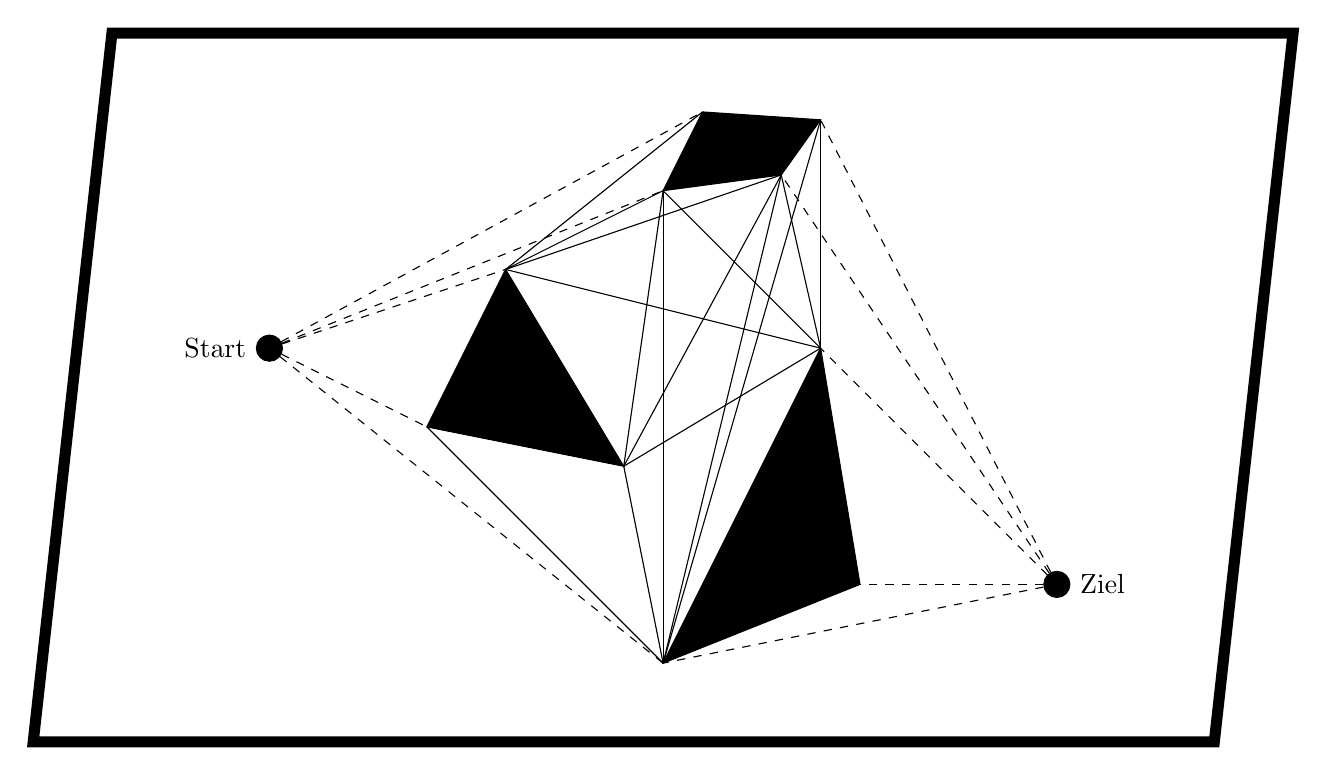
\begin{tikzpicture}
						\node [fill = black, draw, circle, label = left:Start] (S) at (-1, 0) {};
						\node [fill = black, draw, circle, label = right:Ziel] (G) at (9, -3) {};

						\coordinate (a1) at (1, -1);
						\coordinate (a2) at (2, 1);
						\coordinate (a3) at (3.5, -1.5);

						\coordinate (b1) at (4, -4);
						\coordinate (b2) at (6, 0);
						\coordinate (b3) at (6.5, -3);

						\coordinate (c1) at (4, 2);
						\coordinate (c2) at (4.5, 3);
						\coordinate (c3) at (6, 2.9);
						\coordinate (c4) at (5.5, 2.2);

						\coordinate (d1) at (-3, 4);
						\coordinate (d2) at (12, 4);
						\coordinate (d3) at (11, -5);
						\coordinate (d4) at (-4, -5);

						\draw [fill = black] (a1) -- (a2) -- (a3) -- cycle;
						\draw [fill = black] (b1) -- (b2) -- (b3) -- cycle;
						\draw [fill = black] (c1) -- (c2) -- (c3) -- (c4) -- cycle;

						\draw [line width = 4pt] (d1) -- (d2) -- (d3) -- (d4) -- cycle;

						\draw (a1) -- (b1);
						\draw (a2) -- (b2);
						\draw (a2) -- (c1);
						\draw (a2) -- (c2);
						\draw (a2) -- (c4);
						\draw (a3) -- (b1);
						\draw (a3) -- (b2);
						\draw (a3) -- (c1);
						\draw (a3) -- (c4);

						\draw (b1) -- (c1);
						\draw (b1) -- (c3);
						\draw (b1) -- (c4);
						\draw (b2) -- (c1);
						\draw (b2) -- (c3);
						\draw (b2) -- (c4);

						\draw [dashed] (S) -- (a1);
						\draw [dashed] (S) -- (a2);
						\draw [dashed] (S) -- (b1);
						\draw [dashed] (S) -- (c1);
						\draw [dashed] (S) -- (c2);

						\draw [dashed] (G) -- (b1);
						\draw [dashed] (G) -- (b2);
						\draw [dashed] (G) -- (b3);
						\draw [dashed] (G) -- (c3);
						\draw [dashed] (G) -- (c4);
					\end{tikzpicture}
					\caption{Sichtbarkeitsgraph mit Start- und Zielknoten im beschränkten Konfigurationsraum, wobei die schwarzen Flächen Hindernisse darstellen. Zur Vereinfachung wurden die Verbindungen zum Konfigurationsraumrand weggelassen.}
					\label{fig:visibilitygraph}
				\end{figure}
			% end

			\subsubsection{Tangentengraph}
				Der Sichtbarkeitsgraph enthält sehr viel mehr Informationen, als nötig sind (für je zwei Hindernisse sind nur die kotangenten Verbindungen zwischen vier Eckpunkten relevant). Bei einem \emph{Tangentengraph} werden nur diese Verbindungen betrachtet, \dh der Sichtbarkeitsgraph wird auf diese reduziert.
			% end

			\subsubsection{Voronoi-Diagramme}
				Eine Schwierigkeit bei Sichtbarkeitsgraphen ist, dass resultierende Bahnen meistens nahe an Hindernissen vorbei gehen, diese sogar berühren können. Daher sind die durch Sichtbarkeitsgraphen generierten Bahnen nur "semi-frei". Einen alternativen Ansatz verfolgen \emph{Voronoi-Diagramme}, bei denen die Bahnen so weit wie möglich von den nächsten Hindernissen entfernt liegen. Diese werden konstruiert, indem die Wege entlang der Punkte gelegt werden, die den gleichen Abstand zu den nächsten Hindernissen haben (wobei der Rand des Arbeitsbereichs als Hindernis zählt). Dadurch haben die Bahnen immer den maximalen Abstand zu den festen Hindernissen.

				\textbf{Bahnplanung:} Für die Bahnplanung bewegt sich der Roboter zunächst orthogonal zum Voronoi-Diagramm auf dieses zu und bewegt sich anschließend entlang dem Diagramm zum "Absprungpunkt" zum Ziel. Dieser liegt so, dass der Roboter wieder orthogonal zum Diagramm auf das Ziel zubewegt.

				\textbf{Nachteile:}
				\begin{itemize}
					\item Die berechneten Bahnen sind im Vergleich zum Sichtbarkeitsgraphen sehr lang.
					\item Eckige Bahnen, die nur mit Korrekturen in einer kontinuierlichen Bewegung umsetzbar sind.
				\end{itemize}
			% end
		% end

		\subsection{Exakte Zellzerlegung}
			\textbf{Ansatz:} Zerlegung des freien Konfigurationsraums in eine Menge an nicht überlappenden, konvexen Gebieten (Zellen), deren Vereinigung genau den freien Konfigurationsraum ergibt. Über die benachbarten Zellen wird dann der Verbindungsgraph (Freiraumgraph) konstruiert. Abbildung~\ref{fig:connectiongraph} zeigt eine solche Zellzerlegung. \\
			\textbf{Bahnplanung:} Zur Bahnplanung wird ein \emph{Kanal} von der Zelle mit Start zur Zelle mit Ziel konstruiert. Aus diesem Kanal wird anschließend eine Bahn konstruiert, \bspw durch Verbinden der Mittelpunkte der Ränder von benachbarten Zellen.

			\begin{figure}
				\centering
				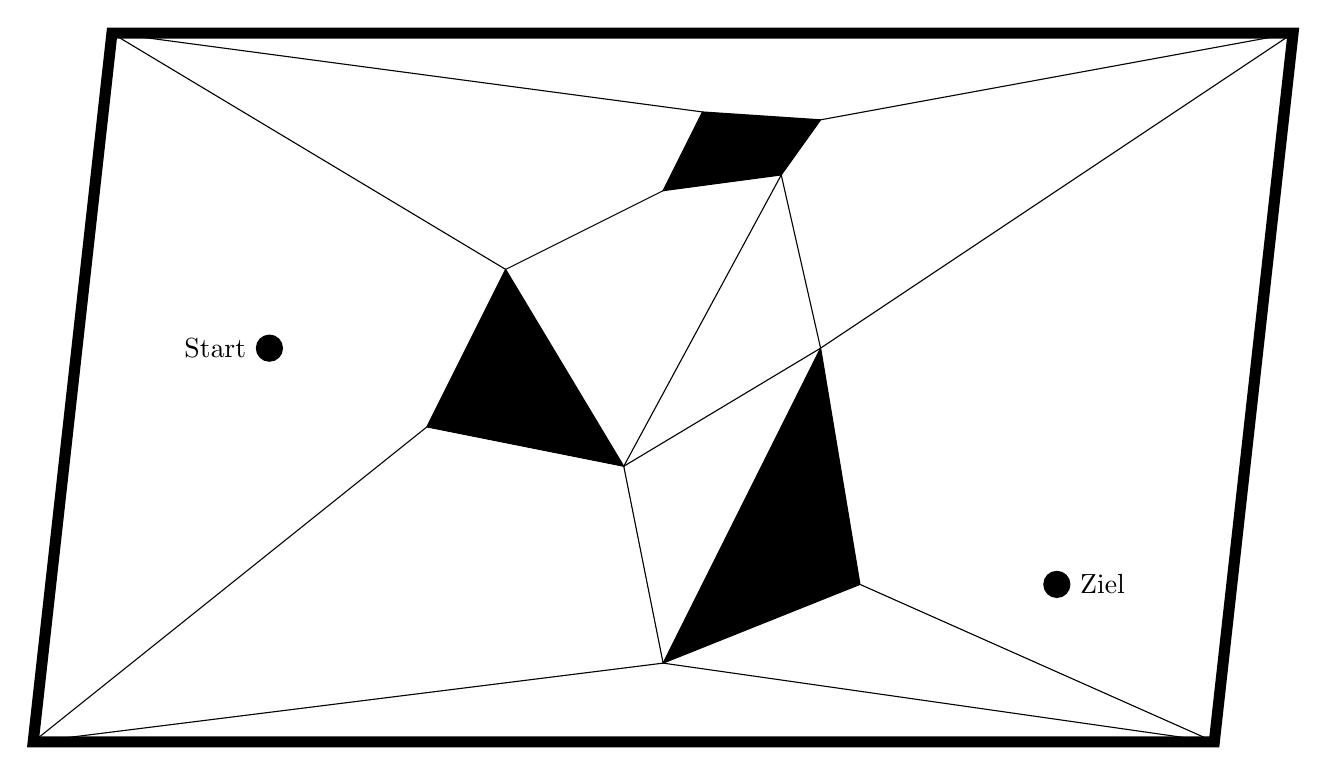
\begin{tikzpicture}
					\node [fill = black, draw, circle, label = left:Start] (S) at (-1, 0) {};
					\node [fill = black, draw, circle, label = right:Ziel] (G) at (9, -3) {};

					\coordinate (a1) at (1, -1);
					\coordinate (a2) at (2, 1);
					\coordinate (a3) at (3.5, -1.5);

					\coordinate (b1) at (4, -4);
					\coordinate (b2) at (6, 0);
					\coordinate (b3) at (6.5, -3);

					\coordinate (c1) at (4, 2);
					\coordinate (c2) at (4.5, 3);
					\coordinate (c3) at (6, 2.9);
					\coordinate (c4) at (5.5, 2.2);

					\coordinate (d1) at (-3, 4);
					\coordinate (d2) at (12, 4);
					\coordinate (d3) at (11, -5);
					\coordinate (d4) at (-4, -5);

					\draw [fill = black] (a1) -- (a2) -- (a3) -- cycle;
					\draw [fill = black] (b1) -- (b2) -- (b3) -- cycle;
					\draw [fill = black] (c1) -- (c2) -- (c3) -- (c4) -- cycle;

					\draw [line width = 4pt] (d1) -- (d2) -- (d3) -- (d4) -- cycle;

					\draw (a1) -- (d4);
					\draw (a2) -- (d1);
					\draw (a2) -- (c1);
					\draw (a3) -- (b1);
					\draw (a3) -- (b2);
					\draw (a3) -- (c4);

					\draw (b1) -- (d3);
					\draw (b1) -- (d4);
					\draw (b2) -- (c4);
					\draw (b2) -- (d2);
					\draw (b3) -- (d3);

					\draw (c2) -- (d1);
					\draw (c3) -- (d2);
				\end{tikzpicture}
				\caption{Zellzerlegung mit Start- und Zielknoten im beschränkten Konfigurationsraum, wobei die schwarzen Flächen Hindernisse darstellen.}
				\label{fig:connectiongraph}
			\end{figure}

			\subsubsection{Trapez-Zerlegung}
				Der Aufwand einer solchen konvexen, optimalen Zellzerlegung ist mindestens polynomial in der Anzahl der Polygonecken der Zerlegung. Eine einfachere Variante stellt die \emph{Trapez-Zerlegung} dar.

				Dabei wird eine vertikale Linie (\bzw Hyper-Ebene) von links nach rechts durch den Konfigurationsraum geschoben. Schneidet sich die Linie mit einem Eckpunkt, so wird eine Gerade vom Schnittpunkt zum Rand, \bzw bis zum nächsten Hindernis erzeugt. Dies führt zu einer Zerlegung in trapezförmige oder dreieckige Zellen.

				Die Bahnplanung funktioniert dann wie bei einer optimalen Zellzerlegung.

				\begin{figure}
					\centering
					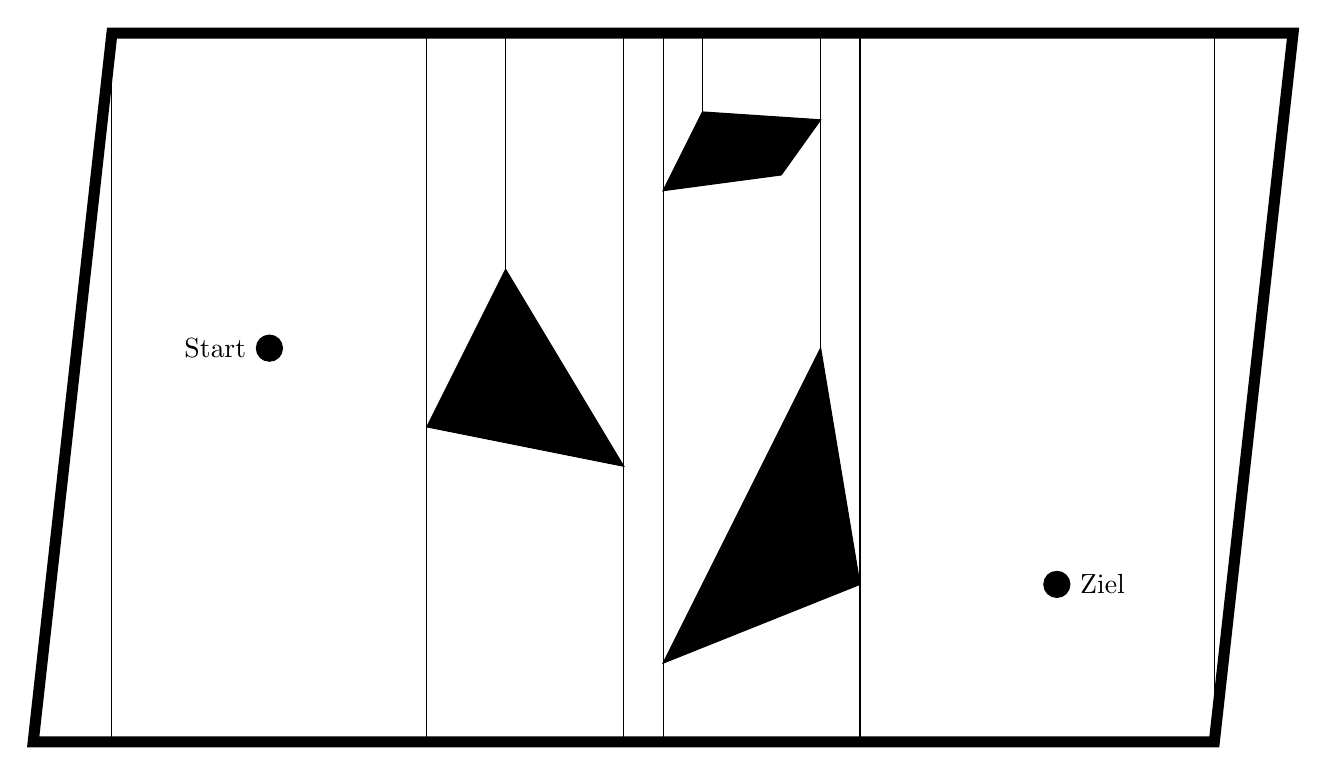
\begin{tikzpicture}
						\node [fill = black, draw, circle, label = left:Start] (S) at (-1, 0) {};
						\node [fill = black, draw, circle, label = right:Ziel] (G) at (9, -3) {};

						\coordinate (a1) at (1, -1);
						\coordinate (a2) at (2, 1);
						\coordinate (a3) at (3.5, -1.5);

						\coordinate (b1) at (4, -4);
						\coordinate (b2) at (6, 0);
						\coordinate (b3) at (6.5, -3);

						\coordinate (c1) at (4, 2);
						\coordinate (c2) at (4.5, 3);
						\coordinate (c3) at (6, 2.9);
						\coordinate (c4) at (5.5, 2.2);

						\coordinate (d1) at (-3, 4);
						\coordinate (d2) at (12, 4);
						\coordinate (d3) at (11, -5);
						\coordinate (d4) at (-4, -5);

						\draw [fill = black] (a1) -- (a2) -- (a3) -- cycle;
						\draw [fill = black] (b1) -- (b2) -- (b3) -- cycle;
						\draw [fill = black] (c1) -- (c2) -- (c3) -- (c4) -- cycle;

						\draw [line width = 4pt] (d1) -- (d2) -- (d3) -- (d4) -- cycle;

						\draw (-3, 4) -- (-3, -5);
						\draw (1, 4) -- (1, -5);
						\draw (2, 4) -- (2, 1);
						\draw (3.5, 4) -- (3.5, -5);
						\draw (4, 4) -- (4, -5);
						\draw (4.5, 4) -- (4.5, 3);
						\draw (6, 4) -- (6, 0);
						\draw (6.5, 4) -- (6.5, -5);
						\draw (11, 4) -- (11, -5);
					\end{tikzpicture}
					\caption{Trapez-Zerlegung mit Start- und Zielknoten im beschränkten Konfigurationsraum, wobei die schwarzen Flächen Hindernisse darstellen.}
					\label{fig:connectiongraphtrapeze}
				\end{figure}
			% end
		% end

		\subsection{Approximative Zellzerlegung}
			Ein Vorteil der Zellzerlegung liegt darin, dass lokale Änderungen der Umwelt nur lokale Änderungen der Repräsentation (im Unterschied zum Roadmap-Verfahren). Bei der exakten Zellzerlegung ergibt die Vereinigung der Zellen exakt den Freiraum. Eine approximative Zellzerlegung
			\begin{itemize}
				\item verwendet nur Zellen fester, vorgegebener Größe(n),
				\item die Vereinigung der Zellen ist eine Teilmenge des Freiraums und
				\item der Rand einer Zelle hat meistens keine physikalische Bedeutung.
			\end{itemize}
			Wie in Abbildung~\ref{fig:approxcelldecomposition} wird der Raum rekursiv in immer vier gleich Große Zellen zerlegt. Daraus kann ein Quadtree erstellt werden, dessen Knoten die folgenden Werte haben können:
			\begin{itemize}
				\item Nur Freiraum:  \tabto{3cm} \whiteBox
				\item Nur Hindernis: \tabto{3cm} \blackBox
				\item Gemischt:      \tabto{3cm} \grayBox
			\end{itemize}
			Der Raum wird solange weiter zerlegt, bis die maximale Auflösung erreicht wurde. Die Knoten werden dabei in der Reihenfolge
			\begin{table}[H]
				\centering
				\begin{tabular}{|c|c|}
					\hline
					\num{1} & \num{2} \\ \hline
					\num{3} & \num{4} \\ \hline
				\end{tabular}
			\end{table}
			von links nach rechts gelistet. Abbildung~\ref{fig:approxcelldecompositionquadtree} zeigt den Quadtree des vierten Quadranten der approximativen Zerlegung aus Abbildung~\ref{fig:approxcelldecomposition}.

			Das Verfahren lässt sich analog auf einen 3- oder \(n\)-dimensionalen Raum anwenden.

			\begin{figure}
				\centering
				\begin{tikzpicture}
					\coordinate (a1) at (1, -1);
					\coordinate (a2) at (2, 1);
					\coordinate (a3) at (3.5, -1.5);

					\coordinate (b1) at (4, -4);
					\coordinate (b15) at (5, 0);
					\coordinate (b2) at (6.5, 1);
					\coordinate (b3) at (6.5, -3);

					\coordinate (c1) at (4, 2);
					\coordinate (c2) at (4.5, 3);
					\coordinate (c3) at (6, 2.9);
					\coordinate (c4) at (5.5, 2.2);

					\coordinate (d1) at (-1, 5);
					\coordinate (d2) at (9, 5);
					\coordinate (d3) at (9, -5);
					\coordinate (d4) at (-1, -5);

					\draw [fill = black] (a1) -- (a2) -- (a3) -- cycle;
					\draw [fill = black] (b1) -- (b15) -- (b2) -- (b3) -- cycle;
					\draw [fill = black] (c1) -- (c2) -- (c3) -- (c4) -- cycle;

					\draw [line width = 4pt] (d1) -- (d2) -- (d3) -- (d4) -- cycle;

					\draw [color = TUDa-3b, line width = 3pt, step = 5, xshift = -1cm] (d1) grid +(10, -10);
					\draw [color = TUDa-3b, line width = 2pt, step = 2.5, xshift = -1cm] (d1) grid +(10, -10);
					\draw [color = TUDa-3b, line width = 1pt] (0.25, 0) -- (0.25, -2.5);
					\draw [color = TUDa-3b, line width = 1pt] (2.75, 2.5) -- (2.75, -2.5);
					\draw [color = TUDa-3b, line width = 1pt] (5.25, 5) -- (5.25, -5);
					\draw [color = TUDa-3b, line width = 1pt] (-1, -1.25) -- (6.5, -1.25);
					\draw [color = TUDa-3b, line width = 1pt] (4, -3.75) -- (6.5, -3.75);
					\draw [color = TUDa-3b, line width = 1pt] (1.5, 1.25) -- (6.5, 1.25);
					\draw [color = TUDa-3b, line width = 1pt] (4, 3.75) -- (6.5, 3.75);
				\end{tikzpicture}
				\caption{Approximative Zellzerlegung im beschränkten Konfigurationsraum, wobei die schwarzen Flächen Hindernisse darstellen.}
				\label{fig:approxcelldecomposition}
			\end{figure}

			\begin{figure}
				\Tree[.{\grayBox}
					[.{\grayBox}
						{\grayBox}
						{\blackBox}
						{\grayBox}
						{\blackBox}
					]
					{\whiteBox}
					[.{\grayBox}
						{\grayBox}
						{\grayBox}
						{\grayBox}
						{\whiteBox}
					]
					{\whiteBox}
				]
				\caption{Quadtree des vierten Quadranten der approximativen Zerlegung aus Abbildung~\ref{fig:approxcelldecomposition}.}
				\label{fig:approxcelldecompositionquadtree}
			\end{figure}
		% end

		\subsection{Potentialfeld-Methoden} % 7.50, 7.51, 7.52, 7.53, 7.54, 7.55, 7.56
			Zerlegungs-Verfahren beruhen auf der Suche in einem diskreten (\bzw diskretisierten) Raum. Eine alternative sind Heuristiken zur (lokalen) Suche in einem kontinuierlichem Raum.

			Bei \emph{Potentialfeld-Methoden} werden Objekte als geladene, punktförmige Teilchen betrachtet, wobei das
			\begin{itemize}
				\item Ziel \( \vec{q}_\text{Ziel} \) ein anziehendes Potential \( U_\text{Ziel} \) hat und
				\item Hindernisse ein abstoßendes Potential \( U_\text{Hindernis} \) haben.
			\end{itemize}
			Daraus ergibt für jede Konfiguration \( \vec{q} \) ein Potential \(U\):
			\begin{equation*}
				U(\vec{q}) = U_\text{Ziel}(\vec{q}) + \sum U_\text{Hindernis}(\vec{q})
			\end{equation*}
			Auf den Roboter wirkt dann eine fiktive Anziehungskraft als Gradient des Potentialfelds:
			\begin{equation*}
				\vec{F}(\vec{q}) = -\vec{\nabla} U(\vec{q}) =
				- \begin{bmatrix}
					\partial U / \partial q_1 \\
					\vdots                    \\
					\partial U / \partial q_n
				\end{bmatrix}
			\end{equation*}
			Dies entspricht dem Verfahren des steilsten Abstiegs (Steepest Descent) zur Minimierung des Gesamtpotentials.

			\paragraph{Berechnung}
				Es sind viele verschiedene Definitionen der Potentiale möglich, z.\,B.:
				\begin{align*}
					U_\text{Ziel}(\vec{q})      & \coloneqq \alpha \cdot \text{dist}(\vec{q}, \text{Ziel})^2               \\
					U_\text{Hindernis}(\vec{q}) & \coloneqq \frac{\beta}{\beta_0 + \text{dist}(\vec{q}, \text{Hindernis})}
				\end{align*}
				mit geeigneten zu wählenden Parametern \( \alpha, \beta, \beta_0 > 0 \), wobei \( \beta_0 \) die Potentialhöhe der Hindernisse festlegt (\( \beta_0 = 0 \) entspricht einem unendlichen Potential, \dh einer Barriere). \( \text{dist}(\vec{q}, \text{Hindernis}) \) entspricht dem minimalen Abstand des Punktes zum Hindernis, wobei "Null" bedeutet, dass der Punkt im Hindernis liegt.

				Für \( U_\text{Hindernis}(\vec{q}) \) gibt es unterschiedliche Berechnungsvarianten, z.\,B.:
				\begin{itemize}
					\item nur zum nächsten Hindernis oder
					\item summiert über alle Hindernisse (in der Nähe).
				\end{itemize}
			% end

			\paragraph{Diskussion}
				\begin{itemize}
					\item \textbf{Vorteile:}
						\begin{itemize}
							\item Einfache Algorithmen.
							\item Glatte Bahnformen.
							\item Online einsetzbar, \dh die Planung mit aktuellen Sensordaten ist in Echtzeit mit der Regelung koppelbar.
						\end{itemize}
					\item \textbf{Nachteil:}
						\begin{itemize}
							\item Die Gefahr, in lokalen Minima hängen zu bleiben, ist groß.
						\end{itemize}
				\end{itemize}

				Abhilfen \bzgl der lokalen Minima sind z.\,B.:
				\begin{itemize}
					\item Konstruktion eines Potentials ohne lokales Minima, \zB über Strömungsmodelle (hohe Rechenzeiten).
					\item Erhöhung des Abstoßungspotentials in einer Region, in der ein lokales Minima erkannt wurde (dieses als Hindernis markieren).
					\item Kopplung der lokalen Potentialfeld-Methode mit einem globalen Verfahren:
						\begin{itemize}
							\item Randomisierte Bahnplaner (entkommen aus den Minima durch stochastische Suche).
							\item Verwendung von globalen Zellzerlegungs-Verfahren zur Generierung einer Ausgangsbahn.
						\end{itemize}
				\end{itemize}
			% end
		% end

		\subsection{Komplexität der geometrischen Bahnplanung}
			Eine obere Schranke der Komplexität der (globalen) Bahnplanung im Konfigurationsraum wurde von Schwartz und Sharir im Jahre 1983 gefunden:
			\begin{itemize}
				\item Die Komplexität des Problems wächst (vermutlich immer) exponentiell in der Anzahl der Roboterfreiheitsgrade.
				\item Wenn es schnellere Algorithmen geben sollte, so benötigen diese mindestens polynomiale Zeit \bzgl \(n\).
			\end{itemize}

			Anmerkungen:
			\begin{itemize}
				\item In Spezialfällen mit besonderen Geometrien kann die Komplexität niedriger sein.
				\item Im Allgemeinen wächst die Komplexität weiter an, wenn sich die Hindernisse bewegen und/oder Unsicherheiten berücksichtigt werden.
				\item Alle gängigen Bahnplanungsverfahren sind "unvollständig" \bzw beruhen auf Heuristiken oder Diskretisierungen.
			\end{itemize}
		% end

		\subsection{Stichprobenverfahren}
			Ein Stichprobenverfahren zur Erstellung einer \emph{Probabilistic Roadmap} (PRM) besteht aus folgenden Schritten:
			\begin{enumerate}
				\item Generieren von zufälligen Stichproben von Konfigurationen (Abbildung~\ref{fig:prmstep1}).
				\item Entfernen von Stichproben im verbotenem Bereich (Abbildung~\ref{fig:prmstep2}).
				\item Verbinden jeder Stichproben mit den \(k\) nächsten (noch nicht verbundenen) Nachbarn (Abbildung~\ref{fig:prmstep3}).
				\item Entfernen von allen Verbindungen, die durch eine verbotene Region gehen (Abbildung~\ref{fig:prmstep4}).
			\end{enumerate}
			Der daraus entstehende (\mglw nicht-planare) Graph ist eine "probabilistische Straßenkarte" (Probabilistic Roadmap, PRM) (Abbildung~\ref{fig:prmstep5}). Die Bahnplanung kann dann unter Verwendung von Graphenalgorithmen (\zB A*) stattfinden.

			\begin{figure}
				\centering
				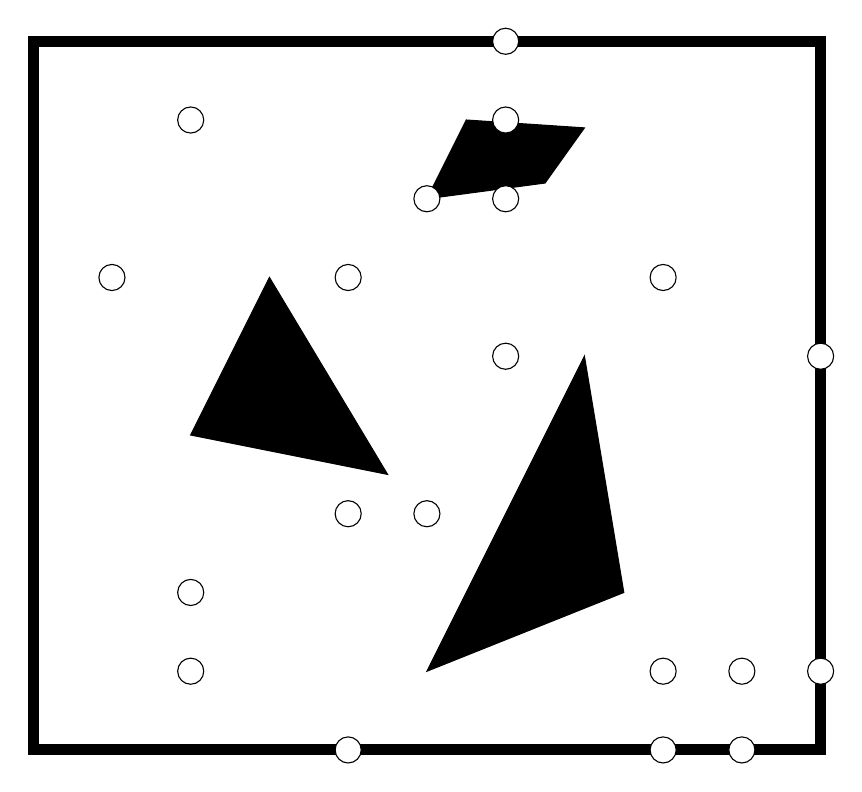
\begin{tikzpicture}
					\coordinate (a1) at (1, -1);
					\coordinate (a2) at (2, 1);
					\coordinate (a3) at (3.5, -1.5);

					\coordinate (b1) at (4, -4);
					\coordinate (b2) at (6, 0);
					\coordinate (b3) at (6.5, -3);

					\coordinate (c1) at (4, 2);
					\coordinate (c2) at (4.5, 3);
					\coordinate (c3) at (6, 2.9);
					\coordinate (c4) at (5.5, 2.2);

					\coordinate (d1) at (-1, 4);
					\coordinate (d2) at (9, 4);
					\coordinate (d3) at (9, -5);
					\coordinate (d4) at (-1, -5);

					\draw [fill = black] (a1) -- (a2) -- (a3) -- cycle;
					\draw [fill = black] (b1) -- (b2) -- (b3) -- cycle;
					\draw [fill = black] (c1) -- (c2) -- (c3) -- (c4) -- cycle;

					\draw [line width = 4pt] (d1) -- (d2) -- (d3) -- (d4) -- cycle;

					\node [draw, circle, fill = white] (a) at (0, 1) {};
					\node [draw, circle, fill = white] (b) at (4, 2) {};
					\node [draw, circle, fill = white] (c) at (7, -4) {};
					\node [draw, circle, fill = white] (d) at (5, 2) {};
					\node [draw, circle, fill = white] (e) at (3, 1) {};
					\node [draw, circle, fill = white] (f) at (3, -2) {};
					\node [draw, circle, fill = white] (g) at (7, -5) {};
					\node [draw, circle, fill = white] (h) at (4, -2) {};
					\node [draw, circle, fill = white] (i) at (8, -5) {};
					\node [draw, circle, fill = white] (j) at (9, -4) {};
					\node [draw, circle, fill = white] (k) at (1, -4) {};
					\node [draw, circle, fill = white] (l) at (9, 0) {};
					\node [draw, circle, fill = white] (m) at (5, 0) {};
					\node [draw, circle, fill = white] (n) at (8, -4) {};
					\node [draw, circle, fill = white] (o) at (5, 4) {};
					\node [draw, circle, fill = white] (p) at (7, 1) {};
					\node [draw, circle, fill = white] (q) at (1, 3) {};
					\node [draw, circle, fill = white] (r) at (1, -3) {};
					\node [draw, circle, fill = white] (s) at (5, 3) {};
					\node [draw, circle, fill = white] (t) at (3, -5) {};
				\end{tikzpicture}
				\caption{Probabilistic Roadmap, Schritt 1: Zufällige Stichproben von Konfigurationen.}
				\label{fig:prmstep1}
			\end{figure}
			\begin{figure}
				\centering
				\begin{tikzpicture}
					\coordinate (a1) at (1, -1);
					\coordinate (a2) at (2, 1);
					\coordinate (a3) at (3.5, -1.5);

					\coordinate (b1) at (4, -4);
					\coordinate (b2) at (6, 0);
					\coordinate (b3) at (6.5, -3);

					\coordinate (c1) at (4, 2);
					\coordinate (c2) at (4.5, 3);
					\coordinate (c3) at (6, 2.9);
					\coordinate (c4) at (5.5, 2.2);

					\coordinate (d1) at (-1, 4);
					\coordinate (d2) at (9, 4);
					\coordinate (d3) at (9, -5);
					\coordinate (d4) at (-1, -5);

					\draw [fill = black] (a1) -- (a2) -- (a3) -- cycle;
					\draw [fill = black] (b1) -- (b2) -- (b3) -- cycle;
					\draw [fill = black] (c1) -- (c2) -- (c3) -- (c4) -- cycle;

					\draw [line width = 4pt] (d1) -- (d2) -- (d3) -- (d4) -- cycle;

					\node [draw, circle, fill = white] (a) at (0, 1) {};
					\node [draw, circle, fill = white] (c) at (7, -4) {};
					\node [draw, circle, fill = white] (e) at (3, 1) {};
					\node [draw, circle, fill = white] (f) at (3, -2) {};
					\node [draw, circle, fill = white] (h) at (4, -2) {};
					\node [draw, circle, fill = white] (k) at (1, -4) {};
					\node [draw, circle, fill = white] (m) at (5, 0) {};
					\node [draw, circle, fill = white] (n) at (8, -4) {};
					\node [draw, circle, fill = white] (p) at (7, 1) {};
					\node [draw, circle, fill = white] (q) at (1, 3) {};
					\node [draw, circle, fill = white] (r) at (1, -3) {};
					\node [draw, circle, fill = TUDa-9b] (b) at (4, 2) {};
					\node [draw, circle, fill = TUDa-9b] (d) at (5, 2) {};
					\node [draw, circle, fill = TUDa-9b] (g) at (7, -5) {};
					\node [draw, circle, fill = TUDa-9b] (i) at (8, -5) {};
					\node [draw, circle, fill = TUDa-9b] (j) at (9, -4) {};
					\node [draw, circle, fill = TUDa-9b] (l) at (9, 0) {};
					\node [draw, circle, fill = TUDa-9b] (o) at (5, 4) {};
					\node [draw, circle, fill = TUDa-9b] (s) at (5, 3) {};
					\node [draw, circle, fill = TUDa-9b] (t) at (3, -5) {};
				\end{tikzpicture}
				\caption{Probabilistic Roadmap, Schritt 2: Entfernung der "verbotenen" Stichproben.}
				\label{fig:prmstep2}
			\end{figure}
			\begin{figure}
				\centering
				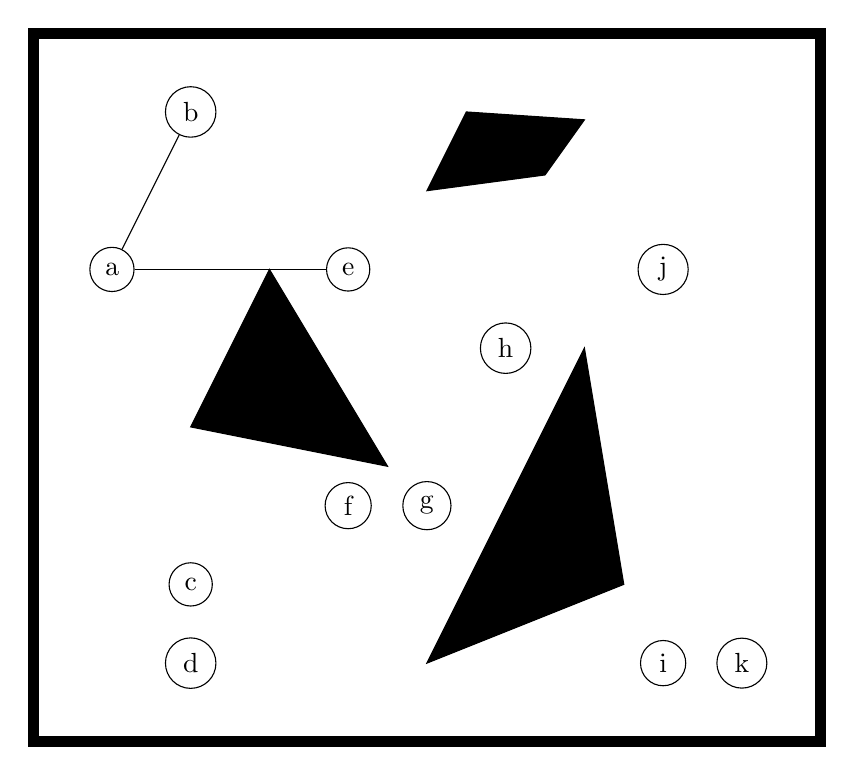
\begin{tikzpicture}
					\coordinate (a1) at (1, -1);
					\coordinate (a2) at (2, 1);
					\coordinate (a3) at (3.5, -1.5);

					\coordinate (b1) at (4, -4);
					\coordinate (b2) at (6, 0);
					\coordinate (b3) at (6.5, -3);

					\coordinate (c1) at (4, 2);
					\coordinate (c2) at (4.5, 3);
					\coordinate (c3) at (6, 2.9);
					\coordinate (c4) at (5.5, 2.2);

					\coordinate (d1) at (-1, 4);
					\coordinate (d2) at (9, 4);
					\coordinate (d3) at (9, -5);
					\coordinate (d4) at (-1, -5);

					\draw [fill = black] (a1) -- (a2) -- (a3) -- cycle;
					\draw [fill = black] (b1) -- (b2) -- (b3) -- cycle;
					\draw [fill = black] (c1) -- (c2) -- (c3) -- (c4) -- cycle;

					\draw [line width = 4pt] (d1) -- (d2) -- (d3) -- (d4) -- cycle;

					\node [draw, circle, fill = white] (a) at (0, 1) {a};
					\node [draw, circle, fill = white] (b) at (1, 3) {b};
					\node [draw, circle, fill = white] (c) at (1, -3) {c};
					\node [draw, circle, fill = white] (d) at (1, -4) {d};
					\node [draw, circle, fill = white] (e) at (3, 1) {e};
					\node [draw, circle, fill = white] (f) at (3, -2) {f};
					\node [draw, circle, fill = white] (g) at (4, -2) {g};
					\node [draw, circle, fill = white] (h) at (5, 0) {h};
					\node [draw, circle, fill = white] (i) at (7, -4) {i};
					\node [draw, circle, fill = white] (j) at (7, 1) {j};
					\node [draw, circle, fill = white] (k) at (8, -4) {k};

					\draw (a) -- (b);
					\draw (a) -- (e);
				\end{tikzpicture}
				\caption{Probabilistic Roadmap, Schritt 3: Verbinden jeder gültigen Stichprobe mit den \( k = 2 \) nächsten Nachbar.}
				\label{fig:prmstep3}
			\end{figure}
			\begin{figure}
				\centering
				\begin{tikzpicture}
					\coordinate (a1) at (1, -1);
					\coordinate (a2) at (2, 1);
					\coordinate (a3) at (3.5, -1.5);

					\coordinate (b1) at (4, -4);
					\coordinate (b2) at (6, 0);
					\coordinate (b3) at (6.5, -3);

					\coordinate (c1) at (4, 2);
					\coordinate (c2) at (4.5, 3);
					\coordinate (c3) at (6, 2.9);
					\coordinate (c4) at (5.5, 2.2);

					\coordinate (d1) at (-1, 4);
					\coordinate (d2) at (9, 4);
					\coordinate (d3) at (9, -5);
					\coordinate (d4) at (-1, -5);

					\draw [fill = black] (a1) -- (a2) -- (a3) -- cycle;
					\draw [fill = black] (b1) -- (b2) -- (b3) -- cycle;
					\draw [fill = black] (c1) -- (c2) -- (c3) -- (c4) -- cycle;

					\draw [line width = 4pt] (d1) -- (d2) -- (d3) -- (d4) -- cycle;

					\node [draw, circle, fill = white] (a) at (0, 1) {a};
					\node [draw, circle, fill = white] (b) at (1, 3) {b};
					\node [draw, circle, fill = white] (c) at (1, -3) {c};
					\node [draw, circle, fill = white] (d) at (1, -4) {d};
					\node [draw, circle, fill = white] (e) at (3, 1) {e};
					\node [draw, circle, fill = white] (f) at (3, -2) {f};
					\node [draw, circle, fill = white] (g) at (4, -2) {g};
					\node [draw, circle, fill = white] (h) at (5, 0) {h};
					\node [draw, circle, fill = white] (i) at (7, -4) {i};
					\node [draw, circle, fill = white] (j) at (7, 1) {j};
					\node [draw, circle, fill = white] (k) at (8, -4) {k};

					\draw (a) -- (b);
					\draw [color = TUDa-9b] (a) -- (e);

					\draw (b) -- (e);
					\draw (b) -- (h);

					\draw (c) -- (d);
					\draw (c) -- (f);

					\draw (d) -- (f);
					\draw (d) -- (g);

					\draw (e) -- (h);
					\draw [color = TUDa-9b] (e) -- (f);

					\draw (f) -- (g);
					\draw [color = TUDa-9b] (f) -- (h);

					\draw [color = TUDa-9b] (g) -- (i);
					\draw [color = TUDa-9b] (g) -- (j);

					\draw (h) -- (g);
					\draw (h) -- (j);

					\draw (i) -- (k);
					\draw (i) -- (j);

					\draw (j) -- (e);
					\draw (j) -- (f);

					\draw [color = TUDa-9b] (k) -- (g);
					\draw [color = TUDa-9b] (k) -- (h);
				\end{tikzpicture}
				\caption{Probabilistic Roadmap, Schritt 4: Entfernen der "verbotenen" Verbindungen.}
				\label{fig:prmstep4}
			\end{figure}
			\begin{figure}
				\centering
				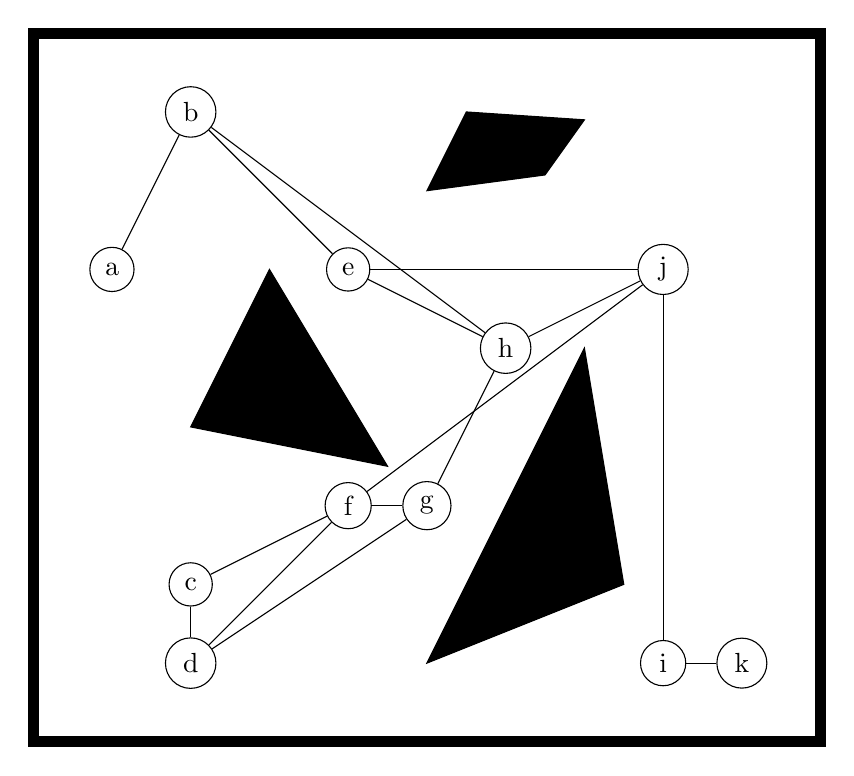
\begin{tikzpicture}
					\coordinate (a1) at (1, -1);
					\coordinate (a2) at (2, 1);
					\coordinate (a3) at (3.5, -1.5);

					\coordinate (b1) at (4, -4);
					\coordinate (b2) at (6, 0);
					\coordinate (b3) at (6.5, -3);

					\coordinate (c1) at (4, 2);
					\coordinate (c2) at (4.5, 3);
					\coordinate (c3) at (6, 2.9);
					\coordinate (c4) at (5.5, 2.2);

					\coordinate (d1) at (-1, 4);
					\coordinate (d2) at (9, 4);
					\coordinate (d3) at (9, -5);
					\coordinate (d4) at (-1, -5);

					\draw [fill = black] (a1) -- (a2) -- (a3) -- cycle;
					\draw [fill = black] (b1) -- (b2) -- (b3) -- cycle;
					\draw [fill = black] (c1) -- (c2) -- (c3) -- (c4) -- cycle;

					\draw [line width = 4pt] (d1) -- (d2) -- (d3) -- (d4) -- cycle;

					\node [draw, circle, fill = white] (a) at (0, 1) {a};
					\node [draw, circle, fill = white] (b) at (1, 3) {b};
					\node [draw, circle, fill = white] (c) at (1, -3) {c};
					\node [draw, circle, fill = white] (d) at (1, -4) {d};
					\node [draw, circle, fill = white] (e) at (3, 1) {e};
					\node [draw, circle, fill = white] (f) at (3, -2) {f};
					\node [draw, circle, fill = white] (g) at (4, -2) {g};
					\node [draw, circle, fill = white] (h) at (5, 0) {h};
					\node [draw, circle, fill = white] (i) at (7, -4) {i};
					\node [draw, circle, fill = white] (j) at (7, 1) {j};
					\node [draw, circle, fill = white] (k) at (8, -4) {k};

					\draw (a) -- (b);

					\draw (b) -- (e);
					\draw (b) -- (h);

					\draw (c) -- (d);
					\draw (c) -- (f);

					\draw (d) -- (f);
					\draw (d) -- (g);

					\draw (e) -- (h);

					\draw (f) -- (g);

					\draw (h) -- (g);
					\draw (h) -- (j);

					\draw (i) -- (k);
					\draw (i) -- (j);

					\draw (j) -- (e);
					\draw (j) -- (f);
				\end{tikzpicture}
				\caption{Probabilistic Roadmap, Ergebnis: Der resultierende (nicht-planare) Graph ist die Probabilistic Roadmap (PRM)}
				\label{fig:prmstep5}
			\end{figure}

			\paragraph{Allgemeines Vorgehen}
				Das allgemeine Vorgehen von Stichprobenverfahren ist erst die Diskretisierung durch Stichproben und anschließende Graphensuche. Dabei gibt es zwei Kategorien von Graphbasierten Verfahren:
				\begin{itemize}
					\item Informiertes (heuristisches) Suchen
					\item Uninformiertes (blindes) Suchen
				\end{itemize}
				Es ist wichtig, dass die Stichproben "gut" gewählt werden, z.\,B.:
				\begin{itemize}
					\item Gleichförmige Stichprobenverteilung
					\item mehr Stichproben bei Punkten mit wenigen Nachbarn
					\item mehr Stichproben bei Hindernissen
				\end{itemize}

				Durch korrekte (zulässige) Heuristiken kann eine enorme Performanzverbesserung erzielt werden. In der Praxis ist die Auswahl solcher Heuristiken jedoch kompliziert\dots
			% end
		% end

		\subsection{Rapidly Exploring Random Trees (RRTs)}
			Siehe Algorithmus~\ref{alg:rrt}.

			\begin{algorithm}
				\KwData{\( x_\mathit{init} \), \( K \), \( \Delta t \)}
				\Begin{
					\(\mathcal{T}.\text{init}(x_\mathit{init}) \) \;
					\For{\( k = 1 \) to \( K \)}{
						\( x_\mathit{rand} \gets \text{RANDOM\_STATE}() \) \;
						\( x_\mathit{near} \gets \text{NEAREST\_NEIGHBOR}(x_\mathit{rand}, \mathcal{T}) \) \;
						\( u \gets \text{SELECT\_INPUT}(x_\mathit{rand}, x_\mathit{near}) \) \;
						\( x_\mathit{new} \gets \text{NEW\_STATE}(x_\mathit{near}, u, \Delta t) \) \;
						\( \mathcal{T}.\text{add\_vertex}(x_\mathit{new}) \) \;
						\( \mathcal{T}.\text{add\_edge}(x_\mathit{near}, x_\mathit{new}, u) \) \;
					}
					\Return \(\mathcal{T}\) \;
				}
				\caption{Rapidly Exploring Random Trees}
				\label{alg:rrt}
			\end{algorithm}
		% end

		\subsection{Beispiel: MINERVA}
			MINERVA ist ein Museumstourführungsroboter.

			\subsubsection{Umweltmodell: Belegungskarte}
				\begin{itemize}
					\item Die Umgebungskarte wird eingeteilt in ein Netz aus quadratischen Zellen, wobei freie Stellen hell und Hindernisse dunkel markiert werden.
					\item Diese \emph{Belegungskarte} erlernt der Roboter selbstständig (durch Herumfahren).
					\item Die Verknüpfung der beiden Problemstellungen (Aufbau einer Karte und Bestimmung der Position/Orientierung) wird als \emph{SLAM} (Self Localization and Mapping) bezeichnet (siehe Abschnitt~\ref{sec:slam}).
					\item Die Bewegungskarte wird dabei in zwei Schritten aufgebaut:
						\begin{enumerate}
							\item Erfassung von Laser-, Sonar und Odometriedaten.
							\item Fusion der Sensordaten zur Berechnung der Umgebungskarte und der Position/Orientierung des Roboters.
						\end{enumerate}
					\item Die Bahnplanung (mittels Kostenminimierung) erfolgt anschließend auf Basis der Belegungskarte, wobei diese während der Fahrt bei Bedarf neu berechnet wird.
					\item Schwierigkeiten:
						\begin{itemize}
							\item Kürzeste-Wege-Planer sind prinzipiell einsetzbar, allerdings ist in weiten, offenen Umgebung das Versagen der externen Distanzsensoren möglich.
							\item Eine Abhilfe ist, bei der Bahnplanung die für Sensoren günstigen Positionen zu berücksichtigen (\zB nahe am Rand).
						\end{itemize}
				\end{itemize}
			% end

			\subsubsection{"Küstennahe" Bahnplanung}
				Bei der "küstennahen" Bahnplanung wird versucht, den Roboter möglichst nah an Wänden (\bzw Allgemein dem Rand der Karte) zu fahren.
			% end

			\subsubsection{Kollisionsvermeidung (MINERVA)}
				\begin{itemize}
					\item Das Kollisionsvermeidungs-Modul steuert sowohl die momentane Bewegungsrichtung als auch die Geschwindigkeit.
					\item Dabei wird die Roboterkinematik und -dynamik berücksichtigt (Masseträgheiten, maximale und minimale Drehmomente der Radantriebe).
					\item \(\mu\text{DWA}\) (Dynamic Window Algorithm):
						\begin{itemize}
							\item Eingabe: Rohe Abstandsmesswerte (sowohl gemessene als auch simulierte) und Zielposition.
							\item Ausgabe: Sollwert für die lineare und Drehwinkel-Geschwindigkeit.
							\item Berücksichtigung von: harten Beschränkungen (der Roboter muss immer vor dem Aufprall auf ein Hindernis zum Stehen) kommen müssen sowie von weichen Beschränkungen (maximale/minimale Momente, Abstand zum Ziel verringern, Abstand zu Hindernissen groß halten (unterschiedlich Gewichtet)).
						\end{itemize}
				\end{itemize}
			% end
		% end
	% end

	\section{Kinematische und dynamische Trajektorienplanung}
		Bei der kinematischen und dynamischen (kinetischen) Trajektorienplanung werden zusätzlich zu den geometrischen Anforderungen auch die kinematischen \bzw kinetischen Anforderungen des Robotermodells berücksichtigt.

		\subsection{Allgemeine Formulierung}
			Es ist die Systemdynamik
			\begin{equation*}
				\dot{\vec{x}}(t) = \vec{f}\big(\vec{x}(t), \vec{u}(t), t\big) =
				\begin{bmatrix}
					f_1\big(\vec{x}(t), \vec{u}(t), t\big) \\
					\vdots                                 \\
					f_m\big(\vec{x}(t), \vec{u}(t), t\big)
				\end{bmatrix}
			\end{equation*}
			mit den Zustandsvariablen \( \vec{x}(t) = \begin{bmatrix} x_1(t) & \cdots & x_m(t) \end{bmatrix}^T \) und den Steuergrößen \( \vec{u}(t) = \begin{bmatrix} u_1(t) & \cdots & u_l(t) \end{bmatrix}^T \), die bestimmten Steuerbeschränkungen
			\begin{equation*}
				\vec{u}(t) \leq \vec{u}_\mathit{max} \quad\iff\quad
				\begin{matrix}
					u_1(t) \leq u_{1, \mathit{max}} \\
					\vdots                          \\
					u_l(t) \leq u_{l, \mathit{max}}
				\end{matrix}
			\end{equation*}
			unterliegen. Für Anfangswerte \( \vec{x}(0) \) und Endwerte \( \vec{x}(t_f) \) unterliegt das gesamte System im Zeitraum \( 0 \leq t \leq t_f \) außerdem bestimmten Zustandsbeschränkungen:
			\begin{equation*}
				\vec{g}\big(\vec{x}(t), \vec{u}(t), t\big) \geq \vec{0} \quad\iff\quad
				\begin{matrix}
					g_1\big(\vec{x}(t), \vec{u}(t), t\big) \geq 0 \\
					\vdots                                        \\
					g_n\big(\vec{x}(t), \vec{u}(t), t\big) \geq 0
				\end{matrix}
			\end{equation*}

			Das \emph{optimale Steuerungsproblem} (Optimal Control Problem) lässt sich nun durch ein Gütekriterium/eine Kostenfunktion wie folgt definieren
			\begin{equation*}
				\min_{\vec{u}} \> J(\vec{x}, \vec{u}) = \Phi\big(\vec{x}(t_f), t_f\big) + \int_{0}^{t_f} \! L\big(\vec{x}(t), \vec{u}(t), t\big) \dd{t}
			\end{equation*}
			wobei die Kostenfunktion \( J(\vec{x}, \vec{u}) \) in zwei Funktionen \( \Phi \) und \( L \) aufgespalten wird. Beispielhafte Gütekriterien sind:
			\begin{itemize}
				\item Zeitminimalität (\(t_f\) frei):
			\end{itemize}
			\begin{gather*}
				\Phi = t_f,\quad L = 0 \quad\implies\quad \min_{\vec{u}} \> J_t(\vec{x}, \vec{u}) = t_f
			\end{gather*}
			\begin{itemize}
				\item Energieminimalität (\(t_f\) vorgegeben):
			\end{itemize}
			\begin{equation*}
				\Phi = 0,\quad L = \sum_{i = 1}^{l} u_i^2 (t) \quad\implies\quad \min_{\vec{u}} \> J_e(\vec{x}, \vec{u}) = \int_{0}^{t_f} \! \sum_{i = 1}^{l} u_i^2 (t) \dd{t}
			\end{equation*}
			\begin{itemize}
				\item Kombiniertes Kriterium (\(t_f\) frei):
			\end{itemize}
			\begin{equation*}
				\min_{\vec{u}} \> J(\vec{x}, \vec{u}) = \rho_1 \cdot J_t(\vec{x}, \vec{u}) + \rho_2 \cdot J_e(\vec{x}, \vec{u}),\quad \rho_1, \rho_2 > 0
			\end{equation*}

			Siehe auch Vorlesung "Optimierung statischer und dynamischer Systeme".
		% end
	% end
% end

\chapter{Navigation mobiler Roboter}
	\emph{Navigation} ist die Fähigkeit, den Kurs (die Fahrt) eines mobilen Roboters so zu bestimmen, dass die Umgebung (Land, Wasser, Luft) durchquert und das ziel erreicht ist. Die Aufgabe ist dementsprechend die Bestimmung sowie die Umsetzung einer Bahn (\bzw Trajektorie) vom Start \(S\) zum Ziel \(Z\). Die Navigation besteht dabei aus folgenden Teilaufgaben:
	\begin{itemize}
		\item "Wo bin ich?" \(\to\) dieses Kapitel.
		\item "Wohin bewege ich mich gerade?" (Bahnumsetzung, Echtzeit-Steuerung und -Regelung, Kollisionsvermeidung)
		\item "Wie soll ich zum Ziel gelangen?" (Bahnplanung) \(\to\) Kapitel~\ref{c:bahnplanung}.
		\item "Wo komme ich her?" (Umweltmodelle, Karten) \(\to\) Kapitel~\ref{c:bahnplanung} und Abschnitt~\ref{sec:slam}.
	\end{itemize}

	\section{Lokalisierung und Positionierung}
		Die Positionsbestimmung kann relativ, absolut oder stochastisch erfolgen.

		\textbf{Relative Verfahren:}
		\begin{enumerate}
			\item \emph{Odometrie}
				\begin{itemize}
					\item Die Position wird durch "Aufsummieren" des zurückgelegten Weges von der Startposition anhand von Messwerten berechnet.
					\item Vorteil: Rein intern-basiert, \dh es sind keine externen Sensoren nötig.
					\item Nachteil: Ohne Korrekturen wächst der Positionsfehler sehr schnell.
				\end{itemize}
			\item \emph{Inertial-Navigation}
				\begin{itemize}
					\item Die Beschleunigungs- und Rotationsraten werden mit einem Gyroskop gemessen, die aktuelle Position wird durch zweifache Integration über die Messwerte bestimmt (ähnlich zur Odometrie).
					\item Vorteil: Rein intern-basiert, \dh es sind keine externen Sensoren nötig.
					\item Nachteil: Ohne Korrekturen wächst der Drift-Fehler sehr schnell.
				\end{itemize}
			\item[] Werden 1 und 2 kombiniert, so ergibt sich eine \emph{Koppelnavigation}.
		\end{enumerate}

		\textbf{Absolute Verfahren:}
		\begin{enumerate} \setcounter{enumi}{2}
			\item \emph{Aktive "Leuchtfeuer"}
				\begin{itemize}
					\item Die Position wird aus Winkel- oder Abstandsmessung zu mindestens drei "Leuchtfeuern" (optisch/Funk) mit bekannten Positionen berechnet (GPS-artig).
					\item Dabei entstehen mehr Messdaten als unbekannte Parameter \(\vec{p}\) (nichtlineares Ausgleichsproblem, siehe Abschnitt~\ref{sec:leastsquares}).
				\end{itemize}
			\item \emph{Erkennung künstlicher Landmarken}
				\begin{itemize}
					\item Die Position wird durch die Erkennung von künstlichen "Grenzpfählen" (Formen, Flächen, Farben) an bekannten Positionen berechnet.
				\end{itemize}
			\item \emph{Erkennung natürlicher Landmarken}
				\begin{itemize}
					\item Die Position wird durch Ausnutzen besonderer Eigenschaften der Umwelt berechnet (wie die Erkennung mit künstlichen Landmarken, nur dass die Umwelt nicht modifiziert werden, aber bekannt sein muss).
				\end{itemize}
			\item \emph{Modellvergleich}
				\begin{itemize}
					\item Die aus Sensordaten aufgebaute Karte (Umweltmodell) wird mit einer Referenzkarte verglichen und daraus die Position bestimmt.
				\end{itemize}
		\end{enumerate}

		\textbf{Stochastische Verfahren:}
		\begin{enumerate} \setcounter{enumi}{6}
			\item \emph{Markov-Lokalisierung}
				\begin{itemize}
					\item Die Position wird als Aufenthaltswahrscheinlichkeit auf einem bekannten Umweltmodell modelliert, basierend auf den aktuellen Sensordaten.
				\end{itemize}
			\item \emph{Monte-Carlo-Lokalisierung}
				\begin{itemize}
					\item Die Position wird als Dichte von Partikeln betrachtet.
					\item Es werden Beobachtungs- und Bewegungsmodelle verwendet:,
						\begin{itemize}
							\item Das Beobachtungsmodell modelliert die Wahrscheinlichkeit der Aufnahme von Sensordaten an bestimmten Positionen.
							\item Das Bewegungsmodell modelliert die Wahrscheinlichkeit von Bewegungen, die zu einer bestimmten, relativen RAN führen.
						\end{itemize}
				\end{itemize}
		\end{enumerate}

		\subsection{Nichtlineare Ausgleichsrechnung}
			\label{sec:leastsquares}

			Bei der \emph{nichtlinearen Ausgleichsregelung} (auch als \emph{Methode der kleinsten Quadrate}, \emph{ninlinear least squares} bezeichnet) ist ein nichtlineares Minimierungsproblem
			\begin{equation*}
				\min_{\vec{p} \in \R^{n_p}} \> \varphi_2(\vec{p}),\quad \varphi_2 : \R^{n_p} \to \R
			\end{equation*}
			mit dem zu minimierenden Gütekriterium (Kostenfunktion)
			\begin{equation*}
				\varphi_2(\vec{p}) \coloneqq \frac{1}{2} \sum_{i = 1}^{n_r} \omega_i \big(r_i(\vec{p})\big)^2
			\end{equation*}
			mit den reellen Gewichten \( \omega_i \in \R^+ \) und einer Fehlerfunktion \( r_i : \R^{n_p} \to \R \).

			\paragraph{Beispiel}
				In diesem Beispiel sind mehrere Randpunkte \( (x_i, y_i) \), \( i = 1, \cdots, n_r \) eines Balls gegeben und es soll der Mittelpunkt \( (x_K, y_K) \) sowie der Radius \( R_K \) des Balls gefunden werden, \dh Parameter \( \vec{p} = \begin{bmatrix} x_K & y_K & R_K \end{bmatrix} \in \R^3 \) (\( n_p = 3 \)), für die für alle \( (x_i, y_i) \) gilt:
				\begin{equation*}
					(x_i - x_K)^2 + (y_i - y_K)^2 = R_K^2 \tag{Kreisgleichung}
				\end{equation*}
				Da die Messwerte unsicherheitsbehaftet sind, ist eine exakte Bestimmung der Parameter nicht möglich, weshalb eine nichtlineare Ausgleichsregelung mit der Fehlerfunktion
				\begin{equation}
					r_i(x_K, y_K, R_K) = \sqrt{(x_i - x_K)^2 + (y_i - y_K)^2} - R_K \label{eqn:leastsquaresexamplegood}
				\end{equation}
				verwendet wird.

				Im Gegensatz zu einer alternativen Fehlerfunktion
				\begin{equation}
					r_i(x_K, y_K, R_K) = \sqrt{(x_i - x_K)^2 + (y_i - y_K)^2 - R_K^2} \label{eqn:leastsquaresexamplebad}
				\end{equation}
				ist Funktion~\ref{eqn:leastsquaresexamplegood} numerisch besser, da die Ableitung von~\ref{eqn:leastsquaresexamplebad} im Grenzfall nicht differenzierbar ist.
			% end
		% end
	% end

	\section{Selbstlokalisierung und Navigation}
		Das Ziel der \emph{Selbstlokalisierung} ist die Bestimmung des Aufenthaltsortes eines Roboters relativ zu einer Ausgangsposition oder absolut bezogen auf ein Weltkoordinatensystem. Für den Rest des Kapitels wird dabei angenommen, dass eine absolute Positionsbestimmung mit GPS oder ähnlichem nicht verfügbar ist (\zB innerhalb von Gebäuden oder Tunneln). In der Praxis ist eine Kombination der im folgenden untersuchten Methoden mit GPS natürlich möglich uns sinnvoll.

		Das allgemeine Vorgehen besteht aus zwei Schritten:
		\begin{enumerate}
			\item Messen der (Eigen-)~Bewegung des Roboters (Änderung des Aufenthaltsortes) sowie der Umgebung (mit externen Sensoren), was Hinweise auf die absolute Position liefert.
			\item Verarbeitung der Messdaten zu einer (deterministischen oder probabilistischen) Vermutung (Hypothese) über den Aufenthaltsort.
		\end{enumerate}
		Dazu werden geeignete interne und externe Sensoren, Modelle der Sensoren und der Bewegung, geeignete Darstellung der Vermutung(en) über den Aufenthaltsort sowie geeignete Verfahren zur Sensordatenfusion benötigt.

		Die unterschiedlichen Verfahren können nach einigen Eigenschaften klassifiziert werden:
		\begin{enumerate}
			\item Verwendung einer Karte (bekannt oder nicht bekannt, metrisch oder topologisch)
			\item Art und Anzahl der Hypothesen über den Aufenthaltsort/die RAN des Roboters.
			\item Jeweilige Problemstellung (relative/absolute Bestimmung/Verfolgung der RAN).
			\item Deterministisch oder nicht deterministisch (probabilistisch).
			\item Verwendete/benötigte Sensoren.
		\end{enumerate}

		\subsection{Metrische und Topologische Beschreibung des Aufenthaltsortes}
			\paragraph{Metrische Beschreibung}
				Bei der metrischen Beschreibung wird die RAN Allgemein durch einen Vektor \( \vec{x} \in \R^n \) beschrieben, wobei \(n\) die Dimension der RAN ist. Bei einem Fahrzeug in der Ebene ist diese \( n = 3 \) (Position und Winkel), bei einem Körper im Raum ist diese \( n = 6 \) (Position und Orientierung). Prinzipiell sind aber auch höhere Dimensionen denkbar, wenn der Roboterzustand genauer modelliert wird.
			% end

			\paragraph{Topologische Beschreibung}
				Bei der topologischen Beschreibung wird das Umgebungsmodell als Graph modelliert und der mobile Roboter befindet sich in einem der Knoten.
			% end
		% end

		\subsection{Messungenauigkeiten/-unsicherheiten}
			Bei sowohl der metrischen als auch der topologischen Beschreibung tritt das Problem auf, dass keine genauen Daten der Roboterbewegung verfügbar sind:
			\begin{itemize}
				\item Ungenauigkeiten der Sensoren
				\item Spiel und Elastizitäten (\zB in den Antrieben)
				\item nicht im Kinematikmodell erfasstes, reales Roboterverhalten (\zB Rutschen, Kippen, Wackeln)
			\end{itemize}
			Eine Lösungsmöglichkeit ist die Modellierung der RAN/des aktuellen Knotens durch eine Wahrscheinlichkeitsverteilung über den verwendeten Raum/den verwendeten Graphen. Dabei bestimmt die Art der Modellierung der Wahrscheinlichkeitsverteilung wesentlich das verwendete Verfahren zur Selbstlokalisierung, \bzw Sensordatenfusion.
		% end

		\subsection{Lokalisierung mit einer Hypothese}
			Bei der Lokalisierung mit einer Hypothese wird zu jedem Zeitpunkt mit genau einer Schätzung der RAN gearbeitet.

			\subsubsection{Koppelnavigation}
				Bei der \emph{Koppelnavigation} wird die Roboterbewegung anhand interner Sensoren gemessen und durch Auswertung der Bewegungsgleichungen die Änderung von Position und Orientierung nach jeder erfassten Bewegung berechnet. Dabei erfolgt keine Messung der Umgebung, \dh es findet nur eine relative Bestimmung der RAN statt und Messfehler können weder erkannt noch korrigiert werden.

				Dies ist problematisch, da der Fehler der RAN-Schätzung so beliebig ansteigen kann. Daher ist eine Koppelnavigation nur für kurzzeitige Schätzungen geeignet.
			% end

			\subsubsection{(Erweitertes) Kalman-Filter}
				Das \emph{erweiterte Kalman-Filter} (EKF) erlaubt die Fusion der Messdaten von mehreren Sensoren (auch mit verschiedenen Messraten). Dabei wird die RAN-Schätzung als normalverteilte Zufallsvariable modelliert. Das Ergebnis ist eine statistisch optimale Schätzung des Systemzustands\footnote{Das Kalman-Filter ist ein Bayes'scher Minimum-Varianz-Schätzer für lineare stochastische Systeme in Zustandsraumdarstellung}.

				Sowohl das Robotersystem als auch die Messungen werden durch Modelle beschrieben. Das Mess- und Systemrauschen wird sowie Schätzung des Systemzustands werden dabei als ein Vektor normalverteilter Zufallsvariablen modelliert.

				Ausgehend von einer Startschätzung wird dann die RAN des Roboters verfolgt. Während der Laufzeit werden zwei Verarbeitungsschritte immer wieder ausgeführt:
				\begin{itemize}
					\item \emph{Time-Update} (Vorhersage) \\ Auf Basis des momentanen Zustands wird, unter Verwendung von Systemfunktionen (Bewegungsmodell), der Folgezustand geschätzt (a-priori Schätzung).
					\item \emph{Measurement-Update} (Korrektur) \\ Die a-priori Schätzung wird mit Hilfe der neusten Messungen externer Sensoren korrigiert.
				\end{itemize}

				\paragraph{Diskretisierung der Bewegungsdynamik}
					Das allgemeine Roboterbewegungsmodell ist eine nichtlineare und zeitkontinuierliche Differentialgleichung
					\begin{equation*}
						\dot{\vec{x}}(t) = \vec{F}\big(\vec{x}(t), \vec{u}(t)\big)
					\end{equation*}
					mit dem Systemzustand \( \vec{x} \in \R^n \) und der Systemsteuerung \( \vec{u} \in \R^l \).

					Mit \( \vec{x}_k \coloneqq \vec{x}(t_k) \), \( \vec{u}_k \coloneqq \vec{u}(t_k) \), einer "Schrittweite" \( h_k \coloneqq t_{k + 1} - t_k \) und der Approximation
					\begin{equation*}
						\dot{\vec{x}}(t_{k + 1}) \approx \frac{1}{h_k} (\vec{x}_{k + 1} - \vec{x}_k) = \vec{F}(\vec{x}_k, \vec{u}_k)
					\end{equation*}
					kann daraus ein zeitdiskretes, dynamisches Modell ermittelt werden:
					\begin{align*}
						\vec{x}_{k + 1} =                       & \,\, \vec{f}(\vec{x}_k, \vec{u}_k)                 \\
						\vec{f}(\vec{x}_k, \vec{u}_k) \coloneqq & \,\, \vec{x}_k + h_k \vec{F}(\vec{x}_k, \vec{u}_k)
					\end{align*}
					Im folgenden wird immer ein zeitdiskrete Modell vorausgesetzt. In der Praxis orientieren sich die Zeitschritte \( t_k \), \bzw \( h_k \), an den Taktraten der (schnellsten) Sensordaten.
				% end

				\paragraph{Probabilistisches Systemmodell}
					Mit dem Systemrauschen \( \vec{w} \in \R^n \), ein Vektor von mittelwertfreien, normalverteilten Zufallsvariablen mit Kovarianzmatrix \( \mat{Q} \in \R^{n \times n} \), wird das Systemmodell wie folgt erweitert:
					\begin{equation*}
						\vec{x}_k = \vec{f}(\vec{x}_{k - 1}, \vec{u}_{k - 1}) + \vec{w}_{k - 1}
					\end{equation*}
					Durch dieses Rauschen kann der Systemzustand nicht mehr deterministisch angegeben werden, da er von der Zufallsvariablen \( \vec{w} \) abhängt.

					Jedoch kann der Systemzustand nun als ein Vektor normalverteilter, unabhängiger Zufallsvariablen mit
					\begin{itemize}
						\item Mittelwert \( \hat{\vec{x}} \in \R^n \) und
						\item Kovarianzmatrix \( \mat{P} \in \R^{n \times n} \)
					\end{itemize}
					geschätzt/betrachtet werden.
				% end

				\paragraph{Probabilistisches Messmodell}
					Mit dem Messrauschen \( \vec{v} \in \R^m \), ein Vektor von mittelwertfreien, normalverteilten Zufallsvariablen mit Kovarianzmatrix \( \mat{R} \in \R^{m \times m} \), lautet das Messmodell wie folgt:
					\begin{equation*}
						\vec{z}_k = \vec{h}(\vec{x}_k) + \vec{v}_k
					\end{equation*}
					Dabei ist \( \vec{x} \in \R^n \) der Systemzustand, \( \vec{z} \in \R^m \) der Messwert und \( \vec{h} : \R^n \to \R^m \) das Modell der Messung.
				% end

				\paragraph{Time-Update}
					Beim Time-Update wird, basierend auf
					\begin{itemize}
						\item der Schätzung des Systemzustands \( \hat{\vec{x}}_{k - 1} \) und der Kovarianzmatrix \( \mat{P}_{k - 1} \) zum Zeitpunkt \( k - 1 \) sowie
						\item der Steuereingabe \( \hat{\vec{u}}_{k - 1} \) zum Zeitpunkt \( k - 1 \),
					\end{itemize}
					eine a-priori Schätzung \( \hat{\vec{x}}_k^- \), \( \mat{P}_k^{\,-} \) des Systemzustands zum Zeitpunkt \(k\) berechnet, \dh die Parameter des Priors \( p(\vec{x}_k) = \mathcal{N}\,\big(\hat{\vec{x}}_k^-, \mat{P}_k^{\,-}\big) \).

					Mit der gegebenen Kovarianzmatrix \( \mat{Q} \) des Systemrauschens sowie der Jacobi-Matrix
					\begin{equation*}
						\mat{A}_k \coloneqq \frac{\partial \vec{f}(\hat{\vec{x}}_k^-, \vec{u}_k)}{\partial \vec{x}}
					\end{equation*}
					der Systemfunktion ausgewertet an der a-priori Schätzung werden \( \hat{\vec{x}}_k^- \) und \( \mat{P}_k^{\,-} \) wie folgt berechnet:
					\begin{align*}
						\hat{\vec{x}}_k^- & = \vec{f}(\hat{\vec{x}}_{k - 1}, \vec{u}_{k - 1}) \\
						\mat{P}_k^{\,-}   & = \mat{A}_k \mat{P}_{k - 1} \mat{A}_k^T + \mat{Q}
					\end{align*}
					Dabei wird die Schätzung ungenauer, wenn die Werte auf der Hauptdiagonalen vom \( \mat{P} \) ansteigen (\dh wenn die Varianz steigt).
				% end

				\paragraph{Measurement-Update} % 9.34, 9.35, 9.36
					Beim Measurement-Update wird, basierend auf
					\begin{itemize}
						\item der a-priori Schätzung \( \hat{\vec{x}}_k^- \), \( \mat{P}_k^{\,-} \) des Systemzustands und der Kovarianzmatrix zum Zeitpunkt \(k\) und
						\item den Messungen \( \vec{z}_k \) der externen Sensoren zum Zeitpunkt \(k\),
					\end{itemize}
					eine a-posteriori Schätzung \( \hat{\vec{x}}_k \), \( \mat{P}_k \) des Systemzustands und der Kovarianzmatrix zum Zeitpunkt \(k\) berechnet, \dh die Parameter des Posteriors \( p(\vec{x}_k \given \vec{z}_k, \cdots, \vec{z}_1) = \mathcal{N}\,\big(\hat{\vec{x}}_k, \mat{P}_k\big) \).

					Mit der gegebenen Kovarianzmatrix \( \mat{R} \) des Messrauschens sowie der Jacobi-Matrix
					\begin{equation*}
						\mat{H}_k \coloneqq \frac{\partial \vec{h}(\hat{\vec{x}}_k^-)}{\partial \vec{x}}
					\end{equation*}
					der Messfunktion ausgewertet an der a-priori Schätzung werden \( \mat{K}_k \) (die \emph{Kalmanverstärkung}), \( \hat{\vec{x}}_k \) und \( \mat{P}_k \) wie folgt berechnet:
					\begin{align*}
						\mat{K}_k       & = \mat{P}_k^{\,-} \mat{H}_k^T \big( \mat{H}_k \mat{P}_k^{\,-} \mat{H}_k^T + \mat{R} \big)^{-1} \\
						\hat{\vec{x}}_k & = \hat{\vec{x}}_k^- + \mat{K}_k \big( \vec{z}_k - \vec{h}(\hat{\vec{x}}_k^-) \big)             \\
						\mat{P}_k       & = (\mat{E} - \mat{K}_k \mat{H}_k) \mat{P}_k^{\,-}
					\end{align*}
					Wobei \( \mat{E} \) die Einheitsmatrix darstellt.

					Die grundlegende Idee des Filter ist, zunächst die Kalmanverstärkung \( \mat{K} \) so zu berechnen, dass die Varianz der a-posteriori Schätzung minimal wird. Anschließend wird der Mittelwert der der (durch \( \mat{K} \) gewichteten) Abweichung der erwarteten Messung von der tatsächlichen Messung korrigiert.

					\begin{itemize}
						\item In der Regel weicht die tatsächliche Messung \( \vec{z} \) von dem erwarteten Messwert \( \vec{h} \) ab (um das Residuum \( \vec{r}_k \coloneqq \vec{z}_k - \vec{h}(\hat{\vec{x}}_k^-) \)).
						\item Die Fehlerkovarianzmatrix \( \mat{P} \) beschreibt insgesamt die Zuverlässigkeit der Zustandsschätzung.
						\item Der Mahalanobis-Abstand \( d_k \coloneqq \vec{r}_k^T \mat{P}_k^{\,-1} \vec{r}_k \) kann als Maß für die Vertrauenswürdigkeit der Messungen genutzt werden. Dadurch können potentielle Ausreißer und falsche Messwerte anhand besonders großer \( d_k >> 0 \) erkannt werden.
						\item Durch die Elimination von Ausreißern ist das Verfahren somit stabil gegenüber einzelnen Falschmessungen in Komponenten von \( \vec{z}_k \).
					\end{itemize}
				% end

				\paragraph{Vor- und Nachteile des EKF}
					\begin{itemize}
						\item \textbf{Vorteile:}
							\begin{itemize}
								\item Das EKF ist ein etabliertes Verfahren, vielfach implementiert und es ist viel Know-How vorhanden.
								\item Es ermöglicht eine Plausibilitätsprüfung der Messwerte, \dh Ausreißer können erkannt und verworfen werden.
							\end{itemize}
						\item \textbf{Nachteile:}
							\begin{itemize}
								\item Mehrdeutigkeiten können nicht dargestellt werden (\dh es kann immer nur genau eine Hypothese verfolgt werden).
								\item Die Bestimmung der Anfangsposition erfordert eine absolute Positionsbestimmung, \zB über Landkarten.
								\item Die Normalverteilungen erlauben keine Abbildung von Hindernissen im Modell (\zB können keine Nebenbedingungen der Form \( g(\vec{x}) \geq 0 \) zur Kollisionsvermeidung berücksichtigt werden).
								\item Das zeitkontinuierliche Modell wird linearisiert, \dh die Unsicherheiten müssen, relativ zu den Taktraten \( h_k \), klein sein.
							\end{itemize}
					\end{itemize}
				% end
			% end
		% end

		\subsection{Lokalisierung mit mehreren Hypothesen}
			\begin{itemize}
				\item Verfahren mit nur einer Hypothese haben vielfältige Nachteile:
					\begin{itemize}
						\item Mehrdeutigkeiten können nicht modelliert werden.
						\item Es ist eine eindeutige Zuordnung der Merkmale erforderlich.
						\item Es ist eine Schätzung des Anfangszustandes nötig.
						\item Es werden globale Merkmale benötigt, um den Zustand eines verirrten Roboters wiederzufinden.
					\end{itemize}
				\item Eine Abhilfe dieser Probleme ist die gleichzeitige Verfolgung mehrerer Hypothesen über den Systemzustand.
			\end{itemize}

			\subsubsection{Verwendung mehrerer Kalman-Filter ("Multiple Hypothesis Tracking")}
				\begin{itemize}
					\item Bei der Verwendung mehrerer Kalman-Filter wird für jede Hypothese ein Kalman-Filter genutzt und die Time- und Measurement-Updates parallel auf allen Hypothesen durchgeführt.
					\item Die Plausibilität der einzelnen Hypothesen wird auf Basis der vorliegenden Messwerte bewertet.
					\item Sind Messwerte uneindeutig, so wird eine Hypothese in mehrere aufgespaltet.
					\item Problem: Die Anzahl der Hypothesen kann exponentiell anwachsen.
					\item Das Ziel ist somit das klein halten der Anzahl an Hypothesen. Dazu sind verschiedene Operationen nötig:
						\begin{itemize}
							\item Bewerten von Hypothesen
							\item Erzeugen neuer Hypothesen
							\item Verwerfen von Hypothesen
							\item Vereinigen von Hypothesen
						\end{itemize}
				\end{itemize}

				Zunächst muss die Hypothesenmenge jedoch modelliert werden. Die \(i\)-te Hypothese (\( i \in \{\, 1, \cdots, N \,\} \)) zum Zeitpunkt \(k\) wird dabei dargestellt durch ein Tripel
				\begin{equation*}
					H_k^{(i)} \coloneqq \Big( \vec{x}_k^{(i)}, \mat{P}_k^{\,(i)}, p_k^{(i)} \Big)
				\end{equation*}
				mit dem Erwartungswert \( \vec{x}_k^{(i)} \), der Kovarianzmatrix \( \mat{P}_k^{\,(i)} \) und einer Gewichtung \( p_k^{(i)} \geq 0 \) (die Wahrscheinlichkeit, dass eine Hypothese gilt). Jede Hypothese wird dabei durch eine Normalverteilung \( p_k^{(i)} = \mathcal{N}\,\Big( \vec{x}_k^{(i)}, \mat{P}_k^{\,(i)} \Big) \) dargestellt.

				Außerdem muss dafür gesorgt werden, dass die Wahrscheinlichkeiten \( p_k^{(i)} \) normiert sind, \dh es muss
				\begin{equation*}
					p_k^{(0)} + \sum_{i = 1}^{N} p_k^{(i)} = 1
				\end{equation*}
				gelten, wobei \( p_k^{(i)} \) die Wahrscheinlichkeit ist, dass keine Hypothese gilt.

				\paragraph{Vorgehen}
					\begin{enumerate}
						\item \emph{Time-Update} \\ Für jede Hypothese wird ein normales Time-Update durchgeführt.
						\item \emph{Measurement-Update} \\ Die Umgebungsdaten werden gemessen und ein Measurement-Update auf die Hypothesen angewandt, zu denen die Umgebungsdaten passen.
						\item \emph{Neubewerten} der Wahrscheinlichkeiten der Hypothesen
							\begin{itemize}
								\item Die Wahrscheinlichkeit, dass der aktuelle Messwert \( \vec{z} \) bei Gültigkeit der Hypothese \( i \) gemessen wird, sei \( P\Big(\vec{z} \,\big\vert\, H_k^{(i)}\Big) \).
								\item Mit dem Normierungsfaktor \(c\) werden nun alle Hypothesen neu bewertet:
							\end{itemize}
					\end{enumerate}
					\begin{equation*}
						p_k^{(i_\text{neu})} = c p_k^{(i)} P\Big(\vec{z} \,\big\vert\, H_k^{(i)}\Big)
					\end{equation*}

					Eine Messung der Umgebung kann neue Hypothesen (sogenannte Kandidaten) über den Systemzustand produzieren. Diese Kandidaten werden unterteilt in
					\begin{itemize}
						\item solche, die in der Nähe einer bestehenden Hypothese liegen und dieser unterstützen \( \to \) Anwenden eines Measurement-Updates auf diese Hypothese.
						\item solche, die keine bestehende Hypothese unterstützen \( \to \) Hinzufügen einer neuen Hypothese zur Hypothesenmenge.
					\end{itemize}
					Dabei muss beachtet werden, dass die Menge an Hypothesen nicht beliebig anwächst, \dh es müssen auch Hypothesen verworfen werden, \zB wenn
					\begin{itemize}
						\item die Wahrscheinlichkeit \( p_k^{(i)} \) unter einer bestimmten Schwelle liegt: \( p_k^{(i)} < p_\text{min} \),
						\item die Hypothese "weit genug" außerhalb der Karte liegt (unter der Annahme, dass die Karte vollständig ist) oder
						\item die Hypothese innerhalb von Hindernissen liegt.
					\end{itemize}
					Wurde eine Hypothese entfernt, so müssen die Wahrscheinlichkeiten danach neu normiert werden! Neben dem entfernen von Hypothesen können diese auch Zusammengefasst werden. Dies wird durchgeführt, wenn die Hypothesen dich beieinander liegen, \dh \( \big\lVert \vec{x}_k^{(i)} - \vec{x}_k^{(j)} \) klein ist. Die Wahrscheinlichkeit der neuen Hypothese entspricht dann der Summer der Ausgangshypothesen.
				% end

				\paragraph{Vor- und Nachteile von Multiple Hypothesis Tracking}
					\begin{itemize}
						\item \textbf{Vorteile:}
							\begin{itemize}
								\item Es sind mehrere, konkurrierende Hypothesen möglich.
								\item Der Rechenaufwand skaliert mit der Anzahl der Hypothesen.
								\item Es ist eine aktive Lokalisierung möglich.
									\begin{itemize}
										\item Aktive Lokalisierungsverfahren steuern den Roboter so, dass der Lokalisierungsfehler/die Kosten für die Bewegung eines schlecht lokalisierten Roboters in einen gefährlichen Bereich, minimiert werden.
										\item Passive Lokalisierungsverfahren beobachten nur den Roboter, der auf andere Weise gesteuert wird, aber nicht so, dass eine Lokalisierung vereinfacht wird.
									\end{itemize}
							\end{itemize}
						\item \textbf{Nachteile:}
							\begin{itemize}
								\item Die geometrischen Umgebungsdaten können nicht direkt mit in die Hypothesen einbezogen werden.
								\item Es wird angenommen, dass Störungen normalverteilt und statistisch unabhängig sind.
								\item Das zeitkontinuierliche Modell wird linearisiert, \dh die Unsicherheiten müssen, relativ zu den Taktraten \( h_k \), klein sein.
							\end{itemize}
					\end{itemize}
				% end
			% end

			\subsubsection{Diskretisierte Wahrscheinlichkeitsverteilung}
				Die RAN eines Roboters wird durch einen \(n\)-dimensionalen Vektor beschrieben, wobei die genaue RAN nicht angegeben werden kann, sondern nur eine Wahrscheinlichkeitsverteilung über den metrischen Raum. Diese Verteilung kann sehr ungleichmäßig sein, speziell bei der Berücksichtigung von Hindernissen.

				\textbf{Ansatz:} Der metrische Raum wird diskretisiert (\zB durch eine Zellzerlegung im Konfigurationsraum) und es wird die Wahrscheinlichkeit
				\begin{equation*}
					P(\vec{x}),\quad \vec{x} \in \{\, \vec{x}_1, \cdots, \vec{x}_N \,\},\quad P(\vec{x}) \in [0, 1]
				\end{equation*}
				für jede RAN in einem Feld (Position Probability Grid) gespeichert (zu Anfang einer Gleichverteilung folgend). Bewegt der Roboter sich oder treffen neue Sensordaten ein, so erfolgt eine Neuberechnung der Wahrscheinlichkeiten.

				\paragraph{Motion-Update}
					Eine Bewegung sei gegeben als Änderung \( \vec{\Delta} \) des Systemzustands \(\vec{x}\):
					\begin{equation*}
						\vec{x}_k = \vec{x}_{k - 1} + \vec{\Delta}
					\end{equation*}
					Des weiteren wird durch eine Weltmodell \(m\) eine Wahrscheinlichkeit \( P(\vec{x} \given m) \) vorgegeben, dass \(\vec{x}\) eingenommen werden kann.

					Bei einem solchen \emph{Motion-Update} wird die Wahrscheinlichkeitsverteilung wie folgt neu berechnet:
					\begin{equation*}
						P_\text{neu}(\vec{x}) =
						\begin{cases*}
							P(\vec{x} - \vec{\Delta}) \cdot P(\vec{x} \given m) & falls \( (\vec{x} - \vec{\Delta}) \) möglicher Ausgangsort \\
							0                                                   & sonst
						\end{cases*}
					\end{equation*}
					Nach den Berechnungen muss \(p\) normiert werden. Durch dieses Aktualisieren der Wahrscheinlichkeitsverteilung werden Fehler in der Messung durch ein Glätten von \( p \) modelliert.
				% end

				\paragraph{Measurement-Update}
					Das Sensormodell und das Weltmodell \(m\) geben die Wahrscheinlichkeit
					\begin{equation*}
						P(\vec{x} \given \vec{x}, m)
					\end{equation*}
					an, dass \( \vec{z} \) bei der RAN \( \vec{x} \) gemessen wird.

					Dadurch wird die Berechnung der aktualisierten Wahrscheinlichkeit nach einer Messung \( \vec{z} \) (\emph{Measurement-Update}) möglich:
					\begin{equation*}
						P_\text{neu}(\vec{x}) = P(\vec{z} \given \vec{x}, m) \cdot P(\vec{x})
					\end{equation*}
					Somit werden aus der anfänglichen Gleichverteilung nach und nach die unwahrscheinlichen Hypothesen eliminiert.
				% end

				\paragraph{Vor- und Nachteile des Position Probability Grids}
					\begin{itemize}
						\item \textbf{Vorteile:}
							\begin{itemize}
								\item Die Modellierung beliebig vieler Hypothesen verändert die Laufzeit nicht.
								\item Es kann Wissen über die Umgebungsgeometrie einbezogen werden.
								\item Es ist eine aktive Lokalisierung möglich.
							\end{itemize}
						\item \textbf{Nachteile:}
							\begin{itemize}
								\item Sehr rechenaufwändig.
								\item Die Auflösung des Zustandsraums ist begrenzt.
							\end{itemize}
					\end{itemize}
				% end
			% end

			\subsubsection{Monte-Carlo Lokalisierung}
				Bei der \emph{Monte-Carlo Lokalisierung} wird die Wahrscheinlichkeitsverteilung approximiert:
				\begin{itemize}
					\item Die Darstellung erfolgt durch eine Menge von Partikeln (samples).
					\item Dabei beschreibt jeder Partikel eine mögliche RAN des Roboters.
					\item Ein solcher Partikel kann eine RAN präzise wiedergeben (es ist keine Diskretisierung notwendig).
				\end{itemize}
				Bei einer Bewegung des Roboters wird die Lage der Partikel verändert, bei einer Sensormessung die Wahrscheinlichkeit der Partikel. Vorausgesetzt werden stochastische Modelle der Bewegung und der Sensorik.

				Die Wahrscheinlichkeitsverteilung wird durch \(N\) Partikel dargestellt, die jeweils durch ein Tupel aus Systemzustand \( \vec{x}_i \) und Wahrscheinlichkeit \( p_i \in [0, 1] \) beschrieben werden:
				\begin{equation*}
					S_i \coloneqq (\vec{x}_i, p_i)
				\end{equation*}
				Die Wahrscheinlichkeit über alle Partikel muss dabei normiert sein, \dh \( \sum_{i = 1}^{N} p_i = 1 \).

				\paragraph{Probabilistisches Bewegungsmodell}
					Das probabilistische Bewegungsmodell
					\begin{equation*}
						P(\vec{x} \given \vec{x}', \vec{u})
					\end{equation*}
					beschreibt die Wahrscheinlichkeit eines Zustands \( \vec{x} \) nach der Ausführung einer Bewegung \( \vec{u} \) im Zustand \( \vec{x}' \).
				% end

				\paragraph{Bewegungen}
					Bewegt sich der Roboter, so wird eine neue Wahrscheinlichkeitsverteilung erzeugt:
					\begin{enumerate}
						\item Erzeugen einer neuen Verteilung
							\begin{itemize}
								\item \(N\)-maliges "Ziehen" aus der alten Verteilung unter Berücksichtigung der Wahrscheinlichkeiten.
								\item Dadurch werden Partikel mit hoher Wahrscheinlichkeit vervielfacht und Partikel mit niedriger Wahrscheinlichkeit ausgedünnt.
								\item Danach wird die Wahrscheinlichkeit aller neuen Partikel auf \( 1/N \) gesetzt.
							\end{itemize}
						\item Bewegen der Partikel
							\begin{itemize}
								\item Vorausgesetzt wird, dass die ausgeführte Bewegung \( \vec{u} \) bekannt ist.
								\item Der in den Partikeln gespeicherte Systemzustand wird, entsprechend der Wahrscheinlichkeitsverteilung \( P(\vec{x} \given \vec{x}', \vec{u}) \), zufällig geändert.
							\end{itemize}
					\end{enumerate}
				% end

				\paragraph{Messungen}
					Der externe Sensorwert \( \vec{z} \) hängt von dem Systemzustand des Roboters ab, wobei das Verhalten der Messung als Wahrscheinlichkeitsverteilung
					\begin{equation*}
						\P(\vec{z} \given \vec{x})
					\end{equation*}
					beschrieben wird. Für jeden Systemzustand ist damit die Wahrscheinlichkeit jeder möglichen Messung gegeben.

					Das Ziel ist nun, die Wahrscheinlichkeiten der Partikel durch gemessene Sensordaten neu zu bewerten. Dazu werden alle Partikel neu gewichtet:
					\begin{equation*}
						p_{i_\text{neu}} = p_i P(\vec{z} \given \vec{x}_i)
					\end{equation*}
					Anschließend müssen die Wahrscheinlichkeiten wieder normiert werden.
				% end

				\paragraph{Vor- und Nachteile der Monte-Carlo Lokalisierung}
					\begin{itemize}
						\item \textbf{Vorteile:}
							\begin{itemize}
								\item Es ist fast jede Wahrscheinlichkeitsverteilung annäherbar.
								\item Einfach zu implementieren.
								\item Die Anzahl der Partikel kann zur Laufzeit angepasst werden (Genauigkeit \(\leftrightarrow\) Rechenleistung).
								\item Es kann Wissen über die Umgebungsgeometrie einbezogen werden.
								\item Es ist eine aktive Lokalisierung möglich.
								\item Effizienter als Position Probability Grid.
							\end{itemize}
						\item \textbf{Nachteile:}
							\begin{itemize}
								\item Für die Robustheit des Verfahrens wird eine Mindestanzahl an Partikeln benötigt.
							\end{itemize}
					\end{itemize}
				% end
			% end
		% end

		\subsection{Simultaneous Localization and Mapping (SLAM)}
			\label{sec:slam}

			Bisher wurde immer davon ausgegangen, dass ein Umweltmodell gegeben ist. Wird ein Roboter jedoch in einer unbekannten Umgebung eingesetzt, so müssen Selbstlokalisierung auf Aufbau der Karte simultan gelöst werden. Verfügbar sind dabei:
			\begin{itemize}
				\item Odometrie sowie Steuerungsdaten
				\item Daten externer Sensoren
			\end{itemize}
			Zu ermitteln sind:
			\begin{itemize}
				\item Karte der Umgebung
				\item Trajektorie des Roboters
			\end{itemize}

			SLAM ist dabei ein klassisches Henne-Ei-Problem:
			\begin{itemize}
				\item Für die Lokalisierung ist eine Karte erforderlich,
				\item für die Kartierung ist Lokalisierung erforderlich.
			\end{itemize}
			Beide Probleme allein sind dabei vergleichsweise einfach lösbar, die Kombination ist jedoch kompliziert:
			\begin{itemize}
				\item Im Allgemeinen sind nur Sensordaten relativ zum Roboter verfügbar und keine absoluten Daten.
				\item Ein Fehler in der RAN-Schätzung erzeugt Fehler bei der Kartenerstellung.
				\item Fehler können erst beim Schließen von Schleifen ("Loop Closing") erkannt und korrigiert werden.
				\item Die Assoziation von Daten kann schwer sein (die Zuordnung von Sensordaten).
			\end{itemize}

			Dabei gibt es zwei grundlegende Kartentypen:
			\begin{itemize}
				\item \emph{Merkmals-basierte Karten}
					\begin{itemize}
						\item Es werden Merkmale aus den Sensordaten extrahiert und eine Menge von Merkmalen bildet die Karte.
						\item Die Karte kann nur so gut sein wie die gelieferten Merkmale.
					\end{itemize}
				\item \emph{Gitter-basierte Karten}
					\begin{itemize}
						\item Der Zustandsraum wird Diskretisiert und in Gitter aufgeteilt.
						\item Pro Gitterzelle wird eine Schätzung der Belegungswahrscheinlichkeit durchgeführt.
						\item Eine "dichte" Karte ist Vorteilhaft bei der Bahnplanung.
						\item Sehr hoher Rechenbedarf für eine hohe Anzahl an Freiheitsgraden, daher fast nur für 2D-Karten eingesetzt.
					\end{itemize}
			\end{itemize}

			\subsubsection{EKF SLAM}
				Es wird ein erweitertes Kalman-Filter eingesetzt:
				\begin{itemize}
					\item Erster erfolgreicher SLAM-Algorithmus.
					\item Der geschätzte Zustand ist nicht nur die RAN des Roboters, sondern auch die Position der Landmarken.
					\item Der Zustandsvektor vergrößert sich mit der Anzahl der Landmarken.
					\item Die Anzahl der Elemente der beim Update zu invertierenden Matrix wächst quadratisch.
					\item Eine einzige Kantenhypothesen.
					\item Datenassoziation problematisch.
				\end{itemize}

				\begin{itemize}
					\item \textbf{Vorteile:}
						\begin{itemize}
							\item Eignet sich auch gut für die Schätzung einer 6-DoF-RAN.
							\item Die Korrelation zwischen Landmarken wird mit geschätzt.
						\end{itemize}
					\item \textbf{Nachteile:}
						\begin{itemize}
							\item Nicht robust bei fehlerhafter Datenassoziation, was zu einer Divergenz des Filters und zum Verlust von Karte und Lokalisierung führen kann.
							\item Aufgrund der in EKF zugrundeliegenden Linearisierung müssen Unsicherheiten klein bleiben.
							\item Der Rechenaufwand steigt quadratisch mit Anzahl der Landmarken.
							\item Ausschließlich merkmalsbasiert und daher stark anfällig von Qualität und Anzahl der Merkmale.
						\end{itemize}
				\end{itemize}
			% end

			\subsubsection{FastSLAM}
				Benutzung eines Rao-Blackwellize Particle Filters:
				\begin{itemize}
					\item Die RAN des Roboters wird mit Partikeln modelliert.
					\item Jeder Partikel besitzt eine eigene Kantenhypothese.
					\item Bei bekannter Robotertrajektorie sind die Merkmale stochastisch unabhängig voneinander.
						\begin{itemize}
							\item Ausnutzung dieser Tatsache, Schätzung mehrerer Robotertrajektorien und dazugehörige Kanten.
							\item Kantenmerkmale können unabhängig voneinander geschätzt werden.
						\end{itemize}
					\item Es ist sowohl eine Merkmals- als auch Gitter-basierte Variante der Kartenrepräsentation möglich.
				\end{itemize}

				\begin{itemize}
					\item \textbf{Vorteile:}
						\begin{itemize}
							\item Robust durch Datenassoziation und Kartenschätzung pro Partikel.
							\item Die Laufzeit und die Qualität sind über die Partikelanzahl skalierbar.
						\end{itemize}
					\item \textbf{Nachteile:}
						\begin{itemize}
							\item Je nach Kartenrepräsentation und Anzahl der Partikel hoher Speicher- und Rechenzeitbedarf.
							\item Beim Schließen großer oder verschachtelter Schleifen treten Problem durch Partikelverarmung auf.
							\item Skaliert schlecht mit der Erhöhung der geschätzten Freiheitsgrade der RAN.
						\end{itemize}
				\end{itemize}
			% end

			\subsubsection{Graph-basiertes SLAM}
				SLAM-Problem als RAN-Graph-Optimierungsproblem:
				\begin{itemize}
					\item Aufeinanderfolgende Odometriedaten erzeugen Zwangsbedingungen zwischen mehreren RANs.
					\item Die Beobachtung von Landmarken erzeugen Zwangsbedingungen zwischen RANs und Landmarken.
					\item Optimierung über den gesamten Pfad des Roboters (hier sind eine Vielzahl unterschiedlicher Optimierungsverfahren und Implementierungsvarianten möglich).
					\item Bisher hauptsächlich offline angewandt, mittlerweile aber auch verstärkt im Einsatz unter Echtzeitbedingungen.
				\end{itemize}
			% end

			\subsubsection{Limitierungen}
				SLAM ist bereits für eine Vielzahl von Problemen gelöst, aber es gibt noch keine gleichzeitige Erfüllung aller Kriterien:
				\begin{itemize}
					\item Dreidimensionale Kartierung
					\item Integration semantischer Informationen
					\item Echtzeitfähigkeit
					\item Robustheit
					\item Skalierbarkeit
					\item Einsetzbarkeit in beliebigem Terrain
					\item Nicht-statische Karten
				\end{itemize}

				Aktuelle Forschungsrichtungen:
				\begin{itemize}
					\item Semantic Mapping \\ Statt "nur" geometrische Informationen zu kartieren werden zusätzlich semantische Informationen (\zB Place Labeling (Flur, Büro, Schränke)) gespeichert. Dies ist notwendig für zielorientiertes Handeln des Roboters.
					\item Life-long Map Learning \\ Es werden auch Veränderungen in der Umgebung des Roboters berücksichtigt.
					\item Visual SLAM \\ Benutzung von Mono- oder Stereo-Kameras, auch zur 3D-Rekonstruktion der Umgebung.
				\end{itemize}
			% end

			\subsubsection{Visual SLAM}
				Feature-basierte Methoden (Detektion und Matching von eindeutigen Merkmalen):
				\begin{itemize}
					\item \textbf{Vorteile:}
						\begin{itemize}
							\item Effizient (Speicher und Rechenleistung)
							\item Robust gegen Beleuchtungsänderungen, Modellfehler und Initialisierungsfehler
						\end{itemize}
					\item \textbf{Nachteile:}
						\begin{itemize}
							\item Sparse Geometrierekonstruktion
							\item Erfordert Features in der Umgebung
						\end{itemize}
				\end{itemize}

				Direkte Methoden (Direktes Matching der Bildinformation):
				\begin{itemize}
					\item \textbf{Vorteile:}
						\begin{itemize}
							\item (Semi-)~Dichte Geometrierekonstruktion
							\item Robuster bei wenigen Features durch Nutzung der gesamten Bildinformation
						\end{itemize}
					\item \textbf{Nachteile:}
						\begin{itemize}
							\item Erfordert gute Initialisierung
							\item Weniger robust gegen Beleuchtungsänderungen und Modellfehler
							\item Rechenintensiv (aber Parallelisierbar auf einer GPU)
						\end{itemize}
				\end{itemize}
			% end

			\subsubsection{Scan-Matching}
				Schnelle Registrierung des aktuellsten Scans mit bisher erstellter Karte.
				\begin{itemize}
					\item Approximation der räumlichen Gradienten der Karte.
					\item Interpolation zwischen den Gitterzellen, dadurch "Subpixel"-Genauigkeit.
					\item Gauss-Newton Verfahren um Maximum-Likelihood Anordnung der Scan-Endpunkte in der Karte zu ermitteln.
					\item Schätzen von Kovarianz der ermittelten Anordnung zur Bewertung der Qualität des Scan-Matchings.
				\end{itemize}
			% end

			\subsubsection{3D SLAM -- Aktuelle Weiterentwicklungen}
				\begin{itemize}
					\item Integration TSDF (Truncated Signed Distance Function) Backend \\ Effiziente Echtzeit-Generierung von Gitternetzmodell.
					\item SLAM unter schwierigen Umgebungsbedingungen (\zB Rauch) mit zusätzlichen Sensoren (\zB Radar, Ultraschall).
					\item Semantisches SLAM
						\begin{itemize}
							\item CNN-basierte Instanzsegmentierung
							\item TSDF Mapping
						\end{itemize}
				\end{itemize}
			% end
		% end
	% end
% end

\chapter{Middleware und Simulation}
	\paragraph{Voraussetzungen für intelligente Roboter}
		\begin{itemize}
			\item Forschung
				\begin{itemize}
					\item Seit circa 40 Jahre, sehr stark steigende Anzahl an Konferenzen und Publikationen pro Jahr.
					\item Die Robotics and Automation Society ist die größte und am schnellsten wachsende Fachgesellschaft der IEEE.
				\end{itemize}
			\item Technologie
				\begin{itemize}
					\item Enorm steigende Rechenleistung und Speicherkapazitäten.
					\item Stark steigende Leistungsfähigkeit von Sensortechnologien (\zB LIDAR, Farb-Tiefbild-Kameras wie Kinect und Intel RealSense).
					\item Kontinuierlich steigende Leistungsfähigkeit von Antriebstechnologien, insbesondere von elektrischen Antrieben.
				\end{itemize}
		\end{itemize}
	% end

	\section{Szenarien, Eigenschaften und Herausforderungen}
		Roboter können für die unterschiedlichsten Aufgaben eingesetzt werden. Ständig steigende Komplexität und sich schnell ändernde Hardware erschweren dabei die effiziente Programmierung für solche Einsätze. Wie kann eine "korrekte" und "zuverlässige" Funktionsweise sichergestellt werden?

		In Robotern kommen werden viele verschiedene Algorithmen aus verschiedenen Bereichen integriert (Sensordaten Verarbeitung, Objekterkennung, Filterung, Modellierung, Lokalisierung, Kartografierung, Vorhersage, Verhaltensentscheidung, Bewegungssteuerung, \dots). All diese Algorithmen müssen in ein Gesamtsystem integriert und auf dieses und den jeweiligen Roboter angepasst werden. Diese Integration erfordert einen hohen Aufwand.

		Gewünschte Software Engineering Kriterien für die Hard-/Software-Komponenten sind dabei:
		\begin{itemize}
			\item Modularität (lose Kopplung zwischen den Komponenten, einfacher Austausch/einfache Änderung der Komponenten)
			\item Wiederverwendbarkeit (auf anderen Robotern, in anderen Szenarien)
			\item Flexibilität (schnelle Anpassung an sich ändernde Hardware, geänderte Aufgabenstellungen)
			\item Korrektheit
			\item Zuverlässigkeit
		\end{itemize}
	% end

	\section{Middleware}
		Roboter-Middleware bildet eine Zwischenschicht zwischen der Hardware und dem Sense -- Plan -- Act Zyklus. Ein weltweit akzeptierter Standard für ein solches System ist ROS, das "Robot Operating System" (wobei es eigentlich kein Betriebssystem ist, sondern eine Middleware, die auf einem Betriebssystem, \zB einem Echtzeit-Linux, eingesetzt wird).

		Die Middleware ist dabei der "Kleber" zwischen den Komponenten und sorgt für
		\begin{itemize}
			\item Separation der Komponenten
			\item Standardisierte Mechanismen zur Kommunikation
			\item Interfaces definiert durch die ausgetauschten Daten.
		\end{itemize}
		Dabei gibt es unterschiedliche Ansätze:
		\begin{itemize}
			\item Kommunikations-Orientiert (RPC, Java RMI, Web Service)
			\item Applikation-Orientiert (CORBA, J2EE, .NET)
			\item Nachrichten-Orientiert (JSM, RoboFrame, ROS)
		\end{itemize}

		\subsection{Nachrichtenbasierte Kommunikation}
			\begin{itemize}
				\item Gängige Paradigmen
					\begin{itemize}
						\item Point-to-Point
						\item Fan-Out
						\item Request-Response
						\item Publish/Subscribe
					\end{itemize}
				\item Synchron \vs Asynchron
				\item Lokal \vs Remote
				\item Zusätzliche Komponente: "Message Broker" \\ Führt zu einem erhöhten Aufwand und zusätzlichem Overhead, aber einer erheblich einfacheren Struktur.
			\end{itemize}
		% end

		\subsection{Laufzeit-Effizienz}
			Insbesondere bei mobilen Robotern ist die Laufzeit-Effizienz enorm wichtig (es werden oftmals tausende Nachrichten pro Sekunde ausgetauscht). Bei jeder Nachricht muss diese dabei serialisiert, in den Speicher kopiert und deserialisiert werden. Diese Übertragung benötigt (auch lokal) Zeit.

			Bei einer einzelnen Nachricht in die Latenz gering, aber in der Summe signifikant. Bei einem Echtzeit-Betriebssystem ist dabei nicht unbedingt schnell, aber das Zeitverhalten ist definiert (\dh die Dauer einer Operation ist exakt definiert).
		% end
	% end

	\section{Sicherstellung von Korrektheit und Zuverlässigkeit}
		\begin{itemize}
			\item Aufgrund der Komplexität der Software ist eine formale Verifikation nicht praktikabel (zusätzlich gibt es unendlich viele, nichtlineare und stochastische Einflüsse).
			\item Alternative: Viel testen.
				\begin{itemize}
					\item Korrektheit und Zuverlässigkeit werden anhand einer vordefinierten Menge an Situationen überprüft.
					\item Tritt hierbei kein Fehler auf, so bedeutet das nicht nicht, dass das System "korrekt" ist.
				\end{itemize}
			\item Ansätze im Software Engineering:
				\begin{itemize}
					\item Unit-Tests
					\item Regression-Tests
					\item Integration-Tests
						\begin{itemize}
							\item Durchlaufen möglichst einfach und dennoch repräsentativer Szenarien (Roboter muss Ball finden, zum Ball laufen, ins Tor schießen, \dots).
							\item Ausführen auf dem Roboter ist dabei zeitintensiv (Vorbereitung) und ressourcenintensiv (Verschleiß).
							\item Sofern es möglich ist, sollte die Evaluation in der Simulation stattfinden (Software-in-the-Loop).
						\end{itemize}
					\item Komponenten-Tests
						\begin{itemize}
							\item Abdecken der "low-level" Funktionalität.
							\item Dies ist sinnvoll für einfache Komponenten mit geringer Anzahl an möglichen Eingaben.
							\item Allerdings nicht sinnvoll für das "high-level" Verhalten oder ungenaue und verrauschte Eingangsdaten.
							\item Anwendbar \zB für die Infrastruktur der Middleware (Weiterleitung von Nachrichten, Funktion unter Last, \dots).
						\end{itemize}
				\end{itemize}
		\end{itemize}

		\subsection{Simulation}
			Die Anforderungen an einen Simulator sind sehr unterschiedlich, z.\,B.:
			\begin{itemize}
				\item Testen von Laufbewegungen:
					\begin{itemize}
						\item Ein genaues Dynamikmodell ist unabdingbar.
						\item Hoher Rechenaufwand.
						\item Nur eine kleine Anzahl an Robotern simulierbar.
					\end{itemize}
				\item Testen von Teamverhalten:
					\begin{itemize}
						\item Ein einfaches Kinematikmodell ist ausreichend.
						\item Geringer Rechenaufwand.
						\item Auch mehrere Roboter gleichzeitig simulierbar.
					\end{itemize}
			\end{itemize}
			Ein guter Simulator ermöglicht dementsprechend eine Auswahl von Simulationsmodellen mit unterschiedlichen Abstraktionsebenen und Detaillierungsgraden.
		% end

		\subsection{Automatisierte Testabläufe}
			\begin{itemize}
				\item Die manuelle Durchführung von Testszenarien ist zeitaufwendig und fehleranfällig.
				\item Die Tests können \zB durch Skript automatisiert werden.
					\begin{itemize}
						\item Ein Skript initialisiert das Szenario, positioniert alle Objekte (Roboter, Ball, Hindernisse) in der Szene.
						\item Für jedes Szenario werden Abbruchbedingungen und -zeiten definiert.
						\item Das passende Verhalten zum Szenario wird gestartet.
						\item Die Ergebnisse werden automatisiert erfasst und ausgewertet.
					\end{itemize}
				\item Durch Continuous Integration ist ein zeitnahes Feedback und schnell Eingrenzung von Fehler möglich. Außerdem gibt es eine kontinuierliche Statistik über die Entwicklung der Performanz.
				\item Dadurch wird eine einfache Reproduktion von Problemfällen möglich.
					\begin{itemize}
						\item Nutzung von "ground-truth" Daten zur Vereinfachung, \zB Umgehung der Bildverarbeitung oder Lokalisierung durch die Simulation und nicht mit dem eigentlichen Verfahren.
						\item Dennoch sind die Tests nicht vollständig deterministisch.
					\end{itemize}
				\item Automatisierte Untersuchung auf Regressionen (aufgrund der Komplexität können Seiteneffekte durch Änderungen nicht ausgeschlossen werden).
				\item Das Beheben von Problem ist allerdings noch immer schwierig (die Ursachen für "falsches" Verhalten sind nicht direkt offensichtlich, es sind viele Komponenten beteiligt).
			\end{itemize}
		% end

		\subsection{Monitoring}
			\begin{itemize}
				\item Eine Fehlersuche durch reines "Anschauen des Roboters" ist aufgrund der Komplexität unmöglich.
				\item Daher muss "in den Roboter hinein" geschaut werden.
				\item Dies geschieht \bspw mit einer (grafischen) Benutzerschnittstelle, um intrinsische Daten zu visualisieren.
			\end{itemize}
		% end

		\subsection{Visuelles Debuggen}
			\begin{itemize}
				\item Durch Visualisierung einiger Algorithmen können Fehler schnell erkannt werden.
				\item Beispielsweise kann die Trajektorie des Roboterschwerpunktes visualisiert werden.
				\item Es ist wünschenswert, dass jeder Algorithmus/jedes Modell passende Visualisierungen oder Parametrisierungen zur Verfügung stellt.
			\end{itemize}
		% end

		\subsection{Offline Analyse}
			\begin{itemize}
				\item Die Situation und die intrinsischen Daten eines Roboters ändern sich unter Umständen sehr schnell, sodass sie \ggf unmöglich sind online nachzuverfolgen.
				\item Im Fehlerfall ist \mglw kein Monitoring aktiv, eine nachträgliche Analyse soll jedoch trotzdem möglich sein.
				\item Daher sollten alle ausgetauschten Nachrichten aufgezeichnet werden.
					\begin{itemize}
						\item Mit Nachrichten-basierter Kommunikation ist dies prinzipiell einfach möglich.
						\item Die Aufzeichnung muss jedoch dezentral auf jedem Roboter erfolgen (die Bandbreite/Verfügbarkeit von externen Systemen ist limitiert; externe Kommunikation ist während eines Wettkampfs \mglw durch die Regeln untersagt).
						\item Je nach Menge der Daten reicht die Schreibrate eventuell nicht aus.
					\end{itemize}
				\item Die aufgezeichneten Daten können anschließend abgespielt und analysiert werden.
					\begin{itemize}
						\item Dabei kann die Situation Schritt für Schritt nachvollzogen werden.
					\end{itemize}
			\end{itemize}
		% end

		\subsection{Kooperierendes Verhalten}
			\begin{itemize}
				\item Die Analyse eines einzelnen Roboters ist meistens ungenügend, es müssen alle Informationen aller Teammitglieder betrachtet werden. Dazu müssen die dezentral aufgenommenen Daten synchronisiert werden.
				\item Häufig ist die Spielsituation im Nachhinein unklar, weshalb externe Informationsquellen berücksichtigt werden sollten (\zB ein externes Video des Spielfelds).
				\item Es ist ein synchrones Abspielen von Videos sowie aufgenommenen Daten zur Analyse nötig.
			\end{itemize}
		% end
	% end
% end

\chapter{Steuerung autonomer Roboter}
	\section{Steuerungsarchitekturen}
		Es existieren drei grundlegende Paradigmen der Steuerungsarchitektur von autonomen Robotern:
		\begin{enumerate}
			\item Hierarchisch
			\item Reaktiv
			\item Hybris Deliberativ-Reaktiv
		\end{enumerate}
		Die Basisfunktionalitäten autonomer Roboter sind in Tabelle~\ref{tab:basicfunctionalitiesofautonomousrobots} abgebildet.

		\begin{table}
			\centering
			\begin{tabular}{l|ll}
				\textbf{Basisfunktionalität} & \textbf{Eingabe}                    & \textbf{Ausgabe}          \\ \hline
				\textbf{Sense}               & Sensordaten                         & Informationen (Sinne)     \\
				\textbf{Plan}/\textbf{Think} & Information (Sinne oder Erkenntnis) & Handlungsanweisungen      \\
				\textbf{Act}                 & Sinne oder Handlungsanweisungen     & Steuerbefehle an Antriebe
			\end{tabular}
			\caption{Basisfunktionalitäten von autonomen Robotern.}
			\label{tab:basicfunctionalitiesofautonomousrobots}
		\end{table}

		\subsection{Hierarchisches Steuerungsparadigma}
			Die Steuerung wird hier hierarchisch Zerlegt (deliberativ) und verfolgt damit den Ansatz "erst denken, dann handeln", siehe Abbildung~\ref{fig:autonomoushierarchy}.

			\begin{itemize}
				\item Über dieses Paradigma wurden die ersten autonomen, mobilen Roboter erstellt.
				\item Kritik in den 80er Jahren:
					\begin{itemize}
						\item Der Ausfall eines Moduls führt zu dem Ausfall des Gesamtsystems, \bzw zu drastischer Performanz-Reduktion.
						\item Die Planung basiert allein auf dem Weltmodell, nicht direkt auf den Sensordaten. Dadurch werden \bspw Objekte übersehen, die zwar in den Sensordaten auftauchen, im Weltmodell aber nicht berücksichtigt worden sind.
						\item Ein zu detailliertes Weltmodell führt zu langen Rechenzeiten und langsamen Reaktionszeiten.
						\item Während das Weltmodell aufgebaut wird, ändert sich die Umweltsituation bereits.
					\end{itemize}
			\end{itemize}

			\begin{figure}
				\centering
				\begin{tikzpicture}[->, every node/.style = { align = center, minimum width = 5cm }]
					\node (0) {Sensoren};
					\node [draw, rectangle, below = 0.5 of 0] (a) {Wahrnehmung};
					\node [draw, rectangle, below = 0.5 of a] (b) {(Welt-)~Modellierung};
					\node [draw, rectangle, below = 0.5 of b] (c) {Planung \\ (Handlungen, Trajektorien)};
					\node [draw, rectangle, below = 0.5 of c] (d) {Ausführung \\ (Handlungen, Trajektorien)};
					\node [draw, rectangle, below = 0.5 of d] (e) {Antriebssteuerung};
					\node [below = 0.5 of e] (1) {Antriebe};

					\draw (0) -- (a);
					\draw (a) -- (b);
					\draw (b) -- (c);
					\draw (c) -- (d);
					\draw (d) -- (e);
					\draw (e) -- (1);
				\end{tikzpicture}
				\caption{Aufbau eines hierarchischen Steuerungsparadigma eines autonomen Roboters.}
				\label{fig:autonomoushierarchy}
			\end{figure}
		% end

		\subsection{Reaktives Steuerungsparadigma}
			Das reaktive Paradigma wurde als "Antwort" auf das hierarchische Paradigma, \bzw die Kritik an diesem, erstellt. Dabei greifen Sense und Act ineinander und der Plan-Schritt fällt weg ("handeln ohne zu denken"), siehe Abbildung~\ref{fig:autonomousreactive}.

			Vor- und Nachteil dieses Systems ist die Entfernung aller Planungskomponenten. Dadurch werden zwar schnelle Reaktionszeiten erreicht und das System ist robust gegen Modulausfälle, aber das Verhalten ist schwer vorherzusagen und nicht planbar.

			\begin{figure}
				\centering
				\begin{tikzpicture}[->, block/.style = { draw, rectangle, align = center, minimum width = 8cm }]
					\node [block](a) {Schließen über Verhalten anderer Objekte};
					\node [block, below = 0 of a] (b) {Aufbau von Karten};
					\node [block, below = 0 of b] (c) {Objektidentifikation};
					\node [block, below = 0 of c] (d) {Exploration der Umgebung};
					\node [block, below = 0 of d] (e) {Bewegung};
					\node [block, below = 0 of e] (f) {Kollisionsvermeidung};
					\path (a.north west) -- coordinate(A) (f.south west);
					\path (a.north east) -- coordinate(B) (f.south east);
					\node [left = 1 of A] (0) {Sensoren};
					\node [right = 1 of B] (1) {Antriebe};

					\draw (a.east) -- (1);
					\draw (b.east) -- (1);
					\draw (c.east) -- (1);
					\draw (d.east) -- (1);
					\draw (e.east) -- (1);
					\draw (f.east) -- (1);

					\draw (0) -- (a.west);
					\draw (0) -- (b.west);
					\draw (0) -- (c.west);
					\draw (0) -- (d.west);
					\draw (0) -- (e.west);
					\draw (0) -- (f.west);
				\end{tikzpicture}
				\caption{Aufbau eines reaktiven Steuerungsparadigmas eines autonomen Roboters.}
				\label{fig:autonomousreactive}
			\end{figure}
		% end

		\subsection{Hybrid deliberativ-reaktives Steuerungsparadigma}
			Bei dem hybriden Paradigma
			\begin{enumerate}
				\item plant (deliberativ) der Roboter die beste Unterteilung einer Aufgabe in Teilaufgaben und
				\item wählt geeignete (Elementar-)~Verhalten zur Lösung der Teilaufgaben aus einer Menge möglicher Verhalten aus.
				\item Dieser Verhalten arbeiten dann gemäß einem reaktiven Paradigma.
			\end{enumerate}
			Dabei verschwimmen die effektiven Unterschiede zwischen deliberativer und reaktiver Steuerungsarchitektur, wenn die Durchlauf- und Verarbeitungszeit in der Taktfrequenz der wichtigsten Sensoren erfolgt.
		% end

		\subsection{Beispiel: Subsumption Architecture}
			Anforderungen an die Steuerungsarchitektur:
			\begin{enumerate}
				\item Mehrere, unterschiedliche Aufgabenziele:
					\begin{itemize}
						\item Z.\,B.~ einerseits die Zielpunkte erreichen, andererseits Hindernisse vermeiden.
						\item Die Priorität des Ziels ist relativ und kontextabhängig.
						\item Ziele mit einer höheren Priorität müssen erreicht werden, aber auch niedrigere Aufgaben müssen erfüllt werden.
					\end{itemize}
				\item Mehrere, unterschiedliche Sensoren:
					\begin{itemize}
						\item Fehlerbehaftete Sensordaten.
						\item Komplexe Beziehungen zwischen Rohdaten und interpretierten Daten.
						\item Dateninkonsistenz bei konkurrierenden Sensoren (klein -- groß).
						\item Sensorausfälle.
					\end{itemize}
				\item Robustheit:
					\begin{itemize}
						\item Die Aufgabenausführung sollte auch beim Ausfall von Sensoren oder anderer Hardware fortgeführt werden.
						\item Drastische Umgebungsänderungen müssen bewältigt werden.
					\end{itemize}
				\item Erweiterbarkeit
					\begin{itemize}
						\item Bzgl.~ Sensoren, Fähigkeiten, Rechenleistung, \dots
					\end{itemize}
			\end{enumerate}

			Einige grundlegende Annahmen hinter der Subsumption Architecture sind:
			\begin{itemize}
				\item Der Aufbau eines komplexen Verhaltens setzt sich aus einfachen Verhaltensweisen zusammen.
				\item KI: Autonomie und Insektenfähigkeiten als Voraussetzung für intelligentes Verhalten.
				\item Keine künstliche Umgebung, keine externe Kalibrierung.
			\end{itemize}

			In der Subsumption Architecture wird die Robotersteuerung in mehrere, übereinanderliegende Schichten von Kompetenzebenen strukturiert, wobei keine ein explizites Weltmodell aufweist. Dabei benötigt jede Schicht Sensoren und Aktuatoren und jede Schicht beinhaltet die Fähigkeiten der niedrigeren Ebenen. Die Berechnung der Verhaltensweisen findet dann auf allen Ebenen parallel statt, wobei die anzuwendende Verhaltensweise (\bzw Ebene) abhängig von der kontextabhängigen Priorität ausgewählt wird.

			Beispielhafte Kompetenzebenen:
			\begin{enumerate}
				\setcounter{enumi}{-1}
				\item Kollisionsvermeidung mit (stationären und beweglichen) Objekten
				\item Ziellos Herumfahren (unter Vermeidung von Kollisionen)
				\item Erforschen der Umwelt (durch Anfahren entfernter Orte)
				\item Erstellen einer Landkarte und Planen von Routen
				\item Erkennen von Änderungen der statischen Umwelt
				\item "Nachdenken" über die Welt in Bezug auf identifizierbare Objekte und Aufgaben \bzgl dieser Objekte
				\item Pläne, die Umwelt in sinnvoller Weise zu verändern, formulieren und ausführen
				\item "Nachdenken" über das Verhalten von Objekten in der Umwelt und Berücksichtigung in der Planung
			\end{enumerate}

			\begin{itemize}
				\item \textbf{Vorteile:}
					\begin{itemize}
						\item Schnelle, immer vorhandene Reaktion.
						\item Im Wesentlichen die Welt selbst als Weltmodell.
					\end{itemize}
				\item \textbf{Nachteile:}
					\begin{itemize}
						\item Kein explizites internes Weltmodell, daher im Wesentlichen und reaktives Verhalten.
						\item Keine "Evolution" von intelligentem Verhalten.
					\end{itemize}
			\end{itemize}

			\subsubsection{Schicht 0}
				Kollisionsvermeidung.

				\begin{itemize}
					\item Erzeugung einer momentanen Umgebungskarte aus Ultraschallsensoren.
					\item Erzeugung einer "gefühlten", abstoßenden Kraft durch Summierung simulierter, abstoßender Kräfte von Hindernissen.
				\end{itemize}

				Hindernisvermeidung durch zwei Taktiken:
				\begin{itemize}
					\item \emph{Collide:} Das Hindernis ist direkt vor dem Roboter, der Roboter bleibt stehen.
					\item \emph{Runaway:} Wegbewegung von Hindernissen gemäß der (simulierten) Abstoßungskraft.
				\end{itemize}
			% end

			\subsubsection{Schicht 1}
				Zielloses Herumfahren durch die Welt mit Heuristik zur vorausschauenden Kollisionsvermeidung.

				\begin{itemize}
					\item \emph{Wander:} Zufällige Bewegungsrichtungen.
					\item \emph{Avoid:} Ermittlung der tatsächlichen Bewegungsrichtung unter Berücksichtigung der simulierten Abstoßungskraft.
				\end{itemize}
			% end

			\subsubsection{Schicht 2}
				Exploration der Umwelt.

				\begin{itemize}
					\item Auswahl und
					\item Anfahren
				\end{itemize}
				interessanter Orte.
			% end
		% end
	% end

	\section{Programmierung von Verhalten}
		"Konventionelle", wissenschaftliche Programmierung arbeitet nur mit Variablen, die in der Regel nur im Computer existieren. Ebenso ist die Ausführungszeit häufig unkritisch. Bei der Roboterprogrammierung wird jedoch direkt mit dreidimensionalen, physikalischen Objekten gearbeitet. Außerdem sind die Ausführungszeiten kritisch (harte und weiche Echtzeitbeschränkungen, in ereignisbezogenen Takten, \dots). Außerdem sind die Daten \iA stark unsicherheitsbehaftet.

		Zu den Aufgaben von Roboterprogrammiersprachen gehören:
		\begin{itemize}
			\item Formulierung der durchzuführenden Aufgaben sowie die
			\item Steuerung des Roboters bei der Durchführung.
		\end{itemize}

		Einige solcher Programmiersprachen sind:
		\begin{itemize}
			\item COLBERT
			\item Task Description Language
			\item Behavior Language
			\item XABSL (basierend auf hierarchischen Zustandsautomaten)
			\item Petrinetze
			\item Reactive Plan Language
			\item FlexBE (basierend auf hierarchischen Zustandsautomaten)
		\end{itemize}

		\subsection{XABSL}
			\begin{itemize}
				\item Die Aufgaben sind eingebettet in entsprechendes Verhalten.
				\item Das Roboterverhalten wird durch einen getakteten, hierarchischen, endlichen Zustandsautomaten beschrieben.
				\item Die Agentenverhalten werden in Teilverhalten,  Teilverhalten wiederum in Basisverhalten zerlegt, die physikalischen Aktionen entsprechen.
				\item Der dem Automaten entsprechende Graph kann visualisiert werden, was die Überwachung und Fehlersuche vereinfacht.
				\item Während der Ausführung des Zustandsautomaten ist der aktuelle Zustand definiert als die Teilmenge der aktivierten Optionen entlang dem gerichteten Graphen ausgehend von der Wurzeloption und den entsprechenden Zuständen.
				\item Der Baum/Pfad der aktiven Optionen ist der Aktivierungsbaum/Aktivierungspfad.
				\item Die Verhaltenssteuerung interagiert mit der umgebenden Software über eine Reihe von Symbolen:
					\begin{itemize}
						\item Eingabesymbole sind \zB Sensordaten, Weltmodelldaten oder Nachrichten von Teammitgliedern.
						\item Ausgabesymbole sind \zB Motorsteuerbefehle oder Nachrichten an andere Agenten.
					\end{itemize}
			\end{itemize}
		% end

		\subsection{FlexBE}
			XABSL unterstützt weder ROS, noch eine Interaktion mit dem Operator oder adaptive Level der Autonomie. Die Bibliothek FlexBE (basierend auch SMACH) fügt ebendiese Roboter-Operator Kollaboration hinzu.

			\subsubsection{Autonomy Level}
				Jedes Verhalten läuft mit einem expliziten Autonomie-Level, das während der Ausführung geändert werden kann. Die Ausgangswerte eines Zustands definieren dabei die erforderliche Autonomie:
				\begin{itemize}
					\item Autonomie hoch genug \(\to\) autonome Ausführung.
					\item Autonomie zu niedrig \(\to\) der Operator muss die Ausführung bestätigen.
				\end{itemize}
				Dadurch kann der Operator die Ausführung jederzeit steuern.
			% end
		% end
	% end
% end
